% %\documentclass[12pt,letterpaper,twoside,onecolumn,portrait,leqno]{book}  %leqno= Left numbering for equations
%\documentclass[12pt,letterpaper,twoside,onecolumn,portrait]{book} 
\documentclass[12pt,letterpaper,oneside,onecolumn,portrait]{book} %Kemelli, 3/7/13: to remove bindingoffset
\bibliographystyle{plain}
\usepackage[Sonny]{fncychap} %Bjornstrup, Sonny
\usepackage{amssymb,amsfonts,amsmath,amscd,amsthm}
%\usepackage[draft]{graphicx}
\usepackage{graphicx}
\usepackage[dvips]{epsfig}
\usepackage{rotating}
\usepackage{color}
\usepackage{url}
\usepackage{fancyvrb}
\usepackage{subfigure}
\usepackage{wrapfig} 
\usepackage{framed}    % left bar at the left of the new text added 
\usepackage{booktabs}  %nice tables
\usepackage{array} %set fixed length in table columns
\usepackage{geometry,subfigure}
\geometry{top=1.00in, bottom=1.00in, left=1.00in, right=1.00in}
\usepackage{enumerate}

\usepackage{titlesec} 
\titleformat{\section}{\LARGE\sffamily}{\thesection}{1em}{}
\titleformat{\subsection}{\Large\sffamily}{\thesubsection}{1em}{}
\titleformat{\subsubsection}{\large\sffamily}{\thesubsubsection}{1em}{}
% \usepackage{sectsty}
% \sectionfont{\sffamily}

% Sonny
 %\ChNameVar{\Huge\sf}
% \ChRuleWidth{0.5pt}
% \ChNumVar{\Huge}
% \ChNameUpperCase
 \ChTitleVar{\huge\sf}


\usepackage{hyperref}                       %%% cria links no arquivo .pdf
\hypersetup{colorlinks=true,linkcolor=blue,citecolor=blue}
%\hypersetup{colorlinks=false,linkcolor=blue,citecolor=blue}
                                            %%% comentar as linhas na vers�o para impressao

                                            %%% propriedades do arquivo .pdf

%\hyphenation{es-ta-be-le-ci-das a-tu-al-men-te}

\hypersetup{
   pdftitle = {QUESO user's manual},
   pdfsubject = {The QUESO Library -- Quantification of Uncertainty for Estimation, Simulation, and Optimization},
   pdfkeywords = {research, uncertainty quantification, statistical inverse and statistical forward problems, validation.},
   pdfauthor = {Kemelli C. Estacio-Hiroms}
   }


\setcounter{secnumdepth}{4}                 %%% Habilita 4 n�vel de numera��o
\setlength{\textwidth}{6.6in}
\setlength{\topmargin}{-0.25in}
\setlength{\textheight}{8.60in}
\setlength{\oddsidemargin}{0.2in}
\setlength{\evensidemargin}{-0.3in}

% \renewcommand{\contentsname}{\vspace*{-1.45in}\centerline{\Large\bf Contents}\vspace*{-0.4in}}
% \renewcommand{\listtablename}{\vspace*{-1.45in}\centerline{\Large\bf List of Tables}\vspace*{-0.4in}}
% \renewcommand{\listfigurename}{\vspace*{-1.45in}\centerline{\Large\bf List of Figures}\vspace*{-0.4in}}
% \renewcommand{\chaptername}{\vspace*{-1.45in}{\Huge\bf Chapter}}
% \renewcommand{\appendixname}{\vspace*{-1.45in}{\Huge\bf Appendix}}
% \renewcommand{\bibname}{\vspace*{-1.0in}{\Huge\bf Bibliography}}

\newcommand{\Quesoweb}{\url{https://github.com/libqueso}}
\newcommand{\Queso}{QUESO}
\newcommand{\todo}[1]{ {\color{red} To do: #1} }
\newcommand{\bv}[1]{\ensuremath{\mbox{\boldmath$ #1 $}}}

\newcommand{\myverb}[1]{ \indent{ \begin{verbatim} #1 \end{verbatim} } }
\newcommand{\QUESOversion}{0.50.0}

\usepackage{color}
\definecolor{dkgreen}{rgb}{0,0.6,0}
\definecolor{gray}{rgb}{0.5,0.5,0.5}
\definecolor{mauve}{rgb}{0.58,0,0.82}

\usepackage{listings} % to include codes using \lstinputlisting
\lstset{ %
language=sh,                      % choose the language of the code
basicstyle=\scriptsize\ttfamily,       % the size of the fonts that are used for the code
%stringstyle=\ttfamily,
%commentstyle=\scriptsize\sffamily,
%keywordstyle=\bfseries,        % so funciona com basicstyle=\footnotesize,\ttfamily se eu adicionar \usepackage{bold-extra}
keywordstyle=\color{blue},          % keyword style
commentstyle=\color{dkgreen}\sffamily,       % comment style
stringstyle=\color{mauve},  
identifierstyle=\bfseries,
numberbychapter= true,
numberfirstline=false,
% numbers=left,                   % where to put the line-numbers
numberstyle=\footnotesize,      % the size of the fonts that are used for the line-numbers
stepnumber=5,                   % the step between two line-numbers. If it is 1 each line will be numbered
numbersep=8pt,                  % how far the line-numbers are from the code
%backgroundcolor=\color{white},  % choose the background color. You must add \usepackage{color}
showspaces=false,               % show spaces adding particular underscores
showstringspaces=false,         % underline spaces within strings
showtabs=false,                 % show tabs within strings adding particular underscores
%frameround=fttt,                 % roundish frame - Kemelli
%frame=trBL,          			% single % adds a frame around the code
% frameshape={RYRYYY}{yn}{ny}{RYRYYY},
frameshape={YYYYYY}{yn}{ny}{YYYYYY},
% frameshape={RYRYYY}{ny}{yn}{RYRYYY},
%frame=shadowbox, rulesepcolor=\color{black},
tabsize=2,         				% sets default tabsize to 2 spaces
captionpos=b,           		% sets the caption-position to bottom
breaklines=true,       			% sets automatic line breaking
breakatwhitespace=false,    % sets if automatic breaks should only happen at whitespace
escapeinside={\%*}{*)},         % if you want to add a comment within your code
morekeywords ={rm,ls},
belowskip = 10pt, %\medskipamount%\smallskipamount,
aboveskip =10pt,
}  

\newcommand{\chainsizeresults}{20000}
%\newcommand{\new}[1]{{\marginpar{\color{red}\small\raggedright\textsf{\hspace{0pt} NEW}}} \textbf{#1}}

%\newcommand{\new}[1]{{\marginpar{\color{red}\small\raggedright\textsf{\hspace{0pt} NEW}}} #1}


% \newcommand{\new}[1]{\reversemarginpar{\color{red}\tiny\raggedright\textsf{\hspace{-30pt}\vspace{-25pt} NEW}} \begin{leftbar} #1 \end{leftbar}}
\newcommand{\new}[1]{#1}

\begin{document}

\setlength{\unitlength}{1.0in}
%\setlength{\parindent}{0cm}
%\setlength{\parskip}{2ex}
\pagestyle{headings}
\markright{}
\pagenumbering{roman}
\numberwithin{equation}{section}
\numberwithin{figure}{section}
\numberwithin{table}{section}

 	%------------------------------------------------------------------
\thispagestyle{empty}
{\setlength{\parindent}{0cm}\bf{\sf The QUESO Library}}\hfill $~$\\
\begin{picture}(8,0.1)
\linethickness{3pt}
\put(0,0.1){\line(1,0){6.6}}
\end{picture}

\begin{flushright}
\sf
User's Manual\\
Version \QUESOversion\\
%October 30, 2012\\
\end{flushright}


\vfill

\begin{center}
\begin{LARGE}
\sf\bf 
Quantification of Uncertainty for Estimation,\\
Simulation, and Optimization (QUESO)\\
\end{LARGE}
\end{center}


\vfill
%$~$\\
%{\bf Lead Developer:}\hfill \\
%$~\hspace{10pt}$ {\em{Ernesto E. Prudencio}}\hfill\\ 
$~$\\
% {\bf Contributors:}\hfill \\
% $~\hspace{10pt}$ {\em{Paul T. Bauman}}  \hfill \\
% $~\hspace{10pt}$ {\em{Sai Hung Cheung}} \hfill \\
% $~\hspace{10pt}$ {\em{Kemelli C. Estacio-Hiroms}} \hfill \\
% $~\hspace{10pt}$ {\em{Todd A. Oliver}}  \hfill \\
% $~\hspace{10pt}$ {\em{Ernesto E. Prudencio}} \hfill\\ 
% $~\hspace{10pt}$ {\em{Karl W. Schulz}}  \hfill \\
% $~\hspace{10pt}$ {\em{Rhys Ulerich}}    \hfill \\

\noindent
{\bf\sf Editors:}\hfill \\
{\sf Kemelli C. Estacio-Hiroms}  \\
{\sf Ernesto E. Prudencio} \\ 


\vfill

\begin{minipage}[b]{0.20\linewidth}
\includegraphics[height=4\baselineskip]{figs/ices_logo}
\end{minipage}
\hfill
\begin{minipage}[b]{0.80\linewidth}
\small\sf
Center for Predictive Engineering and Computational Sciences (PECOS) \hfill\\
Institute for Computational and Engineering Sciences (ICES) \hfill\\
The University of Texas at Austin\hfill\\
Austin, TX 78712, USA
\end{minipage}
$~$\\
\begin{picture}(8,0.1)
\linethickness{1.5pt}
\put(0,0.1){\line(1,0){6.6}}
\end{picture}

\clearpage
%------------------------------------------------------------------
\thispagestyle{empty}
$~$\\
\vfill
Copyright \copyright\ 2008-2013 The PECOS Development Team, \texttt{http://pecos.ices.utexas.edu}\\
Permission is granted to copy, distribute and/or modify this document under the terms of
the GNU Free Documentation License, Version 1.2 or any later version published by the Free
Software Foundation; with the Invariant Sections being ``GNU General Public License'' and
``Free Software Needs Free Documentation'', the Front-Cover text being ``A GNU Manual'',
and with the Back-Cover text being ``You have the freedom to copy and modify this GNU Manual''.
A copy of the license is included in the section entitled ``GNU Free Documentation License''.

\clearpage
%------------------------------------------------------------------
\addcontentsline{toc}{chapter}{Abstract}
%\thispagestyle{empty}
\centerline{\LARGE\sffamily Abstract}
$~$\\

QUESO stands for Quantification of Uncertainty for Estimation, Simulation and Optimization and consists of 
 a collection of algorithms and C++ classes intended for
research in uncertainty quantification,
including
the solution of statistical inverse and statistical forward problems,
the validation of mathematical models under uncertainty, and
the prediction of quantities of interest from such models along with
the quantification of their uncertainties.

QUESO is designed for flexibility, portability, easy of use and
easy of extension. Its software design follows an object-oriented
approach and its code is written on C++ and over MPI. It can run over
uniprocessor or multiprocessor environments.

QUESO contains two forms of documentation:
a user's manual available in PDF format
and
a lower-level code documentation available in web based/HTML format.

This is the user's manual: it gives an overview of the QUESO capabilities,
provides procedures for software execution, and includes example studies.

\clearpage
%------------------------------------------------------------------
$~$\\

\clearpage
%------------------------------------------------------------------
\addcontentsline{toc}{chapter}{Disclaimer}
%\thispagestyle{empty}
\centerline{\LARGE\sffamily Disclaimer}
$~$\\
    This document was prepared
    by The University of Texas at Austin.
    Neither the University of Texas
    at Austin, nor any of its institutes, departments and employees, make any warranty, express or implied,
    or assume any legal liability or responsibility for the accuracy, completeness, or
    usefulness of any information, apparatus, product, or process disclosed, or represent
    that its use would not infringe privately owned rights. Reference herein to any specific
    commercial product, process, or service by trade name, trademark, manufacturer, or otherwise,
    does not necessarily constitute or imply its endorsement, recommendation, or favoring by
    The University of Texas at Austin or any of its institutes, departments and employees thereof.
    The views and opinions expressed herein do not necessarily state or reflect
    those of The University of Texas at Austin or any institute or department
    thereof.

    \new{
	QUESO library as well as this material are provided as is, with absolutely no warranty
    expressed or implied.  Any use is at your own risk.}

\clearpage
%------------------------------------------------------------------
$~$\\

\clearpage
%------------------------------------------------------------------
{\markboth{}{}
\addtocontents{toc}{\protect\markboth{}{}}
}
%\addtocontents{toc}{\protect\thispagestyle{headings}}
\tableofcontents 

%\clearpage
%%------------------------------------------------------------------
%$~$\\

\clearpage
%------------------------------------------------------------------
\addcontentsline{toc}{chapter}{Preface}
\thispagestyle{empty}
%\centerline{\Large\bf Preface}
\chapter*{Preface}
$~$\\
The QUESO project started in 2008 as part
of the efforts of the recently established Center for Predictive Engineering and Computational Sciences (PECOS)
at the Institute for Computational and Engineering Sciences (ICES) at The University of Texas at Austin.

The PECOS Center was selected by the National Nuclear Security Administration (NNSA) as one of its new five centers of excellence
under the Predictive Science Academic Alliance Program (PSAAP).
The goal of the PECOS Center is
to advance predictive science and to develop the next generation of advanced computational methods and tools
for the calculation of reliable predictions on the behavior of complex phenomena and systems (multiscale, multidisciplinary).
This objective demands a systematic, comprehensive treatment of the calibration and validation of the mathematical models involved,
as well as the quantification of the uncertainties inherent in such models.
The advancement of predictive science is essential for the application of Computational Science to the solution of realistic problems of national interest.

The QUESO library, since its first version, has been publicly released as open source
under the GNU General Public License and is available for free download world-wide.
See http://www.gnu.org/licenses/gpl.html for more information on the GPL software use agreement.\\

% The QUESO development team currently consists of
% Paul T. Bauman,
% Sai Hung Cheung,
% Todd A. Oliver,
% Ernesto E. Prudencio,
% Karl W. Schulz, and
% Rhys Ulerich.\\
\noindent
{\bf Contact Information:}\\
Paul T. Bauman,
Kemelli C. Estacio-Hiroms or
Damon McDougall,
\\
Institute for Computational and Engineering Sciences\\
1 University Station C0200\\
Austin, Texas 78712\\
email: pecos-dev@ices.utexas.edu\\
web: http://pecos.ices.utexas.edu\\
$~$\\

% \centerline{\bf Referencing the QUESO Library}
\section*{Referencing the QUESO Library}
When referencing the QUESO library in a publication, please cite the following:
\begin{verbatim}
@incollection{QUESO,
  author    = "Ernesto Prudencio and Karl W. Schulz",
  title     = {The Parallel C++ Statistical Library `QUESO':
               Quantification of Uncertainty for Estimation,
               Simulation and Optimization},
  booktitle = {Euro-Par 2011: Parallel Processing Workshops},
  series    = {Lecture Notes in Computer Science},
  publisher = {Springer Berlin / Heidelberg},
  isbn      = {978-3-642-29736-6},
  keyword   = {Computer Science},
  pages     = {398-407},
  volume    = {7155},
  url       = {http://dx.doi.org/10.1007/978-3-642-29737-3_44},
  year      = {2012}
}

@TechReport{queso-user-ref,
   Author      = {Kemelli C. Estacio-Hiroms and Ernesto E. Prudencio},
   Title       = {{T}he {QUESO} {L}ibrary, {U}ser's {M}anual},
   Institution = {Center for Predictive Engineering and Computational Sciences
                  (PECOS), at the Institute for Computational and Engineering
                  Sciences (ICES), The University of Texas at Austin},
   Note        = {in preparation},
   Year        = {2013}
}


@Misc{queso-web-page,
  Author = {{QUESO} Development Team},
  Title  = {{T}he {QUESO} {L}ibrary: {Q}uantification of {U}ncertainty
            for {E}stimation, {S}imulation and {O}ptimization},
  Note   = \url{https://github.com/libqueso/},
  Year   = {2008-2013}
}

\end{verbatim}
% $~$\\
% $~$\\
% 
% 
% \centerline{\bf \Queso{} Development Team}
\section*{\Queso{} Development Team}

The QUESO development team currently consists of
Paul T. Bauman,
Sai Hung Cheung,
Kemelli C. Estacio-Hiroms,
Nicholas Malaya,
Damon McDougall,
Kenji Miki,
Todd A. Oliver,
Ernesto E. Prudencio,
Karl W. Schulz, 
Chris Simmons, and
Rhys Ulerich.

% $~$\\
% $~$\\
% 
% \centerline{\bf Acknowledgments}
\section*{Acknowledgments}

This work has been supported by the United States Department of Energy,
under the National Nuclear Security Administration Predictive Science Academic Alliance Program (PSAAP) award number [DE-FC52-08NA28615], and
under the Office of Science Scientific Discovery through Advanced Computing (SciDAC) award number [DE-SC0006656].


We would also like to thank
James Martin,
Roy Stogner and
Lucas Wilcox
for interesting discussions and constructive feedback.

%\clearpage
%%------------------------------------------------------------------
%$~$\\
% 
% $~$\\
% 
% \centerline{\bf Target Audience}
\section*{Target Audience}

% \new{
% The target audience for this manual is researchers who are comfortable with UNIX concepts and the command line, have basic knowledge of a programming language, preferably C/C++, and have solid background in Bayesian methods.%, such as Monte Carlo Methods.
% }
% %  
% % The authors have assumed that readers of this manual possess some knowledge of Bayesian methods and are comfortable with UNIX concepts and the command line.
% % %%The authors take as their target audience individuals with solid background in statistics, including some familiarity with basic Bayesian methods.

\vspace{10pt}
\new{
% Thanks, Ernesto!

QUESO is a collection of statistical algorithms and programming constructs supporting research into the uncertainty quantification (UQ) of models and their predictions. UQ may be a very complex and time consuming task, involving many steps: 
decide which physical model(s) to use;
decide which reference or experimental data to use;
decide which discrepancy models to use;
decide which quantity(ies) of interest (QoI) to compute; 
decide which parameters to calibrate;
perform computational runs and collect results;
analyze computational results, and eventually reiterate;
predict QoI(s) with uncertainty.

The purpose of this manual is \underline{not} to teach UQ and its methods, but rather to introduce QUESO library so it can be used as a tool to assist and facilitate the uncertainty quantification of the user's application.
%
Thus, the target audience of this manual is researchers who have solid background in Bayesian methods, are  comfortable with UNIX concepts and the command line, and have  knowledge of a programming language, preferably
C/C++. Bellow we suggest some useful literature:
\vspace{-4pt}
\begin{enumerate}
\item Probability, statistics, random variables \cite{DasGupta2008,Durret2005,JacodProtter2004};\vspace{-9pt}
\item Bayes' formula \cite{CarlinLouis2009,GelmanEtAl2004,Jaynes2003,Ro04};\vspace{-9pt}
\item Markov chain Monte Carlo (MCMC) methods \cite{CaSo07,GrMi01,HaLaMiSa06,HaSaTa01,Hast_1970,KaSo05,Laine08,Metr_1953,Mira01};\vspace{-9pt}
\item Monte Carlo methods \cite{RoCa04};\vspace{-9pt}
\item Kernel density estimation \cite{Silverman1986};\vspace{-9pt}
\item C++ \cite{StlJosuttis1999,CppLipman2005};\vspace{-9pt}
\item Message Passing Interface (MPI) \cite{Openmpi,Mpich};\vspace{-9pt}
\item UNIX/Linux (installation of packages, compilation, linking);\vspace{-9pt}
\item MATLAB/GNU Octave (for dealing with output files generated by QUESO); and \vspace{-9pt}
\item UQ issues in general \cite{VvUqReport2012}.\vspace{-9pt}
\end{enumerate}
}


\pagenumbering{arabic}

\chapter{Introduction}\label{ch-introduction}
\thispagestyle{headings}
\markboth{Chapter \ref{ch-introduction}: Introduction}{Chapter \ref{ch-introduction}: Introduction}

QUESO is a parallel object-oriented statistical library dedicated to the research of statistically robust, scalable, load balanced, and fault-tolerant mathematical algorithms for the quantification of uncertainty (UQ) of mathematical models and their predictions. 
% It has been developed to implement advanced algorithms for Bayesian
% inference, including are many variants of MCMC and the multi-level algorithm.  It is able to handle uni- and multi-processor Linux
% environments and to provide a wide range of diagnostics.


The purpose of this chapter is to introduce relevant terminology, mathematical and statistical concepts, statistical algorithms, together with an overall description of how the user's application may be linked with the QUESO library.



\section{Preliminaries}


Statistical inverse theory reformulates inverse problems as problems of statistical inference by means of Bayesian statistics: all quantities are modeled as random variables, and probability distribution of the quantities encapsulates the uncertainty observed in their values. The solution to the inverse problem is then the probability distribution of the quantity of interest when all information available has been incorporated in the model. This (posterior) distribution describes the degree of confidence about the quantity after the measurement has been performed \cite{KaSo05}.

Thus, the solution to the statistical inverse problem may be given by Bayes' formula, which express the posterior distribution as a function of the prior distribution and the data represented through the likelihood function.

The likelihood function has an open form and its evaluation is highly computationally expensive.  Moreover, simulation-based posterior inference requires a large number of forward calculations to be performed, therefore fast and efficient sampling techniques are required for posterior inference.

It is often not straightforward to obtain explicit posterior point estimates of the solution, since it usually involves the evaluation of a high-dimensional integral with respect to a possibly non-smooth posterior distribution. In such cases, an alternative integration technique is the Markov chain Monte Carlo method: posterior means may be estimated using the sample mean from a series of random draws from the posterior distribution.

QUESO is designed in an abstract way so that it can be used by any computational model, as long as a likelihood function (in the case of statistical inverse problems) and a quantity of interest (QoI) function (in the case of statistical forward problems) is provided by the user application.

QUESO provides tools for both sampling algorithms for statistical inverse problems, following Bayes' formula, and statistical forward problems. It contains Monte Carlo solvers (for autocorrelation, kernel density estimation and accuracy assessment), MCMC (e.g. Metropolis Hastings \cite{Metr_1953,Hast_1970}) as well as the DRAM \cite{HaLaMiSa06} (for sampling from probability distributions); it also has the capacity to handle many chains or sequences in parallel, each chain or sequence itself demanding many computing nodes because of the computational model being statistically explored \cite{PrSc12}.

\section{Key Statistical Concepts}\label{sec:statistical_concepts}

A computational model is a combination of a
mathematical model and a discretization that enables the approximate
solution of the mathematical model using computer algorithms and  might be used in two different types of problems:
forward or inverse. 

Any computational model is composed of a vector $\boldsymbol{\theta}$ of $n$ {\it parameters}, {\it state variables} $\mathbf{u}$, and {\it state equations} $\mathbf{r}(\boldsymbol{\theta},\mathbf{u}) = \mathbf{0}$.
Once the solution $\mathbf{u}$ is available, the computational model also includes extra functions for e.g.
the calculation of {\it model output data} $\mathbf{y} = \mathbf{y}(\boldsymbol{\theta},\mathbf{u})$, and the {\it prediction} of a
vector $\mathbf{q} = \mathbf{q}(\boldsymbol{\theta},\mathbf{u})$ of $m$~quantities~of~interest\text{ (QoI)},

Parameters designate all model variables that are neither state variables
nor further quantities computed by the model, such as: material properties, coefficients, constitutive parameters, boundary conditions, initial conditions,
external forces, parameters for modeling the model error, characteristics of an experimental apparatus (collection of devices and procedures),
discretization choices and numerical algorithm options.

% Some parameters might be directly measurable, e.g. room temperature,
% but some may not, e.g. a material property.
% Parameters that cannot be measured directly need to be {\it estimated}
% through the solution of an {\it inverse problem}.


In the case of a forward problem, the parameters $\boldsymbol{\theta}$ are given and
one then needs to compute $\mathbf{u}$, $\mathbf{y}$ and/or $\mathbf{q}$.
In the case of an inverse problem, however, experimental data $\mathbf{d}$ is given and
one then needs to {\it estimate} the values of the parameters $\boldsymbol{\theta}$ that
cause $\mathbf{y}$ to best fit  $\mathbf{d}$.
%where ``best'' is an algorithm dependent concept.

%The process of parameter estimation is also referred to as model calibration or model update, and it usually precedes the computation of a QoI, a process called model prediction. 

Figure~\ref{fig-generic-problems} represents general inverse and forward problems respectively.
%
\begin{figure*}[htb]
\begin{minipage}[b]{0.5\textwidth}
\input{rawfigs/gfp01.latex}\\
\centering
(a)
\end{minipage}%\hfill
\begin{minipage}[b]{0.5\textwidth}
\input{rawfigs/gip01.latex}\\
\centering 
(b)
\end{minipage}
%\end{center}
\vspace{-20pt}
\caption{The representation of (a) a generic forward problem and (b) a generic inverse problem.}
\label{fig-generic-problems}
\end{figure*}


There are many possible sources of uncertainty on a computational model. %procedures (a) and (b) above. 
First, $\mathbf{d}$ need not be equal to the actual values of observables because of errors in the measurement process. Second, the values of the input parameters to the phenomenon might not be precisely known. Third, the appropriate set of
equations governing the phenomenon might not be well understood. 

Computational models can be classified as either deterministic or stochastic -- which are the ones of interest here.  In deterministic models, all parameters are assigned numbers, and no parameter is related to the parametrization of a random variable (RV) or field. As a
consequence, a deterministic model assigns a number to each of the components of quantities $\mathbf{u}$, $\mathbf{y}$ and $\mathbf{q}$. In stochastic models, however, at least one parameter is assigned a probability density function (PDF) or is related to the parametrization of a RV or field, causing $\mathbf{u}$, $\mathbf{y}$ and $\mathbf{q}$ to become random variables.  Note that not all components of $\boldsymbol{\theta}$ need to be treated as random. As long as at least one component is random, $\boldsymbol{\theta}$ is a random vector, and the problem is stochastic.



In the case of forward problems, statistical forward problems can be represented very similarly to deterministic forward problems,
as seen in Figure \ref{fig-sfp-queso}.
In the case of inverse problems, as depicted in Figure \ref{fig-sip-queso}, however, the conceptual connection between deterministic and statistical problems
is not as straightforward.

\begin{figure}[h!]
\centerline{
\input{rawfigs/sfp01.latex}\\
}
\caption{
The representation of a statistical forward problem.
$\boldsymbol{\Theta}$ denotes a random variable related to parameters,
$\boldsymbol{\theta}$ denotes a realization of $\boldsymbol{\Theta}$ and
$\mathbf{Q}$ denotes a random variable related to quantities of interest.
}
\label{fig-sfp-queso}
\end{figure}

\begin{figure}[h!]
\centerline{
\input{rawfigs/sip01.latex}\\
}
\caption{
The representation of a statistical inverse problem.
$\boldsymbol{\Theta}$ denotes a random variable related to parameters,
$\boldsymbol{\theta}$ denotes a realization of $\boldsymbol{\Theta}$ and
$\mathbf{r}$ denotes model equations,
$\mathbf{y}$ denotes some model output data and
$\mathbf{d}$ denotes experimental data.
}
\label{fig-sip-queso}
\end{figure}


QUESO adopts a Bayesian analysis \cite{KaSo05, Ro04} for statistical inverse problems, interpreting the posterior PDF
\begin{equation}\label{eq-Bayes-solution}
\pi_{\text{posterior}}(\boldsymbol{\theta}|\mathbf{d})=\frac{\pi_{\text{prior}}(\boldsymbol{\theta})\pi_{\text{likelihood}}(\mathbf{d}|\boldsymbol{\theta})}{\pi(\mathbf{d})}
\end{equation}
as the solution. Such solutions combine the prior information $\pi_{\text{prior}}(\boldsymbol{\theta})$ of the parameters,
the information $\pi(\mathbf{d})$ on the data, and the likelihood $\pi_{\text{likelihood}}(\mathbf{d}|\boldsymbol{\theta})$ that the model computes certain data values with a given set of input parameters.

This semantic interpretation of achieving a posterior knowledge on the parameters (on the model)
after combining some prior model knowledge with experimental information provides an important mechanism for dealing with uncertainty.
Although mathematically simple, is not computationally trivial. 

% 
% \new{
% 
% 
% 
% \section{Sampling the Posterior Density}
% 
% The generation of a Markov chain of parameter vectors $\mathbf{m}\in\mathbb{R}^N$ demands at least the calculation of values $\mathcal{F}(\mathbf{m})$, where $\mathcal{F}$ is the misfit function.
% A chain generation algorithm might also need the quantities $\nabla\mathcal{F}(\mathbf{m})$ and ${\nabla}^2\mathcal{F}(\mathbf{m})$.
% 
% Target pdf $\pi:\mathbb{R}^N\rightarrow\mathbb{R}$ with support $supp(\pi)$.
% 
% 
% \todo{\subsection{Misfit Functions $\mathcal{F}(\mathbf{m})$}}
% 
% % 
% % 
% % 
% % Let $\mathbf{m}=(A_1,E_1,\ldots,A_{N_{\text{mat}}},,E_{N_{\text{mat}}})$ be the vector of model parameters and $M=\mathbb{R}_{+}^{2N_{\text{mat}}}$ be the space of model parameters.
% % Let
% % $V_T$ denote the space of functions $f:\mathbb{R}_{+}\rightarrow\mathbb{R}_{+}$ that are weakly differentiable.
% % $V_T$ will be the space of temperature profiles.
% % Finally, let
% % $V_w$ denote the space of functions $f:\mathbb{R}_{+}\rightarrow[0,1]$ that are weakly differentiable.
% % $V_w$ will be the space of relative mass evolutions.
% % We will denote by
% % \begin{equation*}
% % w(\mathbf{m},T)\in V_w
% % \end{equation*}
% % the solution of \eqref{eq-composite-sum}-\eqref{eq-composite-initial-values} for given $\mathbf{m}\in M$ and $T\in V_T$.
% % 
% % Let
% % $V_S$ denote the space of all functions $f:\mathbb{R}_{+}\rightarrow\mathbb{R}_{+}$ that are square-Lebesgue-integrable
% % over any finite interval.
% % $V_S$ will be the space of misfit weight functions.
% % Let
% % $V_{\sigma}$ denote the space of all functions $f:\mathbb{R}_{+}\rightarrow\mathbb{R}_+^{*}$ such that $1/f$ is square-Lebesgue-integrable
% % over any finite interval.
% % $V_{\sigma}$ will be the space of variance functions.
% % 
% % Given a reference relative mass evolution function $\text{$d$}\in V_w$,
% % a temperature profile $T\in V_T$,
% % and some $t_{_{\text{F}}}>0$,
% % let $\mathcal{F}:M\rightarrow\mathbb{R}$ be the functional defined by
% % \begin{equation*}
% % \mathcal{F}(\mathbf{m}) = \int_{0}^{t_{_{\text{F}}}}~\left\{[w(\mathbf{m},T)](t)-\text{$d$}(t)\right\}^2\cdot S(t)~dt,
% % \end{equation*}
% % or simply
% % \begin{equation}\label{eq-F}
% % \mathcal{F}(\mathbf{m}) = \int_{0}^{t_{_{\text{F}}}}~(w-d)^2\cdot S~dt.
% % \end{equation}
% % 
% % 
% % The functional \eqref{eq-F} is general enough for our studies, since it can properly describe
% % not only the case where one has continuous measurements $\text{$d$}$,
% % but also the case of a finite set of $N_{\text{meas}}$ discrete measurements $0\leqslant d_j\leqslant 1$,
% % $1\leqslant i\leqslant N_{\text{meas}}$ at instants $0\leqslant t_1 < t_2 < \ldots < t_{N_{\text{meas}}}$.
% % 
% % In the case of continuous measurements, for instance, one can set
% % \begin{equation*}
% % \mathcal{F}_1(\mathbf{m}) = \int_{0}^{t_{_{\text{F}}}}~\left\{[w(\mathbf{m},T)](t)-\text{$d$}(t)\right\}^2\cdot\frac{1}{\sigma^2(t)}~dt,
% % \end{equation*}
% % for some given variance function $\sigma^2\in V_S$ satisfying $\sigma(t)>0$ for all $t\geqslant 0$.
% % 
% % On the other hand, when measurements are discrete and a corresponding finite set of variances $\sigma_j^2>0,~j=1,2,\ldots,N_{\text{meas}}$ is given, one can set
% % \begin{equation*}
% % \mathcal{F}_2(\mathbf{m}) = \int_0^{t_{_F}}~\{[w(\mathbf{m},T)](t)-\hat{d}(t)\}^2\cdot\left[\sum_{j=1}^{N_{\text{meas}}}\frac{\delta(t-t_j)}{{\hat{\sigma}}^2(t)}\right]~dt,
% % \end{equation*}
% % where
% % $\hat{d}\in V_w$ and $\hat{\sigma}\in V_{\sigma}$ are any functions satisfying
% % $\hat{d}(t_j)=d_j$ and $\hat{\sigma}(t_j)=\sigma_j$, $j=1,2,\ldots,N_{\text{meas}}$,
% % in which case the functional simply becomes
% % \begin{equation*}
% % \mathcal{F}_2(\mathbf{m}) = \sum_{j=1}^{N_{\text{meas}}}~\frac{\{[w(\mathbf{m},T)](t_j)-d_j\}^2}{\sigma_j^2},
% % \end{equation*}
% % assuming, without loss of generality, that $t_{_F}\geqslant t_{N_{\text{meas}}}$.
% 
% 
% \subsection{The Metropolis Hastings Algorithm}
% 
% The inputs are:
% \begin{equation}\label{eq-inputs-MH-method}
% \left\{
% \begin{array}{cl}
% 1. & \text{Number }n_{\text{pos}}\geqslant 2\text{ of positions in the chain} \\
% 2. & \text{Initial guess }\mathbf{m}^{(0)} \\
% 3. & \text{Function }q:\mathbb{R}^N\times\mathbb{R}^N\rightarrow\mathbb{R}_{+},\text{ such that }q(\mathbf{a},\cdot)\text{ is a pdf for any }\mathbf{a}\in\mathbb{R}^N
% \end{array}
% \right.
% \end{equation}
% 
% Let us define the function $\alpha:\mathbb{R}^N\times\mathbb{R}^N\rightarrow[0,1]$ defined by
% \begin{equation}\label{eq-alpha}
% \alpha(\mathbf{a},\mathbf{b})=\text{min}\left\{1,\frac{\pi(\mathbf{b})}{\pi(\mathbf{a})}\cdot\frac{q(\mathbf{b},\mathbf{a})}{q(\mathbf{a},\mathbf{b})}\right\}
% \end{equation}
% 
% \begin{equation}\label{eq-MH-method}
% \left\{
% \begin{array}{cl}
% 01. & \text{Do }\{ \\
% 02. & \quad\underline{\text{{\bf Generate candidate}}}~\mathbf{c}\in\mathbb{R}^N\text{ by sampling }q(\mathbf{m}^{(k)},\cdot); \\
% 03. & \quad\text{If }\mathbf{c}\notin supp(\pi)\text{ then set }\mathbf{m}^{(k+1)}=\mathbf{m}^{(k)}; \\
% 04. & \quad\text{If }\mathbf{c}\in supp(\pi)\text{ then }\{ \\
% 05. & \quad\quad\underline{\text{{\bf Compute acceptance probability}}}~\alpha(\mathbf{m}^{(k)},\mathbf{c}); \\
% 06. & \quad\quad\text{Generate a sample }0 < \tau\leqslant 1\text{ from an uniform rv defined over }(0,1]; \\
% 07. & \quad\quad\text{If }\alpha<        \tau\text{ then set }\mathbf{m}^{(k+1)}=\mathbf{m}^{(k)}; \\
% 08. & \quad\quad\text{If }\alpha\geqslant\tau\text{ then set }\mathbf{m}^{(k+1)}=\mathbf{c}; \\
% 09. & \quad\} \\
% 10. & \quad\text{Set }k=k+1; \\
% 11. & \}\text{ while }(k+1 < n_{\text{pos}}).
% \end{array}
% \right.
% \end{equation}
% 
% \subsection{The Metropolis Hastings Algorithm with Delayed Rejection}
% 
% The inputs are:
% \begin{equation}\label{eq-inputs-DR-method}
% \left\{
% \begin{array}{cl}
% 1. & \text{Number }n_{\text{pos}}\geqslant 2\text{ of positions in the chain} \\
% 2. & \text{Initial guess }\mathbf{m}^{(0)} \\
% 3. & n_{\text{stages}}\geqslant 1 \\
% 4. & \text{For }1\leqslant i\leqslant n_{\text{stages}},\text{ functions }q_i:\underbrace{\mathbb{R}^N\times\ldots\times\mathbb{R}^N}_{(i+1)\text{ times}}\rightarrow\mathbb{R}_{+},\text{ such that } \\
%    & q_i(\mathbf{a},\mathbf{x}^{(1)},\ldots,\mathbf{x}^{(i-1)},\cdot)\text{ is a pdf for any }(\mathbf{a},\mathbf{x}^{(1)},\ldots,\mathbf{x}^{(i-1)})\in\underbrace{\mathbb{R}^N\times\ldots\times\mathbb{R}^N}_{i\text{ times}}
% \end{array}
% \right.
% \end{equation}
% 
% We then recursively define
% \begin{equation}\label{eq-alphas}
% \alpha_i:\underbrace{\mathbb{R}^n\times\ldots\times\mathbb{R}^n}_{(i+1)\text{ times}}\rightarrow [0,1],\quad 1\leqslant i\leqslant n_{\text{stages}},
% \end{equation}
% by setting
% \begin{equation*}
% \alpha_1(\mathbf{a},\mathbf{x}^{(1)}) = \text{ min}
% \left\{
% 1,
% \frac
% {\pi(\mathbf{x}^{(1)})}
% {\pi(\mathbf{a})}
% \cdot
% \frac
% {q_1(\mathbf{x}^{(1)},\mathbf{a})}
% {q_1(\mathbf{a},\mathbf{x}^{(1)})}
% \right\},
% \end{equation*}
% and, for $i>1$,
% \begin{equation*}
% \alpha_i(\mathbf{a},\mathbf{x}^{(1)},\ldots,\mathbf{x}^{(i)}) = \text{ min}
% \left\{
% 1,\frac
% {\pi(\mathbf{x}^{(i)})}
% {\pi(\mathbf{a})}
% \cdot q_{\text{fraction}}
% \cdot \alpha_{\text{fraction}}
% \right\}.
% \end{equation*}
% where
% the expressions $q_{\text{fraction}}$ and $\alpha_{\text{fraction}}$ are given by
% \begin{equation*}
% q_{\text{fraction}}=
% \frac
% {q_1(\mathbf{x}^{(i)},\mathbf{x}^{(i-1)})}
% {q_1(\mathbf{a},\mathbf{x}^{(1)})}
% \frac
% {q_2(\mathbf{x}^{(i)},\mathbf{x}^{(i-1)},\mathbf{x}^{(i-2)})}
% {q_2(\mathbf{a},\mathbf{x}^{(1)},\mathbf{x}^{(2)})}
% \ldots
% \frac
% {q_i(\mathbf{x}^{(i)},\mathbf{x}^{(i-1)},\ldots,\mathbf{x}^{(1)},\mathbf{a})}
% {q_i(\mathbf{a},\mathbf{x}^{(1)},\ldots,\mathbf{x}^{(i-1)},\mathbf{x}^{(i)})}
% \end{equation*}
% and
% \begin{equation*}
% \alpha_{\text{fraction}}=
% \frac
% {[1-\alpha_1(\mathbf{x}^{(i)},\mathbf{x}^{(i-1)})]}
% {[1-\alpha_1(\mathbf{a},\mathbf{x}^{(1)})]}
% \frac
% {[1-\alpha_2(\mathbf{x}^{(i)},\mathbf{x}^{(i-1)},\mathbf{x}^{(i-2)})]}
% {[1-\alpha_2(\mathbf{a},\mathbf{x}^{(1)},\mathbf{x}^{(2)})]}
% \ldots
% \frac
% {[1-\alpha_{i-1}(\mathbf{x}^{(i)},\mathbf{x}^{(i-1)},\ldots,\mathbf{x}^{(1)})]}
% {[1-\alpha_{i-1}(\mathbf{a},\mathbf{x}^{(1)},\ldots,\mathbf{x}^{(i-1)})]}.
% \end{equation*}
% It should be emphasized that $\mathbf{a}$ does {\it not} appear on the numerator of $\alpha_{\text{fraction}}$.
% 
% \begin{equation}\label{eq-DR-method}
% \left\{
% \begin{array}{cl}
% 01. & \text{Do }\{ \\
% 02. & \quad\text{Set ACCEPT}=false\text{ and }i=1; \\
% 03. & \quad\text{Do }\{ \\
% 04. & \quad\quad \underline{\text{{\bf Generate candidate}}}~\mathbf{c}^{(i)}\in\mathbb{R}^N\text{ by sampling }q_i(\mathbf{m}^{(k)},\mathbf{c}^{(1)},\ldots,\mathbf{c}^{(i-1)},\cdot); \\
% 05. & \quad\quad\text{If }\mathbf{c}^{(i)}\notin supp(\pi)\text{ then set }i=i+1; \\
% 06. & \quad\quad\text{If }\mathbf{c}^{(i)}\in supp(\pi)\text{ then }\{ \\
% 07. & \quad\quad\quad \underline{\text{{\bf Compute acceptance probability}}}~\alpha_i(\mathbf{m}^{(k)},\mathbf{c}^{(1)},\ldots,\mathbf{c}^{(i-1)},\mathbf{c}^{(i)}); \\
% 08. & \quad\quad\quad \text{Generate a sample }0 < \tau\leqslant 1 \text{ from an uniform rv defined over }(0,1]; \\ 
% 09. & \quad\quad\quad \text{If }\alpha_i<        \tau\text{ then set }i=i+1; \\
% 10. & \quad\quad\quad \text{If }\alpha_i\geqslant\tau\text{ then set ACCEPT}=true; \\
% 11. & \quad\quad\} \\
% 12. & \quad\}\text{ while }(\text{ACCEPT==}false)\text{ and }(i\leqslant n_{\text{stages}}); \\
% 13. & \quad\text{If }(\text{ACCEPT}==true) \text{ then set }\mathbf{m}^{(k+1)}=\mathbf{c}^{(i)}; \\
% 14. & \quad\text{If }(\text{ACCEPT}==false)\text{ then set }\mathbf{m}^{(k+1)}=\mathbf{m}^{(k)}; \\
% 15. & \quad\text{Set }k=k+1; \\
% 16. & \}\text{ while }(k+1 < n_{\text{pos}}).
% \end{array}
% \right.
% \end{equation}
% 
% }



\section{The Software Stack of an Application Using QUESO}
%TAKEN FROM QUESO PAPER, SECTION 3

% Section \ref{sc-concepts} identified many mathematical entities present in the description of statistical problems and in some algorithms used for their solution.
% As part of the design, QUESO attempts to conceptually implement these entities in order to allow algorithmic researchers to manipulate
% them at the library level, as well as for algorithm users (the modelers interested in UQ) to manipulate them at the application level.
% Examples of entities are 
% vector space $\mathbb{R}^n$;
% vector subset $B\subset\mathbb{R}^n$;
% vector $\boldsymbol{\theta}\in B$;
% matrix $\mathbf{C}\in \mathbb{R}^n\times\mathbb{R}^n$;
% function $\pi:\mathbb{R}^n\rightarrow\mathbb{R}_+$, e.g. joint PDF;
% function $\pi:\mathbb{R}\rightarrow\mathbb{R}_+$, e.g. marginal PDF;
% function $\pi:\mathbb{R}\rightarrow[0,1]$, e.g. cumulative distribution function;
% realizer function;
% function $\mathbf{q}:\mathbb{R}^n\rightarrow\mathbb{R}^m$;
% sequences of scalars; and
% sequences of vectors.
% QUESO tries to naturally map such entities through an object-oriented design.
% Indeed, QUESO C++ classes include vector spaces, subsets, scalar sequences, PDFs, and RVs.


An application using QUESO falls into three categories: a statistical inverse problem (IP), a statistical forward problem (FP), or combinations of both.
In each problem the user might deal with up to five vectors of potentially very different sizes:
parameters $\boldsymbol{\theta}$, state $\mathbf{u}$, output $\mathbf{y}$, data $\mathbf{d}$ and QoIs $\mathbf{q}$.

Algorithms in the QUESO library require the supply
of a likelihood routine $\pi_{\text{like}}:\mathbb{R}^n\rightarrow\mathbb{R}_+$ for statistical inverse problems and 
of a QoI routine $\mathbf{q}:\mathbb{R}^n\rightarrow\mathbb{R}^m$ for statistical forward problems. These routines
exist at the application level and provide the necessary bridge between the statistical algorithms in QUESO,
model knowledge in the model library and scenario and experimental data in the disk space.
%Concepts are further detailed in Chapter \ref{ch-introduction}.
%
Figure~\ref{fig-sw-stack} shows the software stack of a typical application that uses QUESO. In the figure, the symbol $\boldsymbol{\theta}$ represents a vector of $n\geqslant 1$ parameters. 
%
\begin{figure}[!htbp]
\centerline{
\includegraphics[scale=0.4,clip=true]{figs/quesoSwStack_09_2010.png}
}
\caption{
An application software stack.
QUESO requires the input
%supply
of a likelihood routine $\pi_{\text{like}}:\mathbb{R}^n\rightarrow\mathbb{R}_+$ for IPs and 
of a QoI routine $\mathbf{q}:\mathbb{R}^n\rightarrow\mathbb{R}^m$ for FPs.
These application level routines provide the bridge between
% among
the statistical algorithms in QUESO,
physics 
%model
knowledge in the model library, and relevant 
experimental (calibration
    and validation) data.
%model specific data in the disk space.
}
\label{fig-sw-stack}
\end{figure}

% \begin{figure}[h!]
% \centerline{
% \includegraphics[scale=0.50,clip=true]{figs/queso_paper1_03}
% }
% \caption{
% Overview of the software stack of a typical application that uses QUESO.
% The symbol $\boldsymbol{\theta}$ represents a vector of $n\geqslant 1$ parameters.
% Algorithms in the QUESO library require the supply
% of a likelihood routine $\pi_{\text{like}}:\mathbb{R}^n\rightarrow\mathbb{R}_+$ for statistical inverse problems and 
% of a qoi routine $\mathbf{q}:\mathbb{R}^n\rightarrow\mathbb{R}^m$ for statistical forward problems. These routines
% exist at the application level and provide the necessary bridge between the statistical algorithms in QUESO,
% model knowledge in the model library and scenario and experimental data in the disk space.
% Concepts are further detailed in Chapter \ref{ch-introduction}.
% }
% \label{fig-sw-stack}
% \end{figure}
%
Even though QUESO deals directly with $\boldsymbol{\theta}$ and $\mathbf{q}$ only,
it is usually the case the one of the other three vectors ($\mathbf{u}$, $\mathbf{y}$ and $\mathbf{d}$) will have the biggest number of components and will therefore
dictate the size of the minimum parallel environment to be used in a problem.
%
So, for example, even though one processor might be sufficient for handling $\boldsymbol{\theta}$, $\mathbf{y}$, $\mathbf{d}$ and $\mathbf{q}$,
eight processors at least might be necessary to solve for $\mathbf{u}$.
QUESO currently only requires that the amounts $n$ and $m$ can be handled by the memory available to one processor,
which allows the analysis of problems with thousands of parameters and QoIs, a large amount even for state of the art UQ algorithms.

QUESO currently supports three modes of parallel execution:
an application user may simultaneously run:
\begin{description}
\item[(a)] multiple instances of a problem where the physical model requires a single processor, or
\item[(b)] multiple instances of a problem where the physical model requires multiple processors, or
\item[(c)] independent sets of types (a) and (b).
\end{description}

For example, suppose an user wants to use the Metropolis-Hastings (MH) algorithm to solve a statistical IP, and that 1,024 processors are available.
If the physical model is simple enough to be handled efficiently by a single processor, then the user can run 1,024 chains simultaneously, as in case (a).
If the model is more complex and requires, say, 16 processors, then the user can run 64 chains simultaneously, as in case (b), with 16 processors per chain.
QUESO treats this situation by using only 1 of the 16 processors to handle the chain.
When a likelihood evaluation is required, all 16 processors call the likelihood routine simultaneously.
Once the likelihood returns its value, QUESO puts  15 processors into idle state until the routine is called again or the chain completes.
Case (c) is useful, for instance, in the case of a computational procedure involving two models,
where a group of processors can be split into two groups, each handling one model.
Once the two-model analysis end, the combined model can use the full set of processors.\footnote{The parallel capabilities of QUESO have been exercised on the Ranger system of the TACC \cite{tacc} with up to 16k processors.}



\section{Algorithms for solving Statistical Inverse Problems}

The goal of inference is to characterize the posterior PDF, or to evaluate point or interval estimates based on the posterior~\cite{HuMa01}.
Samples from posterior can be obtained using Markov chain Monte Carlo (MCMC) which require only pointwise evaluations of the unnormalized posterior.
The resulting samples can then be used to either visually present the posterior or its marginals, or to construct sample estimates of posterior expectations.
Examples of MCMC are: the Metropolis-Hastings (MH) algorithm~\cite{Metr_1953,Hast_1970}, the Delayed Rejection (DR) algorithm~\cite{GrMi01,Mira01}, and
Adaptive Metropolis (AM)~\cite{HaSaTa01} which are combined together in the Delayed Rejection Adaptive Metropolis, DRAM,  algorithm~\cite{HaLaMiSa06}. The DRAM is implemented in QUESO and available for the solution of SIP. MCMC methods are well-established and documented~\cite{CaSo07,GrMi01,HaLaMiSa06,HaSaTa01,Hast_1970,KaSo05,Laine08,Metr_1953,Mira01}; thus only brief description of the DRAM algorithm is presented in Section \ref{sec:DRAM}. 


During model construction, errors arising from imperfect modeling and uncertainties due to incomplete information about the system and its environment always exist; thus, there has been a crescent interest in Bayesian model class updating  and selection \cite{ChingChen2007,ChOlPr10,CheungPrudencio2012}. 

Model updating refers to the methodology that determines the most plausible model for a system, given a prior PDF. One stochastic method that handles model updating successfully is the multilevel method. Throughout the years, sereveral versions of the same method have been implemented as improvements of its predecessors~\cite{BeckAu2002,ChingChen2007,CheungPrudencio2012}. QUESO hosts the novel Adaptive Multilevel Stochastic Simulation Algorithm (Throughout)~\cite{CheungPrudencio2012}, which is described in Section \ref{sec:ML:intro}. For details about the method, please refer to \cite{CheungPrudencio2012}.

%\subsection{Markov chain Monte Carlo Algorithms}\label{sec:DRAM}


\subsection{DRAM Algorithm}\label{sec:DRAM}

DRAM is a combination of two ideas for improving the efficiency of Metropolis-Hastings type Markov chain Monte Carlo (MCMC) algorithms, Delayed Rejection and Adaptive Metropolis~\cite{DRAMtool}. 

Random walk Metropolis-Hasting algorithm with Gaussian proposal distribution is useful in simulating from the posterior distribution in many Bayesian data analysis situations.
% For example, in large class of nonlinear models we can write the model as
% $$
% y = f(x;\btheta) + \varepsilon,\quad     \varepsilon \sim \mathcal{N}(0,I \sigma^2),
% $$
% where $y$ are indepndent observations of the system, with the expected behaviour described by the model function $f(x;\btheta)$, depending on control variables $x$ and model parameters $\btheta$ distribution.
% 
In order for the chain to be efficient, the proposal covariance must somehow be tuned to the shape and size of the target distribution. This is important in highly nonlinear situations, when there are correlation between the components of the posterior, or when the dimension of the parameter is high. The problem of adapting the proposal distribution using the chain simulated so far is that when the accepted values depend on the history of the chain, it is no longer Markovian and standard convergence results do not apply. One solution is to use adaptation only for the burn-in period and discard the part of the chain where adaptation has been used. In that respect, the adaptation can be thought as automatic burn-in. The idea of diminishing adaptation is that when adaptation works well, its effect gets smaller and we might be able to prove the ergodicity properties of the chain even when adaptation is used throughout the whole simulation. This is the ideology behind AM adaptation. On the other hand, the DR 
method allows the use of the the current rejected values without losing the Markovian property and thus allows to adapt locally to the current location of the target distribution.

In Adaptive Metropolis~\cite{HaSaTa01} the covariance matrix of the Gaussian proposal distribution is adapted on the fly using the past chain. This adaptation destroys the Markovian property of the chain, however, it can be shown that the ergodicity properties of the generated sample remain. How well this works on finite samples and on high dimension is not obvious and must be verified by simulations.

Starting from initial covariance $C^{(0)}$, the target covariance is updated at given intervals from the chain generated so far.
$$
%C_i = (cov(chain1:i) + I\delta)s,
C^{(i)} = s_d \, cov(\text{chain}_1:\text{chain}_i) + s_d \varepsilon I_d,
$$
the small number $\varepsilon$ prevents the sample covariance matrix from becoming singular. For the scaling factor, the value $s_d = 2.4^2/d$ is standard optimal choice for Gaussian targets, $d$ being the dimension of the target~\cite{GelmanEtAl2004}. A standard updating formula for the sample covariance matrix can be used, so that the whole chain does not need to reside in the computer memory.

With the Delayed rejection method~\cite{Mira01}, it becomes possible to make use of several tries after rejecting a value by using different proposals while keep the reversibility of the chain. Delayed rejection method (DR) works in the following way. Upon rejection a proposed candidate point, instead of advancing time and retaining the same position, a second stage move is proposed. The acceptance probability of the second stage candidate is computed so that reversibility of the Markov chain relative to the distribution of interest is preserved. The process of delaying rejection can be iterated for a fixed or random number of stages, let's say $n_\text{stages}$. The higher stage proposals are allowed to depend on the candidates so far proposed and rejected. Thus DR allows partial local adaptation of the proposal within each time step of the Markov chain still retaining the Markovian property and reversibility.

The first stage acceptance probability in DR is the standard MH acceptance and it can be written as
\begin{equation*}
\alpha_1(\mathbf{a},\mathbf{x}^{(1)}) = \text{ min}
\left\{ 1,
\frac{\pi(\mathbf{x}^{(1)})}{\pi(\mathbf{a})} \cdot
\frac{q_1(\mathbf{x}^{(1)},\mathbf{a})}{q_1(\mathbf{a},\mathbf{x}^{(1)})}
\right\},
\end{equation*}

Here $\mathbf{a}$ is the current point, $\mathbf{x}^{(1)}$ is the proposed new value drawn from the distribution $q_1(\mathbf{a}, \cdot)$, and $\pi$ is the target distribution.  If $\mathbf{x}^{(1)}$ is rejected, a second candidate $\mathbf{x}^{(2)}$ is drawn from $q_2(\mathbf{a}, \mathbf{x}^{(1)} , \cdot)$ using the acceptance probability
\begin{equation*}
\alpha_2( \mathbf{a}, \mathbf{x}^{(1)}, \mathbf{x}^{(2)}) =\min \left\{1,
\dfrac{\pi( \mathbf{x}^{(2)}) q_1( \mathbf{x}^{(2)}, \mathbf{x}^{(1)}) q_2( \mathbf{x}^{(2)}, \mathbf{x}^{(1)}, \mathbf{a})[1 - \alpha_1( \mathbf{x}^{(2)} , \mathbf{x}^{(1)} )]}{\pi( \mathbf{a}) q_1( \mathbf{a}, \mathbf{x}^{(1)}) q_2( \mathbf{a}, \mathbf{x}^{(1)}, \mathbf{x}^{(2)})[1 - \alpha_1 ( \mathbf{a}, \mathbf{x}^{(1)} )]}
\right\}
\end{equation*}
%
i.e., it depends not only on the current position of the chain but also on what we have just proposed and rejected.

As the reversibility property is preserved, this method also leads to the same stationary distribution $\pi$ as the standard MH algorithm. The procedure can be iterated further for higher-stage proposals. 
%
The Gaussian proposal at each stage $i$ is defined as:
\begin{equation} % Gamma_i esta embutido na formula do q_i
\label{eq:qi}
q_i(\underbrace{\mathbf{a},\mathbf{x}^{(1)},\ldots,\mathbf{x}^{(i-1)}}_{i\text{ terms}},\mathbf{z})
=
e^{-\dfrac{1}{2}{\displaystyle \left\{[\mathbf{z}-\mathbf{a}]^T\cdot \left[\mathbf{C}\right]^{-1}\cdot[\mathbf{z}-\mathbf{a}]\right\}}} 
\end{equation}

% \begin{equation*} % Gamma_i esta embutido na formula do q_i
% q_i(\underbrace{\mathbf{a},\mathbf{x}^{(1)},\ldots,\mathbf{x}^{(i-1)}}_{i\text{ terms}},\mathbf{z})
% =
% e^{-\dfrac{1}{2}{\displaystyle \left\{[\mathbf{z}-\mathbf{a}]^T\cdot \left[\frac{1}{\gamma_i^2}\mathbf{C}\right]^{-1}\cdot[\mathbf{z}-\mathbf{a}]\right\}}} 
% \end{equation*}
where the covariance matrix $\mathbf{C}$ and the scalings for the higher-stage proposal covariances $1=\gamma_1\leqslant\gamma_2\leqslant\ldots\leqslant\gamma_{n_{\text{stages}}}$ are given.


If $q_i$ denotes the proposal at the $i$-th stage, the acceptance probability at that stage is:
\begin{equation}\label{eq-alphas}
\alpha_i(\mathbf{a},\mathbf{x}^{(1)},\ldots,\mathbf{x}^{(i)}) = \text{ min}
\left\{1,
\frac {\pi(\mathbf{x}^{(i)})}{\pi(\mathbf{a})} \cdot q_{\text{fraction}} \cdot \alpha_{\text{fraction}}
\right\}.
\end{equation}
where the expressions $q_{\text{fraction}}$ and $\alpha_{\text{fraction}}$ are given by
\begin{equation*}
q_{\text{fraction}}=
\frac{q_1(\mathbf{x}^{(i)},\mathbf{x}^{(i-1)})}{q_1(\mathbf{a},\mathbf{x}^{(1)})}
\frac{q_2(\mathbf{x}^{(i)},\mathbf{x}^{(i-1)},\mathbf{x}^{(i-2)})}{q_2(\mathbf{a},\mathbf{x}^{(1)},\mathbf{x}^{(2)})}
\ldots
\frac{q_i(\mathbf{x}^{(i)},\mathbf{x}^{(i-1)},\ldots,\mathbf{x}^{(1)},\mathbf{a})}{q_i(\mathbf{a},\mathbf{x}^{(1)},\ldots,\mathbf{x}^{(i-1)},\mathbf{x}^{(i)})}
\end{equation*}
and
\begin{equation*}
\alpha_{\text{fraction}}=
\frac{[1-\alpha_1(\mathbf{x}^{(i)},\mathbf{x}^{(i-1)})]}{[1-\alpha_1(\mathbf{a},\mathbf{x}^{(1)})]}
\frac{[1-\alpha_2(\mathbf{x}^{(i)},\mathbf{x}^{(i-1)},\mathbf{x}^{(i-2)})]}{[1-\alpha_2(\mathbf{a},\mathbf{x}^{(1)},\mathbf{x}^{(2)})]}
\ldots
\frac{[1-\alpha_{i-1}(\mathbf{x}^{(i)},\mathbf{x}^{(i-1)},\ldots,\mathbf{x}^{(1)})]}{[1-\alpha_{i-1}(\mathbf{a},\mathbf{x}^{(1)},\ldots,\mathbf{x}^{(i-1)})]}.
\end{equation*}


Since all acceptance probabilities are computed so that reversibility with respect to $\pi$ is preserved separately at each
stage, the process of delaying rejection can be interrupted at any stage that is, we can, in advance, decide to try at
most, say, 3 times to move away from the current position,
otherwise we let the chain stay where it is. Alternatively,
upon each rejection, we can toss a p-coin (i.e., a coin with
head probability equal to p), and if the outcome is head we
move to a higher stage proposal, otherwise we stay put~\cite{HaLaMiSa06}.


The smaller overall rejection rate of DR guarantees smaller asymptotic variance of the estimates based on the chain. The DR chain can be shown to be asymptotically more efficient that MH chain in the sense of Peskun ordering (Mira, 2001a). 

% Haario, et al. 2006 \cite{} combine AM and DR into a method called DRAM, in whzt they clain to me a straightforward possibility amonsgt the possible different implementations of the idea, which is decribed in this section.
% In order to be able to adapt the proposal at all you need some accepted points to start with. One ``master" proposal is tried first. After rejection, a try with modified version of the first proposal is done according to DR. A second proposal can be one with a smaller covariance, or with different orientation of the principal axes. The master proposal is adapted using the chain generated so far, and the second stage proposal follows the adaptation in obvious manner. %In the examples, and in the dramrun Matlab function, the second stage is just a scaled down version of the first stage proposal that itself is adapted according to AM. 
% 
% 
% The DRAM may be considered a straightforward way of combining AM adaptation with a $m$-stages DR algorithm, by doing:
% i) the proposal at the first stage of DR is adapted just as in AM: the covariance $C^{(1)}$  is computed from the points of the
% sampled chain, no matter at which stage these points have been accepted in the sample path;
% ii0 the covariance $C^{(i)}$  of the proposal for the $i$-th stage ($i=2,\ldots, m$) is always computed simply as a scaled version
% of the proposal of the first stage, $C^{(i)} = \gamma_i C^{(1)}$; where the scale factors $\gamma_i$ can be somewhat freely chosen.
% 
% ------------


Haario, et al. 2006 \cite{HaLaMiSa06} combine AM and DR into a method called DRAM, in what they claim to be a straightforward possibility amongst the possible different implementations of the idea, and which is described in this section.

In order to be able to adapt the proposal, all you need some accepted points to start with. 
%
One ``master" proposal is tried first -- i.e., the proposal at the first stage of DR is adapted just as in AM: the covariance $C^{(1)}$  is computed from the points of the sampled chain, no matter at which stage these points have been accepted in the sample path. 
After rejection, a try with modified version of the first proposal is done according to DR. A second proposal can be one with a smaller covariance, or with different orientation of the principal axes. The most common choice is to always compute the covariance $C^{(i)}$  of the proposal for the $i$-th stage ($i=2,\ldots, n_\text{stages}$) simply as a scaled version of the proposal of the first stage, $$C^{(i)} = \gamma_i C^{(1)}$$ where the scale factors $\gamma_i$ can be somewhat freely chosen. Then, the master proposal is adapted using the chain generated so far, and the second stage proposal follows the adaptation in obvious manner. %In the examples, and in the dramrun Matlab function, the second stage is just a scaled down version of the first stage proposal that itself is adapted according to AM. 



The requirements for the DRAM algorithm are:
\begin{itemize}
 \item Number $n_{\text{pos}}\geqslant 2$ of positions in the chain;
 \item Initial guess $\mathbf{m}^{(0)}$;
 \item Number of stages for the DR method: $n_{\text{stages}}\geqslant 1$;
 \item For $1\leqslant i\leqslant n_{\text{stages}}$, functions $q_i:\underbrace{\mathbb{R}^N\times\ldots\times\mathbb{R}^N}_{(i+1)\text{ times}}\rightarrow\mathbb{R}_{+}$, such that $q_i(\mathbf{a},\mathbf{x}^{(1)},\ldots,\mathbf{x}^{(i-1)},\cdot)$ is a PDF for any $(\mathbf{a},\mathbf{x}^{(1)},\ldots,\mathbf{x}^{(i-1)})\in\underbrace{\mathbb{R}^N\times\ldots\times\mathbb{R}^N}_{i\text{ times}}$; i.e., choose $q_i$ as in Equation~\eqref{eq:qi};
 \item Recursively define $\alpha_i:\underbrace{\mathbb{R}^n\times\ldots\times\mathbb{R}^n}_{(i+1)\text{ times}}\rightarrow [0,1],\quad 1\leqslant i\leqslant n_{\text{stages}}$ according to Equation~\eqref{eq-alphas}.
\end{itemize}

% . Also, the Gaussian proposal at each stage $i$ is defined as:
% \begin{equation*}
% q_i(\underbrace{\mathbf{a},\mathbf{b},\ldots,\mathbf{y}}_{i\text{ terms}},\mathbf{z})
% =
% e^{-\frac{1}{2}{\displaystyle \left\{[\mathbf{z}-\mathbf{a}]^T\cdot \left[\frac{1}{\gamma_i^2}\mathbf{C}\right]^{-1}\cdot[\mathbf{z}-\mathbf{a}]\right\}}}
% \end{equation*}
% when the covariance matrix $\mathbf{C}$ and the ($n_{\text{stages}}$) numbers $1=\gamma_1\leqslant\gamma_2\leqslant\ldots\leqslant\gamma_{n_{\text{stages}}}$ are given.
% 

Recalling that a sample is defined as:
\begin{equation*} % tirei o gamma_i de ser umbutido na covariance matrix
% \text{a sample } = \mathbf{a}+\frac{1}{\gamma_i}\mathbf{C}^{1/2}\mathcal{N}(0,I).
\text{a sample } = \mathbf{a}+\mathbf{C}^{1/2}\mathcal{N}(0,I).
\end{equation*}
a simple, but useful, implementation of DRAM is described in Algorithm \ref{alg:DRAM}.
 

\begin{algorithm}[!hp]
\SetLine
\SetLine
\KwIn{Number of positions in the chain $n_{\text{pos}}\geqslant 2$; initial guess $\mathbf{m}^{(0)}$; initial first stage proposal covariance $C^{(0)}$; $n_{\text{stages}}\geqslant 1$; and functions $q_i:\underbrace{\mathbb{R}^N\times\ldots\times\mathbb{R}^N}_{(i+1)\text{ times}}\rightarrow\mathbb{R}_{+}$}
% \KwOut{}

Select $s_d$                  \tcp*[r]{scaling factor} \nllabel{alg01_s}
Select $\varepsilon$        \tcp*[r]{covariance regularization factor} \nllabel{alg01_eps}
Select $n_0$                \tcp*[r]{initial non-adaptation period}

\For(\tcp*[f]{$n_{\text{stages}}$ is the number of tries allowed}){$i\leftarrow 1$ \KwTo $n_{\text{stages}}$}
  {Select $\gamma_i$ \tcp*[r]{scalings for the higher-stage proposal covariances}}   \nllabel{alg01_vf_ft}

\Repeat{ ($k+1 < n_{\text{pos}}$ ) }{ 
 Set $ACCEPT \leftarrow false$\;
 Set $i \leftarrow 1$\;

 \tcp{After an initial period of simulation, adapt the master proposal (target) covariance using the chain generated so far:}  
 \If{$k \geqslant n_0$}{
 $C^{(1)} = s_d Cov(\mathbf{m}^{(0)} ,\ldots, \mathbf{m}^{(k-1)}) + s_d \varepsilon I_d$\;
   }

 \tcp{$n_{\text{stages}}$-DR loop: }
 \Repeat{ (ACCEPT=false) and ($i \leqslant n_{\text{stages}}$)}{ %DR loop

Generate candidate $\mathbf{c}^{(i)}\in\mathbb{R}^N$ by sampling $q_i(\mathbf{m}^{(k)},\mathbf{c}^{(1)},\ldots,\mathbf{c}^{(i-1)},\cdot)$        \tcp*{$q_i$ is the proposal probability density}

\If {$\mathbf{c}^{(i)}\notin supp(\pi)$}{$i \leftarrow i+1 $}

\If {$\mathbf{c}^{(i)}\in supp(\pi)$}{ 
  Compute $\alpha_i(\mathbf{m}^{(k)},\mathbf{c}^{(1)},\ldots,\mathbf{c}^{(i-1)},\mathbf{c}^{(i)})$ \tcp*{acceptance probability} 
  
  Generate a sample $\tau \sim \mathcal{U}\left((0,1]\right ) $ %$0 < \tau\leqslant 1$ from an uniform rv defined over $(0,1]$\; 
  
  \lIf{ ($\alpha_i < \tau$)}{ $i\leftarrow i+1$}
  
  \lIf{ ($\alpha_i \geqslant\tau$)}{ACCEPT$\leftarrow$true}
  }

  $C^{(i)} = \gamma_i C^{(1)}$ \tcp*{Calculate the higher-stage proposal as scaled versions of~$C^{(1)}$, according to the chosen rule}
 
} %\Repeat{ (ACCEPT==false) and ($i \leqslant n_{\text{stages}}$)}{

\If{(\text{ACCEPT=true})}{ Set $\mathbf{m}^{(k+1)}\leftarrow \mathbf{c}^{(i)}$}

\If{(\text{ACCEPT=false})}{ Set $\mathbf{m}^{(k+1)} \leftarrow \mathbf{m}^{(k)}$}

Set $k \leftarrow k+1$\;

} % \Repeat{k+1 < n_{\text{pos}}}{

\caption{DRAM algorithm \cite{Laine08}.}\label{alg:DRAM}
\end{algorithm}



There are six variables in the QUESO input file used to set available options for the DRAM algorithm, which are described in \ref{sec:MH}. Here, they are presented presented bellow together with their respective definition in Algorithm \ref{alg:DRAM}.
\begin{description}
 \item[\texttt{ip\_mh\_dr\_maxNumExtraStages}:] defines how many extra stages should be considered in the DR loop ($n_\text{stages}$);
 
 \item[\texttt{ip\_mh\_dr\_listOfScalesForExtraStages}:] defines the list $s$ of scaling factors that will multiply the covariance matrix (values of $\gamma_i$ );
 
 
 \item[\texttt{ip\_mh\_am\_adaptInterval}:] defines whether or not there will be a period of adaptation; %the size of the interval in which each adapted proposal covariance matrix will be used;
 
 \item[\texttt{ip\_mh\_am\_initialNonAdaptInterval}:] defines the initial interval where the proposal covariance matrix will not be changed ($n_0$);
  
 \item[\texttt{ip\_mh\_am\_eta}:] is a factor used to scale the proposal covariance matrix, usually set to be $2.4^2/d$, where $d$ is the dimension of the problem~\cite{Laine08,HaLaMiSa06} ($s_d$);
 
 \item[\texttt{ip\_mh\_am\_epsilon}:] is the covariance regularization factor ($\varepsilon$).
\end{description}
%  
% ; they are presented and explained in details in Sections \ref{sec:MH} and \ref{sec:gravity-input-file}}. The three examples in Chapter \ref{chap:Queso-examples}, ``simpleStatisticalInverseProblem'', ``gravity'' and ``validation cycle'' use DRAM to solve their SIP. 


\subsection{Adaptive Multilevel Stochastic Simulation Algorithm}\label{sec:ML:intro}


In this section we rewrite the Bayesian formula \eqref{eq-Bayes-solution} by making explicit all the implicit model assumptions. Such explication demands the use of probability logic and the concept of a stochastic system model class (‘‘model class’’ for short); as these concepts enable the comparison of competing model classes. 

Let $M_j$ be one model class; the choice of $\bv{\theta} $ specifies a particular predictive model in $M_j$, and, for brevity, we do not explicitly write $\bv{\theta}_j $ to indicate that the parameters of different model classes may be different, but this should be understood.  Based on $M_j$, one can use data $D$ to compute
the updated relative plausibility of each predictive model in the set
defined by $M_j$.  This relative plausibility is quantified by the
\textit{posterior} PDF $\pi(\boldsymbol{\theta}|\D,M_j)$.


Bayes’ theorem allows the update of the probability of each predictive model $M_j$ by combining measured data $D$ with the prior PDF into the posterior PDF:
\begin{equation}
\begin{split}
\pi_\post (\bv{\theta}|\D, M_j) &= \dfrac{f(\D|\bv{\theta}, M_j) \cdot \pi_\prior (\bv{\theta} | M_j)}{\pi(\D, M_j)} 
\\
&= \dfrac{f(\D|\bv{\theta}, M_j) \cdot \pi_\prior (\bv{\theta} | M_j)}{\int f(\D|\bv{\theta}, M_j) \cdot \pi_\prior (\bv{\theta} | M_j)\, d\bv{\theta}} 
\end{split}
\end{equation}
where the denominator expresses the probability of getting the data $\D$ based on $M_j$ and is called the evidence for
$M_j$ provided by $\D$; $\pi_\prior (\bv{\theta} | M_j)$ is the prior PDF of the predictive model $\bv{\theta}$ within $M_j$; and the likelihood function $f(\D|\bv{\theta}, M_j)$ expresses the probability of getting $\D$ given the predictive model $\bv{\theta}$ within $M_j$ -- and this allows stochastic models inside a model class $M_j$ to be compared. 




%\subsection{Intermediate distribution and evidence calculation}



When generating samples of posterior PDF $\pi_\post(\bv{\theta}|D,M_j) $ in order to forward propagate uncertainty and compute QoI RV's, it is important to take into account potential multiple modes in the posterior. One simple idea is to sample increasingly difficult intermediate distributions, accumulating ``knowledge'' from one intermediate distribution to the next, until the target posterior distribution is sampled.  In
\cite{CheungPrudencio2012}, an advanced stochastic simulation
method, referred to as Adaptive Multi Level Algorithms, is proposed
which can generate posterior samples from $\pi_\post (\bv{\theta}|\D, M_j)$
and compute the log of the evidence
$p(\D | \boldsymbol{\theta},M_j)$ at the same time by adaptively moving
samples from the prior to the posterior through an adaptively selected
sequence of intermediate distributions~\cite{ChOlPr10}.  

Specifically, the
intermediate distributions are given by:
\begin{equation}
\label{eq:intermediate_dist}
\pi_\text{int}^{(\ell)} (\bv{\theta}|\D) = f(\bv{\theta}|\D, M_j)^{\tau_\ell} \cdot \pi_\prior (\bv{\theta} | M_j), \quad \ell=0,1,\ldots,L,
\end{equation}
for a given $L > 0$ and a given sequence $0 = \tau_0 < \tau_1 < \ldots < \tau_L = 1$ of exponents.


 

In order to compute the model evidence $\pi( \D |M_j)$ where:
\begin{equation}
 \label{eq:evidence}
 \pi( \D |M_j)=\int f(\bv{\theta}|\D, M_j) \cdot \pi_\prior (\bv{\theta}|M_j) \, d\bv{\theta}, 
\end{equation}
the use of intermediate distribution is also beneficial.
For that, recall that
\begin{equation}
\label{eq:cl}
\begin{split}
 \pi( \D |M_j) &= \int f(\bv{\theta})\pi (\bv{\theta}) \, d\bv{\theta} \\
  &= \int f \; \pi \, d\bv{\theta} \\
  &= \int f^{1-\tau_{L-1}} f^{\tau_{L-1}-\tau_{L-2}}\ldots f^{\tau_2-\tau_1} f^{\tau_1}\; \pi \, d\bv{\theta} \\
  &= c_1 \int f^{1-\tau_{L-1}} f^{\tau_{L-1}-\tau_{L-2}}\ldots f^{\tau_2-\tau_1} \dfrac{f^{\tau_1}\; \pi}{c_1} \, d\bv{\theta} \\
  &= c_2 c_1 \int f^{1-\tau_{L-1}} f^{\tau_{L-1}-\tau_{L-2}}\ldots  \dfrac{f^{\tau_2-\tau_1} f^{\tau_1}\; \pi}{c_2 c_1} \, d\bv{\theta} \\
  &= c_L c_{L-1} \cdots c_2 c_1.
\end{split}
\end{equation}
Assuming that the prior PDF is normalized (it integrates to one) and if $\tau_{\ell}$ is small enough, then Monte Carlo method can be efficiently applied ti calculate $c_{\ell}$ in Equation \eqref{eq:cl}. Due to numerical (in)stability, it is more appropriate to calculate the estimators:
\begin{equation}
 \label{eq:log-cl}
 \tilde{c_i} = \ln c_i, \quad i=1,\ldots, L.
\end{equation}

Combining Equations \eqref{eq:cl} and \eqref{eq:log-cl}, we have:
\begin{equation*}
 \ln[\pi( \D |M_j)] = \tilde{c}_{L}+\tilde{c}_{L-1}+\ldots+\tilde{c}_2+\tilde{c}_1.
\end{equation*}


The ability to compute the log of the evidence instead of calculating the evidence directly is attractive because the evidence
is often too large or too small relative to the computer precision.
%
The posterior probability can be calculated readily in terms of the
log evidence, allowing overflow and underflow errors to be avoided
automatically~\cite{ChOlPr10}.  
% In terms of the log evidence, the posterior
% probability is given by
% %
% \begin{equation} \label{ZEqnNumpost}
% P(M_j|D,M)=\frac{\exp[\ln \pi( \D |M_j)-E_{\max}]~P(M_j|M)}{\sum_{k=1}^{N_M}~\exp[\ln \pi( \D |M_k)-E_{\max}]~P(M_k|M)},
% \end{equation}
% %
% where $E_{\max}$ is the maximum of log evidences among the model classes in $M$:
% %
% \begin{equation} \label{maxln}
% E_{\max}=\max_{j\in[1,N_{M}]}\{\ln \pi( \D |M_j)\}.
% \end{equation}
% %


% \section{Auxiliary variables}

Now let's define some auxiliary variables for $k=1,\ldots,n_\text{total}^{(\ell)}$:
    
    
\begin{itemize}
 \item $k$-th sample at the $\ell$-th level: 
    \begin{equation}\label{eq:samples}
    \bv{\theta}^{(\ell) [k]},   \quad \ell=0,1,\ldots, L \\ 
    \end{equation} 

 \item Plausibility weight:
    \begin{equation}
    \begin{split}\label{eq:w}
    w^{(\ell) [k]} &= \dfrac{f(\bv{\theta}^{(\ell) [k]}|\D, M_j)^{\tau_\ell} \cdot \pi_\prior (\bv{\theta}^{(\ell) [k]}, M_j)}{f(\bv{\theta}^{(\ell) [k]}|\D, M_j)^{\tau_\ell-1} \cdot \pi_\prior (\bv{\theta}^{(\ell) [k]}, M_j)}  
		=\dfrac{f^{(\tau_{\ell})}(\D | \bv{\theta}^{(\ell) [k]}, M_j) }{f^{(\tau_{\ell-1})}(\D | \bv{\theta}^{(\ell) [k]}, M_j)}, \\
		&= f^{(\tau_{\ell}-\tau_{\ell-1})}(\D | \bv{\theta}^{(\ell) [k]}, M_j), \quad \ell=0,1,\ldots, L \\ 
    \end{split}
    \end{equation}
    
\item Normalized plausibility weight:
    \begin{equation}\label{eq:w-tilde}
    \tilde{w}^{(\ell) [k]} = \dfrac{w^{(\ell) [k]}}{\sum_{s=1}^{n_\text{total}^{(\ell)}}  w^{(\ell) [s]} }, \quad \ell=0,1,\ldots,L 
    \end{equation}

\item Effective sample size:
    \begin{equation}\label{eq:neff}
    n_\text{eff}^{(\ell)} = \dfrac{1}{\sum_{s=1}^{n_\text{total}^{(\ell)}} \left( \tilde{w}^{(\ell) [s]}\right)^2}
    \end{equation}
    
\item Estimate for the sample covariance matrix for $\pi_\text{int}^{(\ell)}$:
    \begin{equation}\label{eq:est_cov}
     \Sigma = \sum_{m=1}^{n_\text{total}^{(\ell-1)}} \tilde{w}_{m} (\bv{\theta}^{(\ell-1) [m]} - \overline{\bv{\theta}}) (\bv{\theta}^{(\ell-1) [m]} - \overline{\bv{\theta}})^{t}, \quad \text{where} \quad
     \overline{\bv{\theta}} = \sum_{m=1}^{n_\text{total}^{(\ell-1)}}  \tilde{w}_{m} \bv{\theta}^{(\ell-1) [m]}
    \end{equation}

\end{itemize}


so we can define the discrete distribution:
\begin{equation}
 \label{eq:distribution}
 P^{(\ell)}(k) = \tilde{w}^{(\ell) [k]} , \quad k=1,2,\ldots, n_\text{total}^{(\ell)}.
\end{equation}


The ML algorithm consists of a series of resampling stages, with each stage doing the following: given $n_\text{total}^{(\ell)}$ samples from $\pi_\text{int}^{(\ell)} (\bv{\theta}|\D)$, denoted by $\bv{\theta}^{(\ell)[k]}, k=1...n_\text{total}^{(\ell)}$ obtain samples from $\pi_\text{int}^{(\ell+1)} (\bv{\theta}|\D)$, denoted by
$\bv{\theta}^{(\ell+1)[k]}, k=1...n_\text{total}^{(\ell+1)}$. 

This is accomplished by: given the samples  $\bv{\theta}^{(\ell)[k]}, k=1...n_\text{total}^{(\ell)}$, in Equation \eqref{eq:samples}, from $\pi_\text{int}^{(\ell)} (\bv{\theta}|\D)$, we compute the plausibility weights $w^{(\ell) [k]}$ given in Equation \eqref{eq:w} with respect to $\pi_\text{int}^{(\ell+1)} (\bv{\theta}|\D)$. Then we re-sample the uncertain parameters according to the normalized weights $\tilde{w}^{(\ell) [k]}$, given in Equation \eqref{eq:w-tilde}, through the distribution in Equation \eqref{eq:distribution}. This is possible due the fact that for large $n_\text{total}^{(\ell)}$ and $n_\text{total}^{(\ell+1)}$, then   $\bv{\theta}^{(\ell+1)[k]}, k=1...n_\text{total}^{(\ell+1)}$ will be distributed as $\pi_\text{int}^{(\ell+1)} (\bv{\theta}|\D)$~\cite{ChingChen2007}.

The choice of $\tau_\ell, \ell=1,\ldots,L-1$ is essential. It is desirable to increase the $\tau$ values slowly so that the transition between adjacent PDFs is smooth, but if the increase of the $\tau$ values is too slow, the required number of intermediate stages ($L$ value) will be too large~\cite{ChingChen2007}. More intermediate stages mean more computational cost.  In the ML method proposed by \cite{CheungPrudencio2012} and implemented in QUESO, $\tau_\ell$ is computed through a bissection method so that:
\begin{equation}\label{eq:tau}
\beta_\text{min}^{(\ell)}<\dfrac{n_\text{eff}^{(\ell)}}{n_\text{total}^{(\ell)}} <\beta_\text{max}^{(\ell)}
\end{equation}
%A common threshold is $\approx 0.9 \, n_\text{total}^{(\ell-1)}$ \cite{Cheung2008}.


\subsubsection{AMSSA Algorithm}

% Recall that for $\ell=0$, then $\pi_\text{int}^{(\ell)} (\bv{\theta}|\D)=\pi_\prior (\bv{\theta} | M_j)$ and for $\ell=L$ then $\pi_\text{int}^{(\ell)} (\bv{\theta}|\D)= \pi_\post(\bv{\theta}|\D, M_j)$, thus the series of intermediate PDFs start from the prior PDF and ends with the posterior PDF. 
Based on the above results, and recalling that the series of intermediate PDFs, $\pi_\text{int}^{(\ell)} (\bv{\theta}|\D)$, start from the prior PDF and ends with the posterior PDF,  Algorithm \ref{alg:ML} can be applied both to draw samples from the posterior PDF, $\pi_\post (\bv{\theta}|\D, M_j)$, and to estimate the evidence $\pi( \D ,M_j)$.


\begin{algorithm}[!htb]
%\AlFnt
\SetLine
\SetLine
\KwIn{for each $\ell=0,\ldots,L$: the total amount of samples to be generated at $\ell$-th level ($n_\text{total}^{(\ell)}>0$) and the thresholds ($0<\beta_\text{min}^{(\ell)}<\beta_\text{max}^{(\ell)}<1$) on the effective sample size of the $\ell$-th level}

%\KwOut{The n-th sample for $\bv{\theta}$ with the target PDF $\pi_\text{int}^{(\ell)}$. }

\KwOut{ $\bv{\theta}^{(m) [k]}, k=1,\ldots,n_\text{total}^{(m)}$; which are  asymptotically distributed as  $\pi_\post(\bv{\theta}|\D, M_j)$}

\KwOut{$\prod_{\ell} c_{\ell}$; which is asymptotically unbiased for $\pi( \D ,M_j)$ }

Set $\ell=0$\;                  

Set $\tau_\ell =0 $\;            

Sample prior distribution, $\pi_\prior (\bv{\theta} | M_j)$, $n_\text{total}^{(0)}$ times  \tcp*[r]{i.e, 
obtain $\bv{\theta}^{(0) [k]}, k=1,\ldots,n_\text{total}^{(0)}$}

\While{$\tau_\ell < 1$}{
 
 \tcc{At the beginning of the $\ell$-th level, we have the samples $\bv{\theta}^{(\ell-1)[k]}, k=1...n_\text{total}^{(\ell-1)}$ from  $\pi_\text{int}^{(\ell-1)} (\bv{\theta}|\D)$, Equation \eqref{eq:intermediate_dist}. }
 
 Set $\ell \leftarrow \ell + 1 $                  \tcp*[r]{begin next level}

 Compute plausibility weights $w^{(\ell) [k]}$ via Equation \eqref{eq:w}\;
 Compute normalized  weights $\tilde{w}^{(\ell) [k]}$ via Equation \eqref{eq:w-tilde}\;
 Compute $n_\text{eff}^{(\ell)}$ via Equation \eqref{eq:neff}\;

 Compute $\tau_\ell$ so that Equation \eqref{eq:tau} is satisfied\;
 \If{$\tau_\ell>1$}{
    $\tau_\ell \leftarrow 1$\;
    Recompute  $w^{(\ell) [k]}$ and  $\tilde{w}^{(\ell) [k]}$\;
 }
 
 Compute an estimate for the sample covariance matrix for $\pi_\text{int}^{(\ell)}$ via Equation \eqref{eq:est_cov}\;
 
%  Compute $c_{\ell} =\frac{1}{ n_\text{total}^{(\ell-1)}}  \left( \sum_{s=1}^{n_\text{total}^{(\ell-1)}} w_{s} \right)$ \tcp*[r]{recall that $\pi( \D |M_j) = \prod_{\ell} c_{\ell}$, Equation \eqref{eq:evidence}}
  
 Select, from previous level, the initial positions for the Markov chains\;  \nllabel{alg:ML:initialpos}

 Compute sizes of the chains         \tcp*[r]{the sum of the sizes $=n_\text{total}^{(\ell)}$} \nllabel{alg:ML:computechainsize}
 
 Redistribute chain initial positions among processors\; \nllabel{alg:ML:redist}
 
 \tcc{Then the $n_\text{total}^{(\ell)}$ samples $\bv{\theta}^{(\ell)[k]}$, from $\pi_\text{int}^{(\ell)}(\bv{\theta})$ are generated by doing the following for  $k=1,\ldots,n_\text{total}^{(\ell)}$:}

 Generate chains: draw a number $k'$ from a discrete distribution $P^{(\ell)}(k)$ in Equation \eqref{eq:distribution} via Metropolis-Hastings \tcp*[r]{i.e., obtain $\bv{\theta}^{(\ell) [k]}= P^{(l)[k]}$}
 
 Compute $c_{\ell} =\frac{1}{ n_\text{total}^{(\ell-1)}}  \left( \sum_{s=1}^{n_\text{total}^{(\ell-1)}} w_{s} \right)$ \tcp*[r]{recall that $\pi( \D |M_j) = \prod_{\ell} c_{\ell}$, Equation \eqref{eq:evidence}}
 
 }
\caption{Detailed description of the  Adaptive Multilevel Stochastic Simulation Algorithm proposed by \cite{CheungPrudencio2012}.}\label{alg:ML}
\end{algorithm}
% \todo{Line \ref{alg:ML:sampling} on Algorithm \ref{alg:ML} uses Metropolis-Hastings algorithm for sampling ; i.e., Generate $\bv{\theta}^*$ from a Gaussian PDF with mean $\bv{\theta}^{(\ell-1)[s']}$ and covariance $\Sigma$ from Equation \eqref{eq:est_cov} ... pagina 202 da tese}




%  
%  Using $\bv{\theta}^{(\ell-1)[s']}$ as the current sample, generate a sample $\bv{\theta}^{(\ell) [k]}$ for $\bv{\theta}$ by multi-group MCMC algorithms \nllabel{alg:ML:sampling} 
%  
%  Set $\bv{\theta}^{(\ell-1)[s']} =\bv{\theta}^{(\ell) [k]}$\;
%  \;
%  
%  \tcc{AQUI: ver Joseph's pagina 201/219}
%  Select, from previous level, the initial positions for the Markov chains \tcp*[r]{using samples from SSS as starting points}  \nllabel{alg:ML:initialpos}
 

% 
% \begin{algorithm}[!htb]
% \SetLine
% \SetLine
% \KwIn{for each $\ell=0,\ldots,L$: the total amount of samples to be generated at $\ell$-th level ($n_\text{total}^{(\ell)}>0$) and the thresholds ($0<\beta_\text{min}^{(\ell)}<\beta_\text{max}^{(\ell)}<1$) on the effective sample size of the $\ell$-th level}
% \KwOut{}
%  
% Set $\ell=0$\;                  
% Set $\tau_\ell =0 $\;            
% Sample prior distribution $n_\text{total}^{(0)}$ times  \tcp*[r]{i.e, obtain $\bv{\theta}^{(0) [k]}, k=1,\ldots,n_\text{total}^{(0)}$}
% 
% \While{$\tau_\ell < 1$}{
%  Set $\ell \leftarrow \ell + 1 $                         \tcp*[r]{begin next level}
%  Compute plausability weights $w^{(\ell) [k]}$ via Equation \ref{eq:w-tilde}
%  Compute $\tau_\ell$ so that $\beta_\text{min}^{(\ell)}<\dfrac{n_\text{eff}^{(\ell)}}{n_\text{total}^{(\ell)}} <\beta_\text{max}^{(\ell)}$\;
%  Select, from previous level, the initial positions for the Markov chains\;  \nllabel{alg:ML:initialpos}
%  Compute sizes of the chains                             \tcp*[r]{the sum of the sizes $=n_\text{total}^{(\ell)}$} 	\nllabel{alg:ML:computechainsize}
%  Redistribute chain initial positions among processors\; \nllabel{alg:ML:redist}
%  Generate chains\;
%  Compute $c_\ell$\;
%  }
% \caption{Multilevel algorithm \cite{}.}\label{alg:ML}
% \end{algorithm}

Steps \ref{alg:ML:initialpos} and \ref{alg:ML:computechainsize} in Algorithm \ref{alg:ML} are accomplished by sampling the distribution in Equation~\eqref{eq:distribution} a total of $n_\text{total}^{(\ell)} $ times. The selected indices $k$ determine the samples $\bv{\theta}^{(\ell) [k]}$ to be used as initial positions, and the number of times an index $k$ is selected determines the size of the chain beginning at $\bv{\theta}^{(\ell) [k]}$.


At each level $\ell$, many computing nodes can be used to sample the parameter space collectively. Beginning with $\ell = 0$, the computing nodes:
(a) sample $\pi_\text{int}^{(\ell)}(\bv{\theta}|\bv{D}, M_j)$; 
(b) select some of the generated samples (``knowledge'') to serve as initial positions of Markov chains for the next distribution $\pi_\text{int}^{(\ell+1)}(\bv{\theta}|\bv{D}, M_j)$; and 
(c) generate the Markov chains for $\pi_\text{int}^{(\ell+1)}(\bv{\theta}|\bv{D}, M_j)$. 

The process (a)--(b)--(c) continues until the final posterior distribution is sampled.  As $\ell$ increases, the selection process tends to value samples that are located in the regions of high probability content, which gradually ``appear''as  $\tau_\ell$ increases. So, as $\ell$ increases, if the``good'' samples selected from the  $\ell$-th level to the ($\ell$+1)-th level are not redistributed among computing nodes before the Markov chains for the ( $\ell$+1)-th level are generated, the ``lucky'' computing nodes (that is, the ones that had, already at the initial levels, samples in the final posterior regions of high probability content) will tend to accumulate increasingly more samples in the next levels. This possible issue is avoided maintaining a balanced computational load among all computing
nodes, which is handled in the ML by the step in Line \ref{alg:ML:redist}. 

Running step in Line \ref{alg:ML:redist} of Algorithm \ref{alg:ML} is then equivalent of solving the following problem: given the number of processors $N_p$, the total number of runs $n_\text{total}$ and the number of runs $n_j$ (to be) handled by the $j$-th processor; distribute $N_t$ tasks among the $N_p$ processors so that each processor gets its total number $n_j$ of program runs, $j = 1, \ldots, N_p$, the closest possible to the mean $\bar{n}=n_\text{total}/N_p$. The such parallel implementation of the algorithm is proposed in \cite{CheungPrudencio2012}, and it has been implemented in QUESO by the same authors/researchers.

% 
% There are several approaches in how to paralellize the multilevel algorithm~\cite{BeckAu2002,ChingChen2007,Angelikopoulos2012}. 
% The main problem in a straightforward parallel implementation, where each processor generates Markov chains independently for all $\tau_j$, is load imbalance.  Markov chains assigned to processors exploring high probability regions of the parameter space must generate a larger number of samples than those processors exploring low probability regions, leading to load imbalance as $\alpha_i \rightarrow 1$.  Thus, an important feature of the parallel implementation is the load
% balancing at each point in the $\tau_j$ sequence.  The parallel implementation of the algorithm is proposed in \cite{CheungPrudencio2012}, and it is implemented in QUESO by the same authors/researchers. The redistribution of the initial chain positions among the processors is represented by step \ref{alg:ML:redist} of on Algorithm \ref{alg:ML}. 







\section{Algorithms for solving the Statistical Forward Problem}

The Monte Carlo method is commonly used for analyzing uncertainty propagation, where the goal is to determine how random variation, lack of knowledge, or error affects the sensitivity, performance, or reliability of the system that is being modeled \cite{RoCa04}.

Monte Carlo works by using random numbers to sample, according to a PDF, the `solution space' of the problem to be solved.
Then, it iteratively evaluates a deterministic model using such sets of random numbers as inputs.

%aken from http://www.physics.buffalo.edu/phy411-506/topic2/topic2-lec2.pdf
Suppose we wish to generate random numbers distributed according to a positive definite function in one dimension $P(x)$.
The function need not be normalized for the algorithm to work, and the same algorithm works just
as easily in a many dimensional space. The random number sequence $x_i$, $i=0,1,2,\ldots$ is generated by a random walk as follows:

\begin{enumerate}
\item Choose a starting point $x_0$
\item Choose a fixed maximum step size $\delta$.
\item Given a $x_i$,  generate the next random number as follows: 
  \begin{enumerate}
  \item Choose $x_\text{trial}$  uniformly and randomly in the interval $[x_i-\delta, x_i+\delta]$.
  \item Compute the ratio $w=\dfrac{P(x_\text{trial})}{P(x_i)}$.
 
   Note that $P$ need not be normalized to compute this ratio.
  
  \item If $w >1$ the trial step is in the  right direction, i.e., towards a region of higher probability. 
  
  Accept the step $x_{i+1} =x_\text{trial}$.
  
  \item  If $w <1$ the trial step is in the wrong direction, i.e., towards a region of lower probability.  We should not unconditionally reject this step! So accept the step conditionally if the decrease in probability is smaller than a random amount:
     \begin{enumerate}
     \item Generate a random number $r$ in the interval $[0,1]$.
     \item If $r < w$ accept the trial step $x_{i+1} = x_\text{trial}$.
     \item If $w \leq r $ reject the step $x_{i+1}=x_i$. Note that we don't discard this step! The two steps have the same value.
     \end{enumerate}
  \end{enumerate}
\end{enumerate}

There are essentially two important choices to be made. 
First, the initial point $x_0$ must be chosen carefully. A good choice is close to the maximum of the desired probability distribution. If this maximum is not known (as is usually the case in multi-dimensional problems), then the random walker must be allowed to thermalize i.e., to find a good starting configuration: the algorithm is run for some large number of steps which are then discarded.
Second, the step size must be carefully chosen. If it is too small, then most of the trial steps will be accepted, which will tend to give a
uniform distribution that converges very slowly to $P(x)$. If it is too large the random walker will step right over and may not ` `see" important peaks in the probability distribution. If the walker is at a peak, too many steps will be rejected. A rough criterion for choosing the step size is for the
$$ \text{Acceptance ratio} = \dfrac{\text{Number of steps accepted}}{\text{Total number of trial steps}}$$
to be around 0.5.

An implementation of Monte Carlo algorithm is described in Algorithm \ref{alg:MC}.


\begin{algorithm}[!htb]
%\AlFnt
\SetLine
\SetLine
\KwIn{Starting point $x_0$, step size $\delta$, number of trials $M$, number of steps per trial $N$, unnormalized density or probability function  $P(x)$ for the target distribution.}

\KwOut{Random number sequence $x_i$, $i=0,1,2,\ldots$}

\For{$i=0...M$}{
  \For{$j=0...N$}{

  Set $ x_\text{trial} \leftarrow  x_i + (2 \, \text{RAND([0,1])} - 1)  \delta$\;
  Set $ w = P(x_\text{trial}) / P(x) $\;
  Set $accepts \leftarrow 0$\;

  \eIf(\tcp*[h]{uphill}){$w \geq 1$}
  {
    $x_{i+1} \leftarrow x_\text{trial} $  \tcp*[r]{accept the step}
    accepts $\leftarrow$ accepts+1\;
  }
  (\tcp*[h]{downhill}) %else
  { 
    Set $r \leftarrow$ RAND([0,1])\;
      \If(\tcp*[h]{but not too far}){$ r < w$}{
	$ x_{i+1} \leftarrow x_\text{trial} $  \tcp*[r]{accept the step}
	accepts $\leftarrow$ accepts+1\;
      }
  }
}
}

\caption{Detailed description of the Monte Carlo Algorithm proposed by \cite{Metr_1953}.}\label{alg:MC}
\end{algorithm}


Monte Carlo is implemented in QUESO and it is the chosen algorithm to compute a sample of the output RV (the QoI) of the SFP for each given sample of the input RV. 


\include{users_2_installation}

\chapter{C++ Classes in the Library}\label{ch-classes}
\thispagestyle{headings}
\markboth{Chapter \ref{ch-classes}: C++ Classes in the Library}{Chapter \ref{ch-classes}: C++ Classes in the Library}



QUESO is is a parallel object-oriented statistical library dedicated to the research of   statistically robust, scalable, load balanced, and fault-tolerant mathematical algorithms for the  quantification of uncertainty in realistic computational models and predictions related to natural and engineering systems.



Classes in QUESO can be divided in four main groups: core, templated basic, templated statistical and miscellaneous.
The classed that handle environment (and options), vector and matrix classes are considered \textit{core} classes. Classes implementing vector sets and subsets, vector spaces,  scalar functions, vector functions, scalar sequences and vector sequences are \textit{templated basic} classes; they are necessary for the definition and description of other entities, such as RVs, Bayesian solutions of IPs, sampling algorithms and chains.  Vector realizer, vector RV, statistical IP (and options), MH solver (and options), statistical FP (and options), MC solver (and options) and sequence statistical options are part of \textit{templated statistical} classes. And finally, the \textit{miscellaneous} classes consist of C and FORTRAN interfaces.



%The QUESO-MCMC Tool currently implements the DRAM algorithm \cite{HaLaMiSa06} for the generation of a Markov chain.
%Section \ref{sc-gmc-eight-steps} explains how to develop your own application using the DRAM capabilities of the QUESO-MCMC Tool, while
%Section \ref{sc-gmc-dram-output} describes the output information generated by the toolkit and
%Sections
%\ref{sc-gmc-dram-normal-ex},
%\ref{sc-gmc-dram-chem-ex} and
%\ref{sc-gmc-dram-algae-ex}
%describe the three examples available,
%all of them also available in \cite{mcmctool}.

%The chapter ends at Section \ref{sc-gmc-planned-features} with a brief list of planned features for next toolkit versions w.r.t. Markov Chain Monte Carlo methods.

\section{Core Classes}


QUESO core classes are the classes responsible for handling the environment (and options), vector
and matrix operations. They are described in the following sections.

% 
% \begin{description}
% \item[ core:] environment (and options), vector, matrix;
% 
% \item[ templated basic:] vector sets (and subsets, vector spaces),  scalar function, vector function, scalar sequence, vector sequence;
% 
% The templated basic classes are necessary for the definition and description of other entities, such as RVs, Bayesian solutions of IPs, sampling algorithms and chains.
% 
% %\item Vector sets, subsets and spaces (see Figure \ref{fig-vector-space-subset-classes}),
% %\item Scalar function (see Figure \ref{fig-scalar-function-class}),
% %\item Vector function (see Figure \ref{fig-vector-function-class}),
% %\item Scalar sequence (see Figure \ref{fig-scalar-sequence-class}), and
% %\item Vector sequence (see Figure \ref{fig-vector-sequence-class}).
% 
% \item[ templated statistical:] vector realizer, vector RV, statistical IP (and options), MH solver (and options), statistical FP (and options), MC solver (and options), sequence statistical options;
% %\item Vector RV (concatenation)
% %\item Statistical IP (and options)
% %\item Metropolis Hastings solver (and options)
% %\item Statistical FP (and options)
% %\item MC solver (and options)
% %\item Sequence statistical options
% \item[ miscellaneous:] C and FORTRAN interfaces.
% \end{description}
% 


\subsection{Environment Class (and Options)}\label{sec:environment_class}

%
The \texttt{Environment} class sets up the environment underlying the use of the QUESO library by an executable.
This class is virtual. It is inherited by \verb+EmptyEnvironment+ and \verb+FullEnvironment+.

The QUESO environment class is instantiated at the application level, right after \linebreak\verb+MPI_Init(&argc,&argv)+. 
The QUESO environment is required by reference by many constructors in the QUESO library, and is available by reference from many classes as well.

The constructor of the environment class requires a communicator, the name of an options input file,
and the eventual prefix of the environment in order for the proper options to be read (multiple environments can coexist, as explained further below).

The environment class has four primary tasks:
\begin{enumerate}
\item Assigns rank numbers, other than the world rank, to nodes participating in a parallel job,
\item Provides MPI communicators for generating a sequence of vectors in a distributed way,
\item Provides functionality to read options from the options input file (whose name is passed in the constructor of this environment class), and
\item Opens output files for messages that would otherwise be written to the screen (one output file per allowed rank is opened and allowed ranks can be specified through the options input file).
\end{enumerate}




Let $S \geqslant 1$ be the number of problems a QUESO environment will be handling at the same time, in parallel.
$S$ has default value of $1$ and is an option read by QUESO from the input file provided by the user.
The QUESO environment class manages five types of communicators, referred to as:
%\begin{description}
% \item[{\it world} :] MPI\_WORLD\_COMM;
% \item[{\it full} :] communicator passed to the environment constructor, of size $F$ and usually equal to the world communicator;
% \item[{\it sub} :] communicator of size $F/S$ that contains the number of MPI nodes necessary to solve a statistical IP or a statistical FP;
% \item[{\it self} :] MPI\_SELF\_COMM, of size 1; and
% \item[{\it inter0} :] communicator of size $S$ formed by all MPI nodes that have subrank 0 in their respective subcommunicators.
%\end{description}

\begin{enumerate}

\item {\it world}: MPI\_WORLD\_COMM;
\item {\it full}: communicator passed to the environment constructor, of size $F$ and usually equal to the world communicator;
\item {\it sub}: communicator of size $F/S$ that contains the number of MPI nodes necessary to solve a statistical IP or a statistical FP;
\item {\it self}: MPI\_SELF\_COMM, of size 1; and
\item {\it inter0}: communicator of size $S$ formed by all MPI nodes that have subrank 0 in their respective subcommunicators.
 
\end{enumerate}


A {\it subenvironment} in QUESO is the smallest collection of processors necessary for the proper run of the model code.
An {\it environment} in QUESO is the collection of all subenvironments, if there is more than one subenvironment. %In other words, one might refer to a QUESO ``full'' environment composed of $S$ QUESO ``sub'' environments.  Each sub environment is assigned a ``sub'' id varying from 0 (zero) to $S-1$.
    Each subenvironment is able to generate a statistical inverse problem and/or a statistical forward problem; that is, each subenvironment is able to handle a ``sub'' Markov chain (a sequence) of vectors and/or a ``sub'' Monte Carlo sequence of output vectors.
    The ``sub'' sequences can be seen as forming a ``unified'' sequence in a distributed way.
    Indeed, the virtual class \verb+VectorSequence+ provides ``sub'' and ``unified'' statistical operations. 

Thus, if the model code requires 16 processors to run and the user decides to run 64 Markov chains in parallel,
then the environment will consist of a total of $F=1024$ processors and $S=64$ subenvironments, each subenvironment with $F/S=16$ processors.
Any given computing node in a QUESO run has potentially five different ranks.
Each subenvironment is assigned a subid varying from $0$ (zero) to $S-1$, and is able to handle a statistical IP and/or a statistical FP.
That is, each subenvironment is able to handle a {\it sub} Markov chain (a sequence) of vectors and/or a {\it sub} MC sequence of output vectors.
The {\it sub} sequences form an unified sequence in a distributed way.
QUESO takes care of the unification of results for the application programming and for output files.  Of course, if the user is solving just one statistical problem with just one MPI node, then all ranks are equal to zero.

A QUESO subenvironment eventually prints messages to its own output file. In order for that to happen, the requirements are:
\begin{enumerate}
 \item option \verb+m_subDisplayFileName+, a string, must be different than the default value \verb+"."+;
\item  option \verb+m_subDisplayAllowedSet+, a set of sub ids, must contain the id of the sub environment wanting to write a message to the output file;
\item  the previous requirement is automatically satisfied if the option \verb+m_subDisplayAllowAll+, a boolean, is set to 1 (the default value is 0);
\item  the processor wanting to write a message to the output file must have sub rank 0 (zero).
\end{enumerate}

If all requirements are satisfied, then QUESO will generate a file with name \linebreak 
\verb+<m_subDisplayFileName>_sub<sub id>.txt+.   For instance, if \verb+m_subDisplayFileName+ is `\verb+pROblem_775_+' then a node of sub rank 0 in sub environment 17 will write a message to the file `\verb+pROblem_775_sub17.txt+'. The class responsible for reading options one can pass to a QUESO environment through an input file is the \verb+EnvironmentOptions+ class.

Figure \ref{fig-env-class} depicts class diagram for the environment class and Figure \ref{fig-env-coll} display its collaboration graph; and Figure  \ref{fig-env-options-class} displays environment options class. %, pages \pageref{fig-env-class} and \pageref{fig-env-options-class}),
 Finally, the input file options for a QUESO environment, i.e., the options the user may set in his/her input file when using QUESO together with the application of interest, is presented in Table \ref{tab-env-options}.

\begin{figure}[!hp]
\centering
%\includegraphics[scale=0.60,clip=true]{figs/class_q_u_e_s_o_1_1_base_environment__inherit__graph}
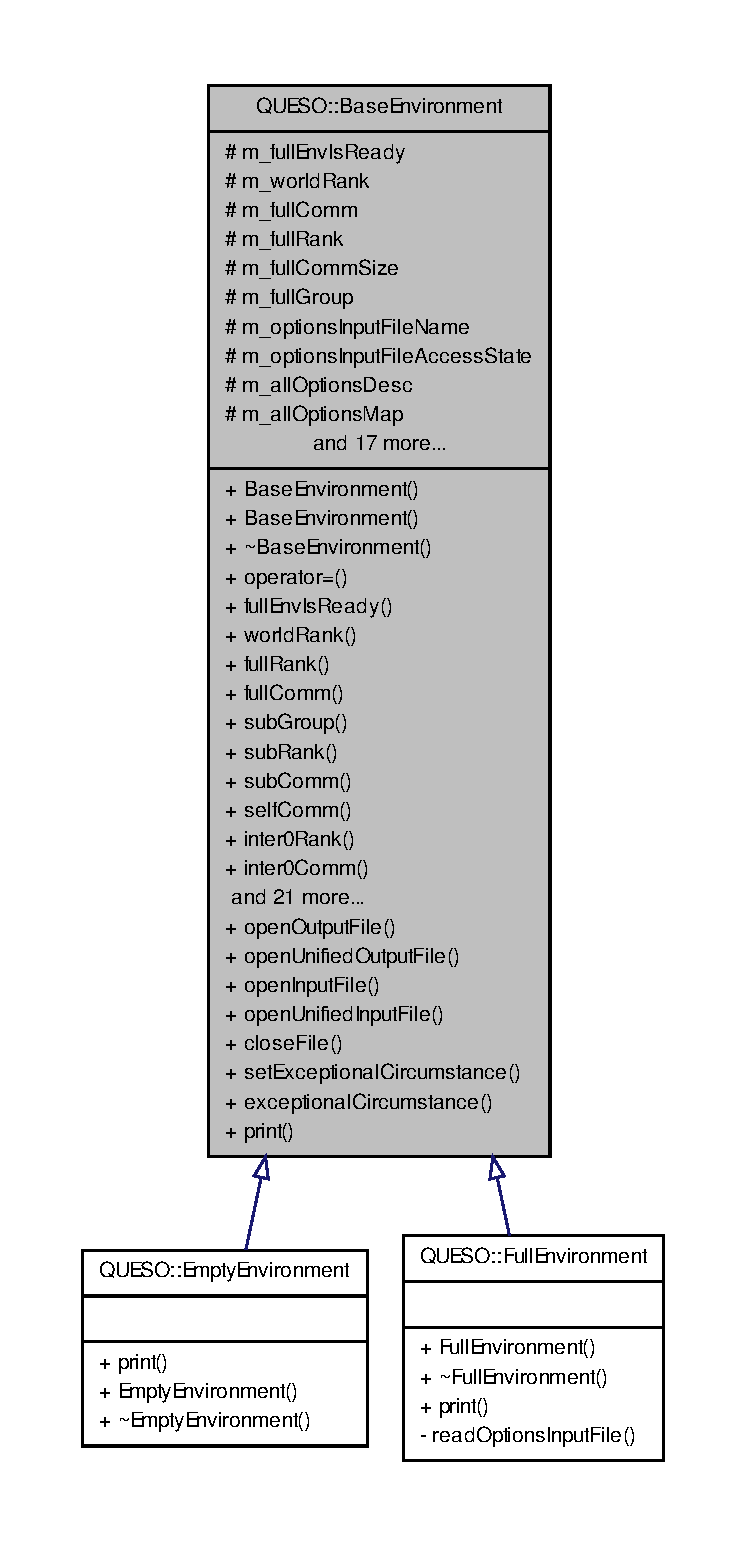
\includegraphics[scale=0.80,clip=true]{rawfigs/base_env_class.pdf}
\vspace*{-1.2cm}
\caption{The class diagram for the {Environment} class described in Section \ref{sec:environment_class}.}
\label{fig-env-class}
\end{figure}

\begin{figure}[!hp]
\centering
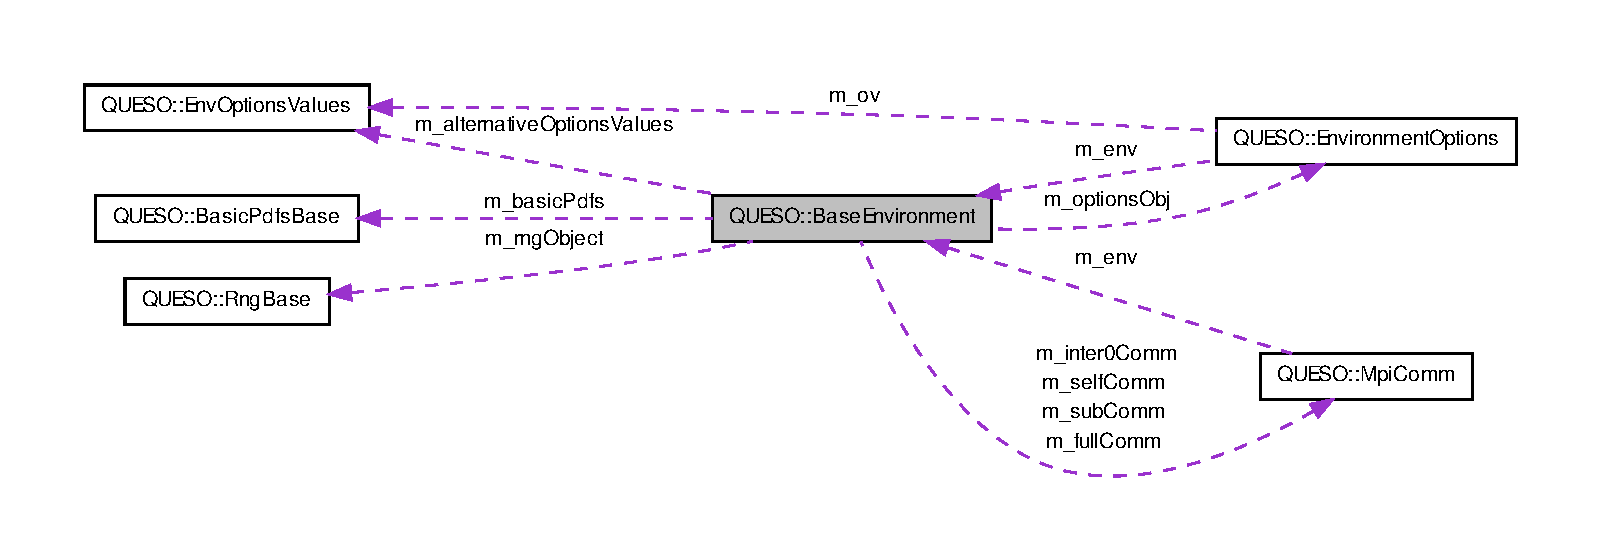
\includegraphics[scale=0.60,clip=true]{rawfigs/base_env_coll.pdf}
\vspace*{-1.cm}
\caption{Collaboration graph for the environment class described in Section \ref{sec:environment_class}.}
\label{fig-env-coll}
\end{figure}

\begin{figure}[htpb]
\centering
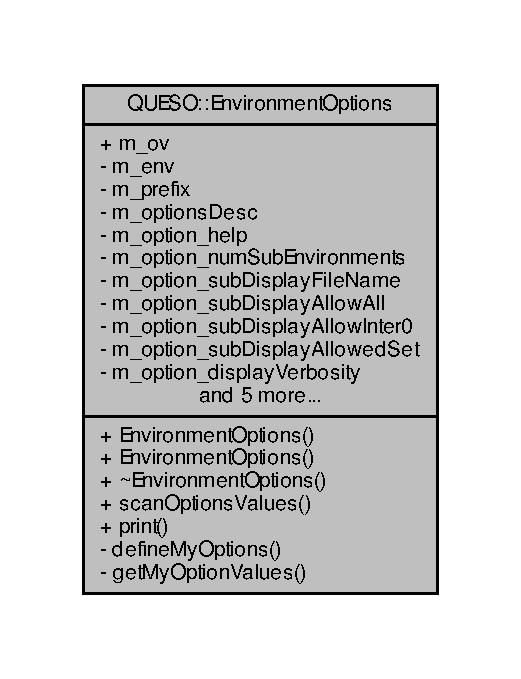
\includegraphics[scale=0.8,clip=true]{rawfigs/environment_options}
\vspace*{-1.2cm}
\caption{The environment options class with its attributes and methods.}
\label{fig-env-options-class}
\end{figure}

% \begin{figure}[!hp]
% \centering
% \includegraphics[scale=0.60,clip=true]{rawfigs/class_q_u_e_s_o_1_1_environment_options__coll__graph.pdf}
% \vspace*{-1.2cm}
% \caption{Collaboration graph for the environmentOption class.}% described in Section \ref{sec:environment_class}.}
% \label{fig-env-options-col}
% \end{figure}


% 
%\subsubsection{Input File Options}


\begin{table}[htpb]
\begin{center}
\caption{Input file options for a QUESO environment.}
\vspace{-8pt}
\label{tab-env-options}
\footnotesize
\begin{tabular}{l c  m{7cm}}
\toprule
Option name                      &  Default  value & Description \\
\midrule\midrule
\ttfamily \textlangle PREFIX\textrangle env\_help                &     & Produces help message for environment class            \\
%\midrule
\ttfamily\textlangle PREFIX\textrangle env\_numSubEnvironments   &  1  &  Number of subenvironments                \\ %UQ_ENV_NUM_SUB_ENVIRONMENTS_ODV
% \midrule
\ttfamily\textlangle PREFIX\textrangle env\_subDisplayFileName   & \ttfamily"." & Output filename for sub-screen writing     \\ %UQ_ENV_SUB_DISPLAY_FILE_NAME_ODV
% \midrule
\ttfamily\textlangle PREFIX\textrangle env\_subDisplayAllowAll   &  0  & Allows all subenvironments to write to output file \\ %UQ_ENV_SUB_DISPLAY_ALLOW_ALL_ODV
% \midrule
\ttfamily\textlangle PREFIX\textrangle env\_subDisplayAllowedSet & \ttfamily""  & Subenvironments that will write to output file \\ %UQ_ENV_SUB_DISPLAY_ALLOWED_SET_ODV
% \midrule
\ttfamily\textlangle PREFIX\textrangle env\_displayVerbosity     &  0  & Sets verbosity				         \\ %UQ_ENV_DISPLAY_VERBOSITY_ODV
% \midrule
\ttfamily\textlangle PREFIX\textrangle env\_syncVerbosity        &  0  & Sets syncronized verbosity             \\ %UQ_ENV_SYNC_VERBOSITY_ODV
% \midrule
\ttfamily\textlangle PREFIX\textrangle env\_seed                 &  0  & Set seed                             \\ %UQ_ENV_SEED_ODV
%
% TODO add the following options:
% (m_option_platformName.c_str(),         po::value<std::string >()->default_value(UQ_ENV_PLATFORM_NAME_ODV),           "platform name")""
% (m_option_identifyingString.c_str(),    po::value<std::string >()->default_value(UQ_ENV_IDENTIFYING_STRING_ODV),      "identifying string")""
% (m_option_checkingLevel.c_str(),        po::value<unsigned int>()->default_value(UQ_ENV_CHECKING_LEVEL_ODV),          "set checking level")  0          
\bottomrule
\end{tabular}
\end{center}
\end{table}

  

%\clearpage
\subsection{Vector}\label{sec:vector_class}


The Vector class handles all the vector operations carried out in QUESO, and currently has two derived classes: \verb+GslVector+ and \verb+TeuchosVector+. \verb+GslVector+ is based on the GSL vector structure; whereas \verb+TeuchosVector+ is based on Trilinos Teuchos vector structure~\cite{Trilinos}, and therefore, it is only available if QUESO was compiled with Trilinos.  

A class diagram for \verb+Vector+ class is presented in Figure \ref{fig-vector-class}.%; the reader may notice that the diagram also presents an extra class, \verb+PetscVector+, in order to show QUESO flexibility to the inclusion of other classes -- this class has yet to be implemented.


\begin{figure}[!htpb]
\centering
\vspace*{-.5cm}
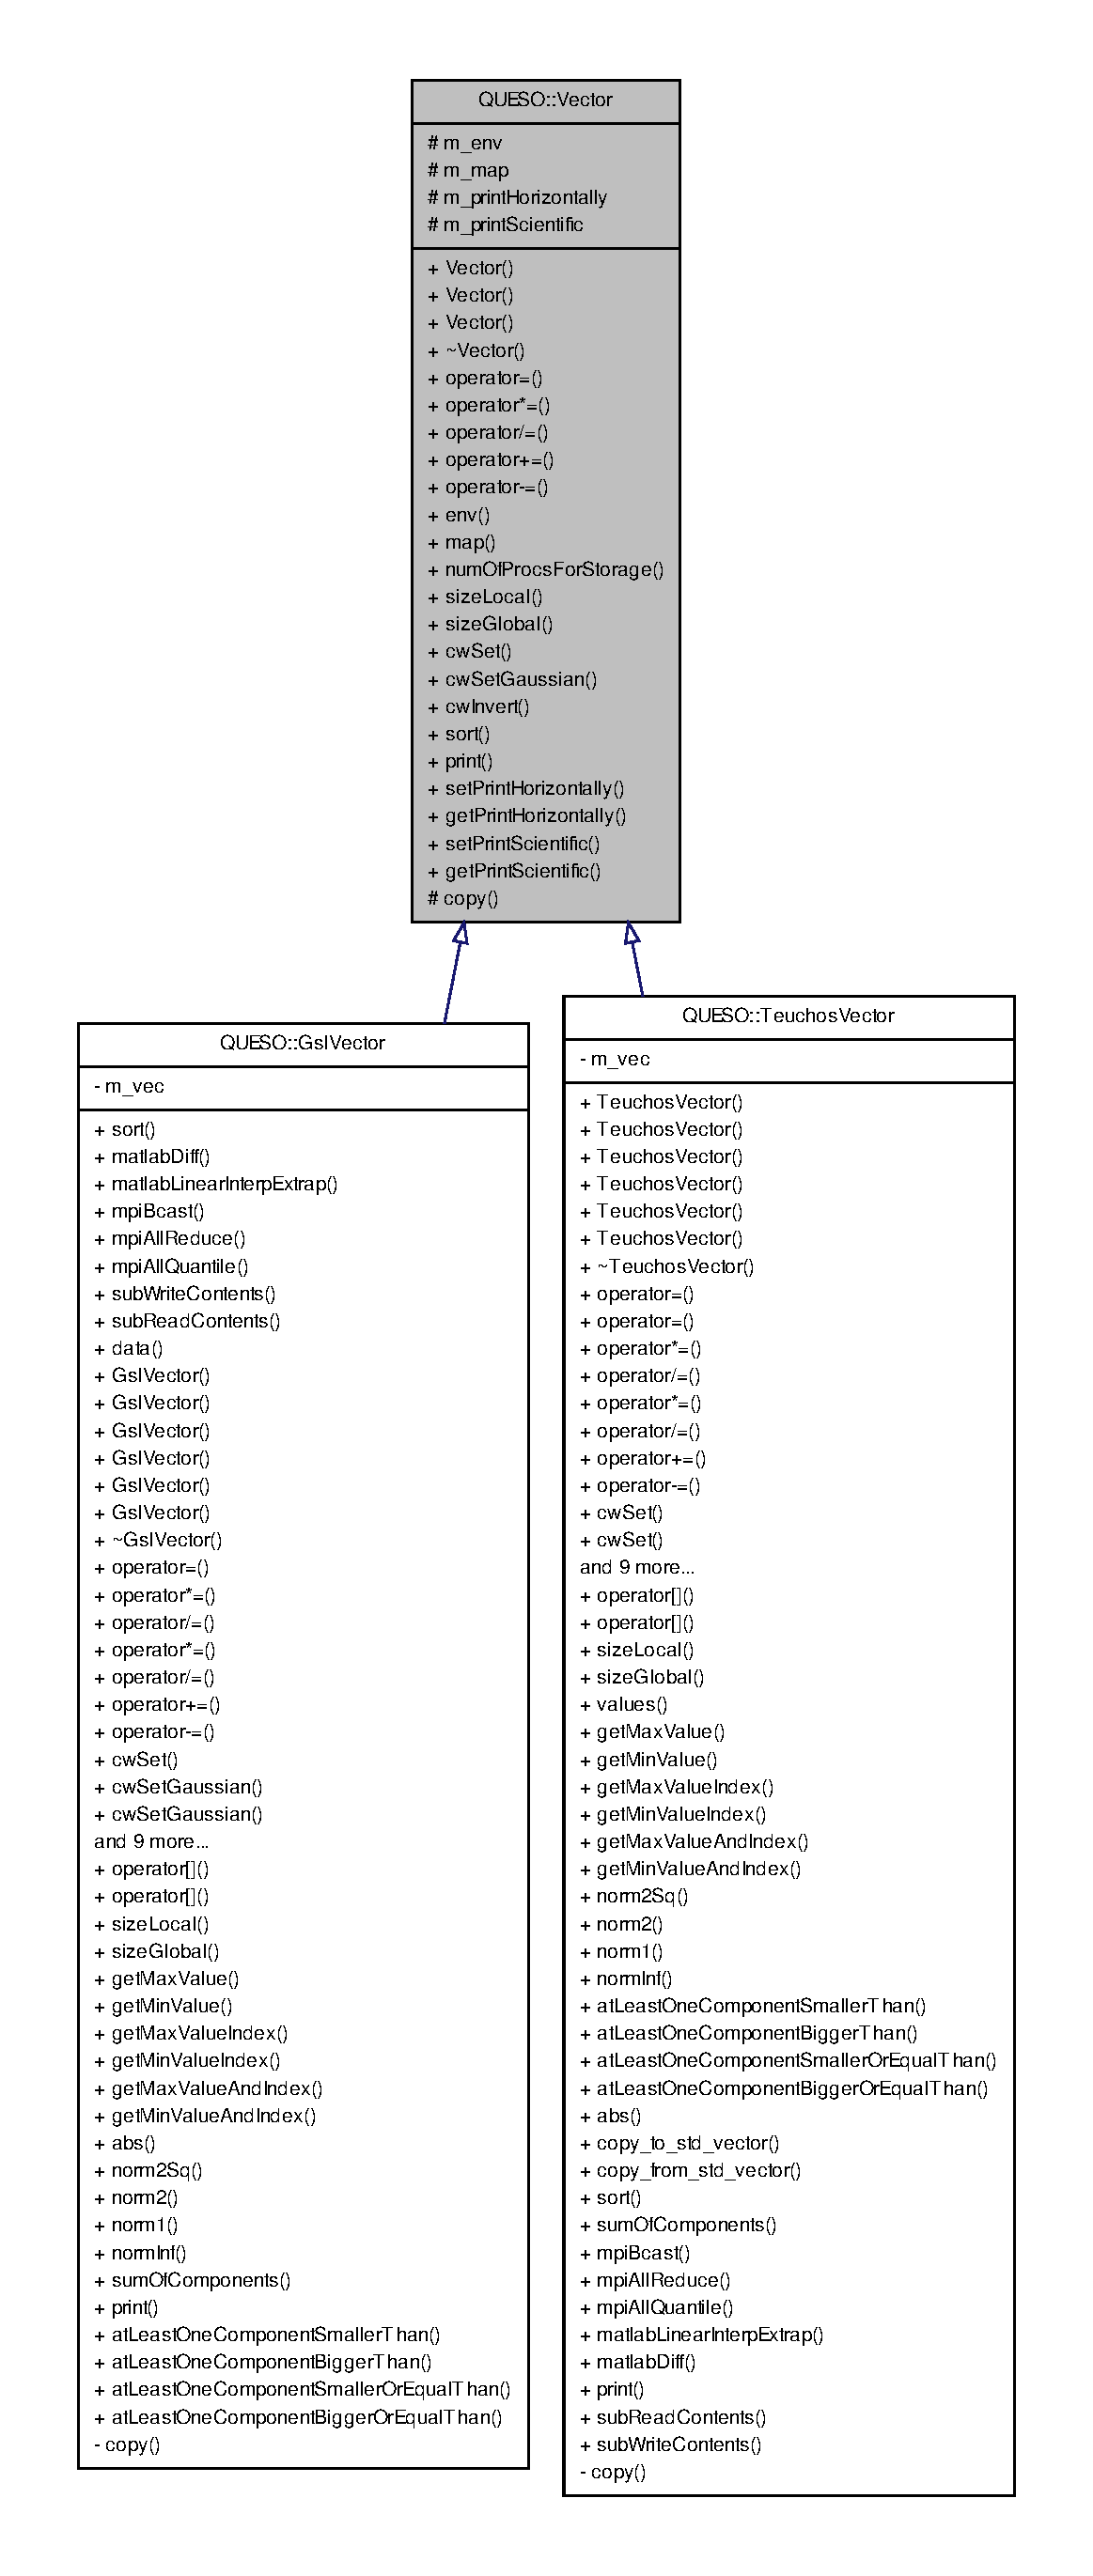
\includegraphics[scale=0.50,clip=true]{rawfigs/vector}
\vspace*{-.8cm}
\caption{ The class diagram for the vector class described in Section \ref{sec:vector_class}.}
\label{fig-vector-class}
\end{figure}



\subsection{Matrix}\label{sec:matrix_class}

% The Matrix class handles all the matrix operations carried out in QUESO, and its class diagram is presented in Figure \ref{fig-matrix-class}. Analogously to the Vector class case,
% Matrix class has two derived classes: \verb+GslMatrix+ and \verb+TeuchosMatrix+. \verb+GslMatrix+ is based on the GSL matrix structure; whereas \verb+TeuchosMatrix+ is based on Trilinos Epetra matrix structure.


The Matrix class handles all the matrix operations carried out in QUESO.  Analogously to the vector class case described in the previous section,
matrix class currently has two derived classes: \verb+GslMatrix+ and \verb+TeuchosMatrix+. \verb+GslMatrix+ is based on the GSL matrix structure; whereas \verb+TeuchosMatrix+ is based on Trilinos Epetra matrix structure.

A class diagram for \verb+Matrix+  is presented in Figure \ref{fig-matrix-class}; it displays its protected attributes together with its member functions. Again, the diagram displays in some detail the inherited classes \verb+GslMatrix+ and \verb+TeuchosMatrix+.


\begin{figure}[!hp]
\centering
\vspace*{-.8cm}
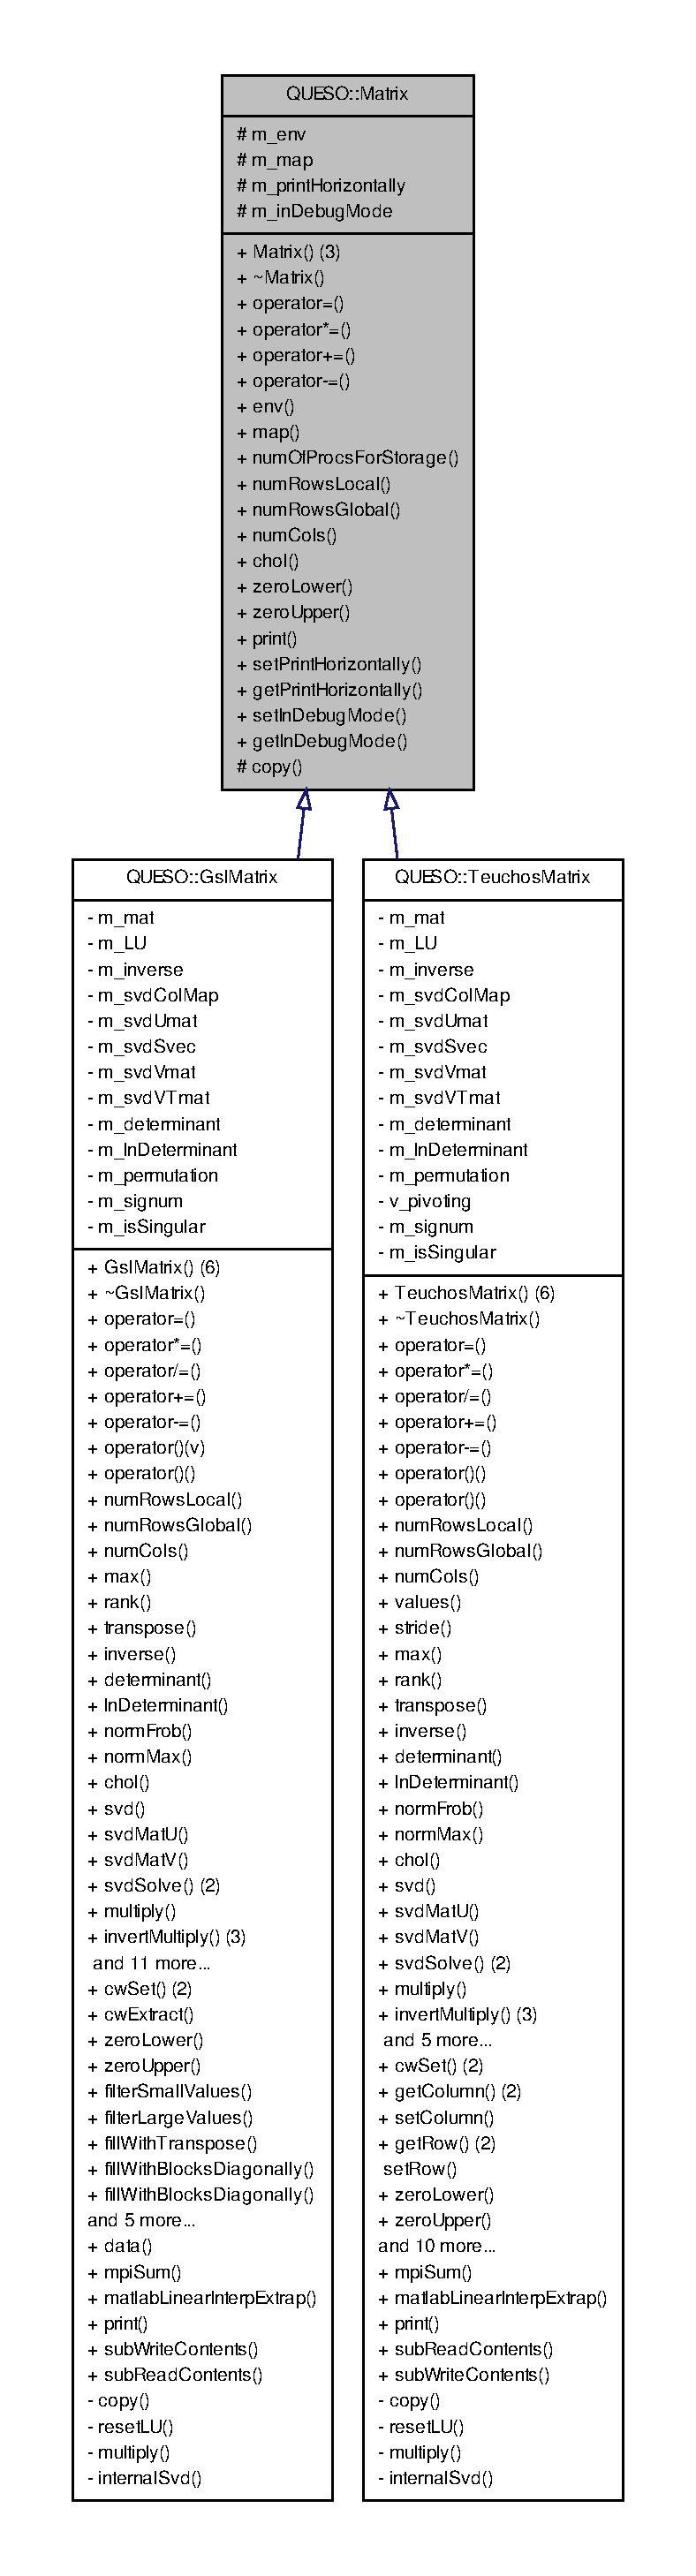
\includegraphics[scale=0.50,clip=true]{rawfigs/matrix}
\vspace*{-.8cm}
\caption{The class diagram for the matrix class.}% described in Section \ref{sec:matrix_class}.}
\label{fig-matrix-class}
\end{figure}


%\clearpage
\section{Templated Basic Classes}
The classes in this group are: vector sets, subsets and spaces (Section \ref{sec:vector-set-space}), scalar and vector function classes (Section \ref{sec:scalar-vector-function}), and scalar and vector sequences (Section \ref{sec:scalar-vector-sequence}).

These classes constitute the core entities necessary for the formal
mathematical definition and description of other entities, such as
random variables, Bayesian solutions of inverse problems, sampling algorithms and chains.

%\clearpage


\subsection{Vector Set, Subset  and Vector Space Classes}\label{sec:vector-set-space}
%
The vector set class is fundamental for the proper handling of many mathematical entities.
Indeed, the definition of a scalar function such as $\pi:\mathbf{B}\subset\mathbb{R}^n\rightarrow\mathbb{R}$ requires the
specification of the domain $\mathbf{B}$, which is a {\it subset} of the {\it vector space} $\mathbb{R}^n$, which is itself a {\it set}. Additionally, 
 SIPs need a likelihood routine $\pi_{\text{like}}:\mathbb{R}^n\rightarrow\mathbb{R}_+$,
and SFPs need a QoI routine $\mathbf{q}:\mathbb{R}^n\rightarrow\mathbb{R}^m$; the \textit{sets} $\mathbb{R}^n$, $\mathbb{R}^m$, etc., are {\it vector spaces}.


The relationship amongst QUESO classes for handling sets, namely \verb+VectorSet+; subsets, namely \verb+VectorSubset+;  and vector spaces, namely \verb+VectorSpace+ is sketched in Figure \ref{fig-vector-space-subset-classes}.
%
An attribute of the {\it subset} class is the {\it vector space} which it belongs to, and in fact a reference to a vector space is required by the constructor of the subset class. An example of this case is the definition of a scalar function such as $\pi:\mathbf{B}\subset\mathbb{R}^n\rightarrow\mathbb{R}$ above. %, which requires the specification of the domain $\mathbf{B}$, which is a {\it subset} of the {\it vector space} $\mathbb{R}^n$, which is itself a {\it set}.

The power of an object-oriented design is clearly featured here.
The intersection subset derived class \verb+IntersectionSubset+ is useful for handling a posterior PDF  on Equation~\eqref{eq-Bayes-solution},
since its domain is the intersection of the domain of the prior PDF with the domain of the likelihood function.

\begin{figure}[htpb]
% \centering
\hspace{-1cm}
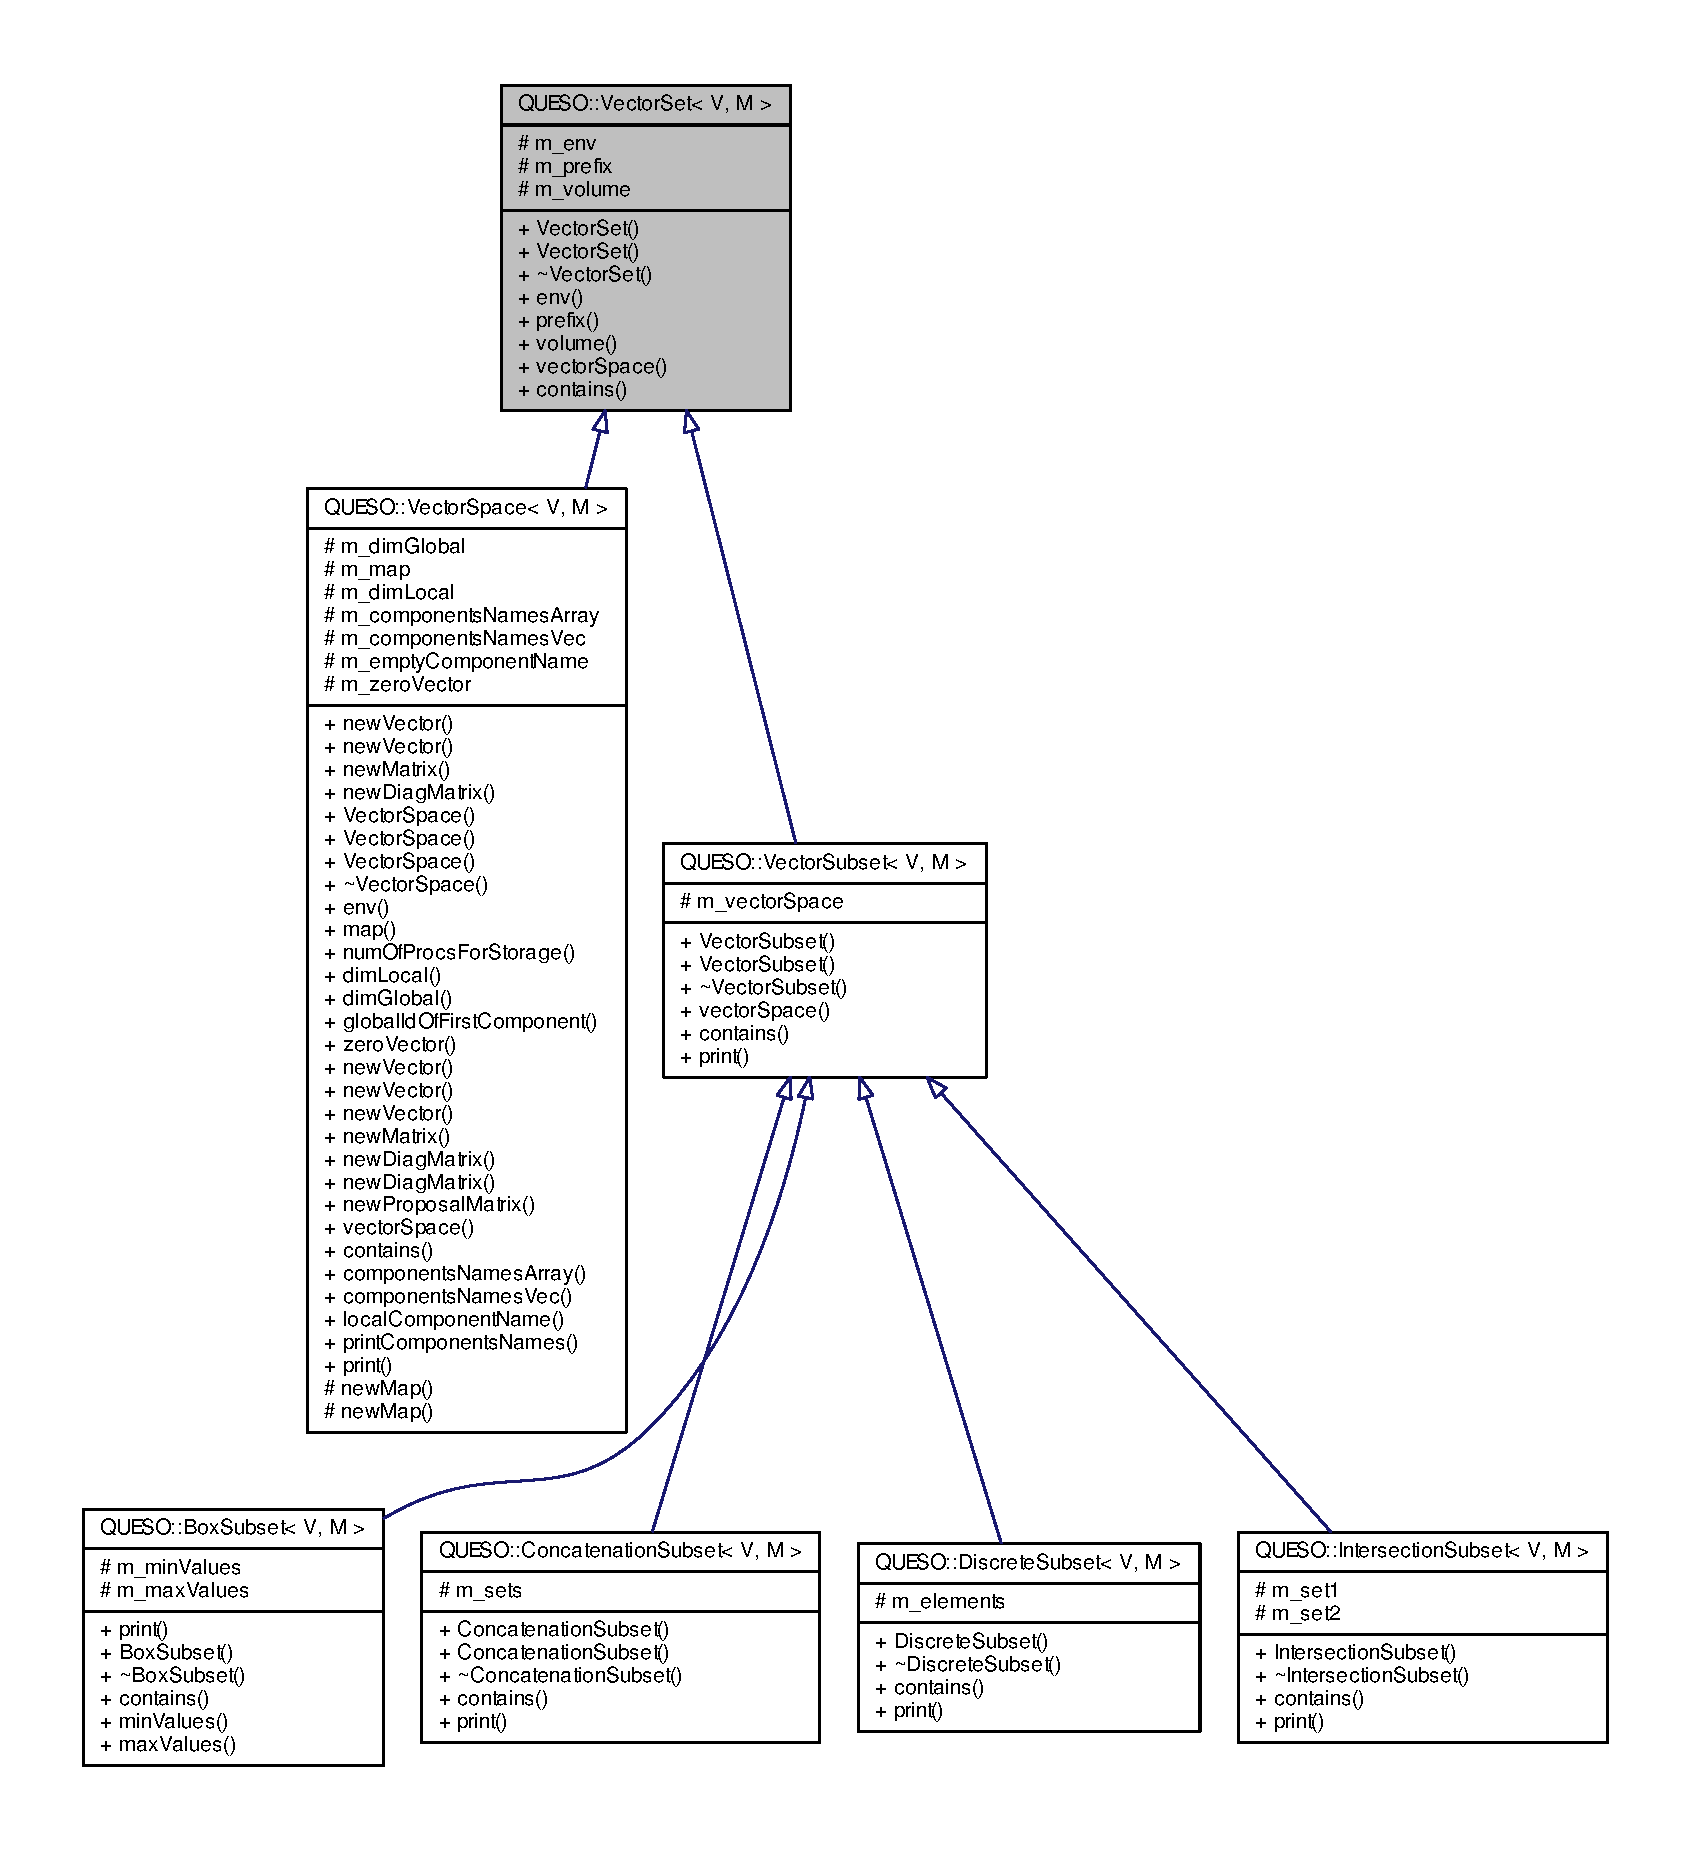
\includegraphics[scale=0.65,clip=true]{rawfigs/vector_set}
\vspace*{-1.5cm}
\caption{The class diagram for vector set, vector subset and vector space classes, described in Section \ref{sec:vector-set-space}.}
\label{fig-vector-space-subset-classes}
\end{figure}

% 
% \begin{figure}[htpb]
% % \centering
% \hspace{-1cm}
% \includegraphics[scale=0.65,clip=true]{rawfigs/class_q_u_e_s_o_1_1_vector_set__coll__graph}
% \vspace*{-1.5cm}
% \caption{Collaboration graph of VectorSet class.}
% \label{fig-vector-space-subset-classes}
% \end{figure}



%\clearpage
\subsection{Scalar Function and Vector Function Classes}\label{sec:scalar-vector-function}

Joint PDF, marginal PDF, and CDF are all examples of scalar functions present in statistical problems. 
QUESO currently supports basic PDFs such as uniform and Gaussian and also more complex PDFs, such as the ones coming from a Bayesian analysis. They are implemented in the classes \verb+UniformJointPdf+, \verb+GaussianJointPdf+, and \verb+BayesianJointPdf+, respectively. The posterior PDF may be represented within QUESO by \verb+GenericJointPdf+.
See Diagram~\ref{fig-scalar-function-class} for the scalar function class.

The handling of vector functions within QUESO is also quite straightforward. Indeed, the definition of a vector function $\mathbf{q}:\mathbf{B}\subset\mathbb{R}^n\rightarrow\mathbb{R}^m$ requires only the extra specification of the image vector space $\mathbb{R}^m$. The classes representing the vector function class \verb+GenericVectorFunction+ and \verb+ConstantVectorFunction+ are derived  from \verb+BaseVectorFunction+ and are presented in Diagram \ref{fig-vector-function-class} 
\begin{figure}[htpb]
% \centering
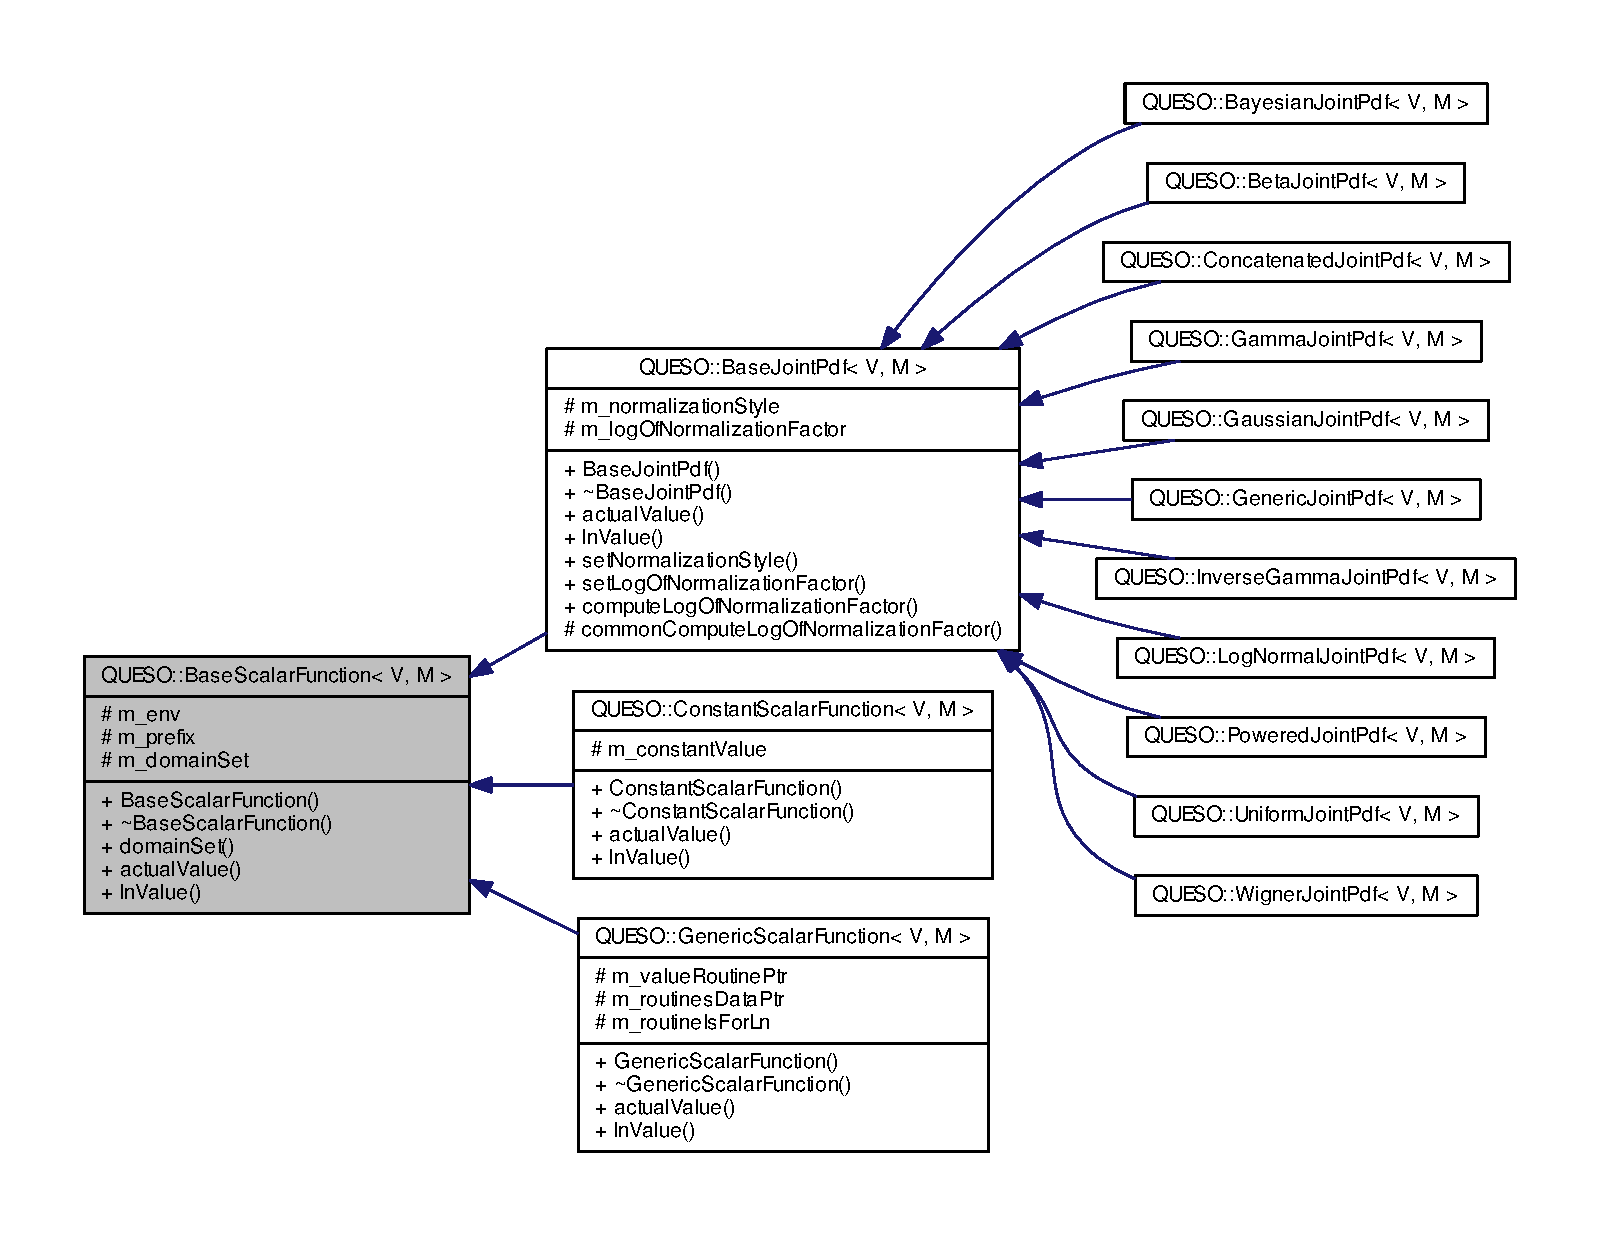
\includegraphics[scale=0.65,clip=true]{rawfigs/base_scalar_function}
\vspace*{-1.5cm}
\caption{The class diagram for the scalar function class.}
\label{fig-scalar-function-class}
\end{figure}

\begin{figure}[htpb]
\centering
\hspace{-40pt}
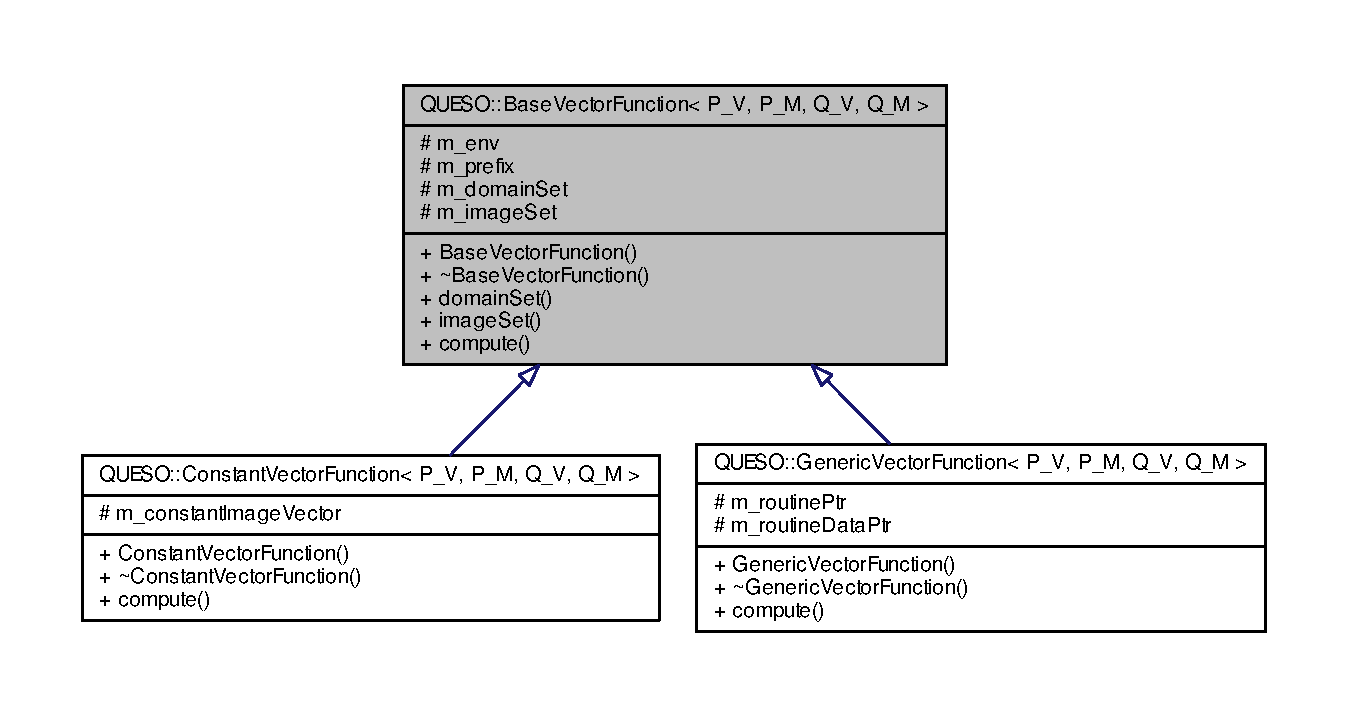
\includegraphics[scale=0.65,clip=true]{rawfigs/base_vector_function.pdf}
\vspace{-1.2cm}
\caption{The class diagram for the vector function class described in Section \ref{sec:scalar-vector-function}.} % new fig: added uqConstantVectorFunctionClass on 12/17/12.
\label{fig-vector-function-class}
\end{figure}

%\clearpage

\subsection{Scalar Sequence and Vector Sequence Classes}\label{sec:scalar-vector-sequence}
%
The scalar sequence class contemplates {\it scalar} samples generated by an algorithm, as well as operations that can
be done over them, e.g., calculation of means, variances, and convergence indices.
%% such as Geweke and Brooks-Gelman.
Similarly, the vector sequence class contemplates {\it vector} samples and operations such as means, correlation matrices and covariance matrices.

Figures \ref{fig-scalar-sequence-class} and \ref{fig-vector-sequence-class} display the class diagram for the scalar sequence  and vector sequence classes, respectively.

\begin{figure}[htpb]
\centering
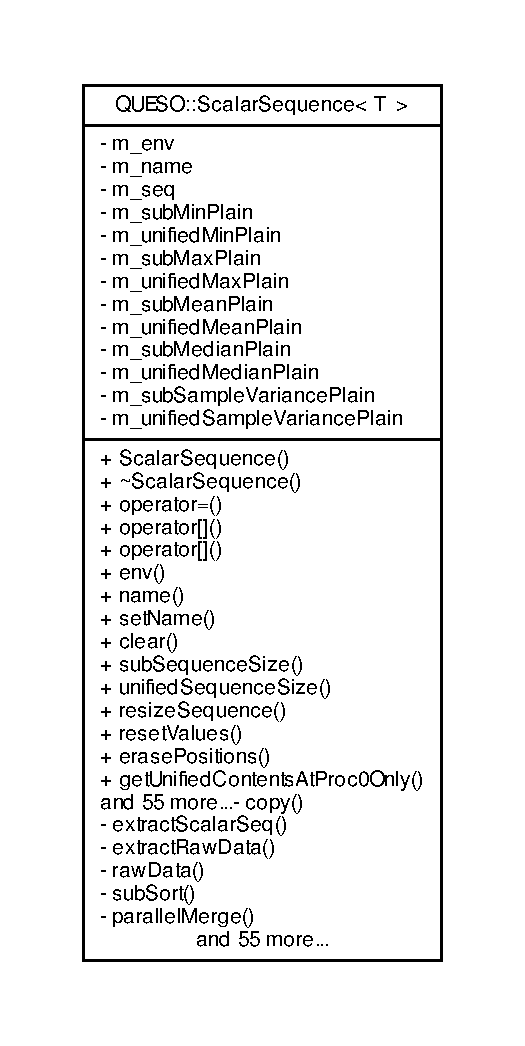
\includegraphics[scale=0.65,clip=true]{rawfigs/scalar_sequence}
\vspace{-1.cm}
\caption{The class diagram for the scalar sequence class.}
\label{fig-scalar-sequence-class}
\end{figure}

\begin{figure}[htpb]
\centering
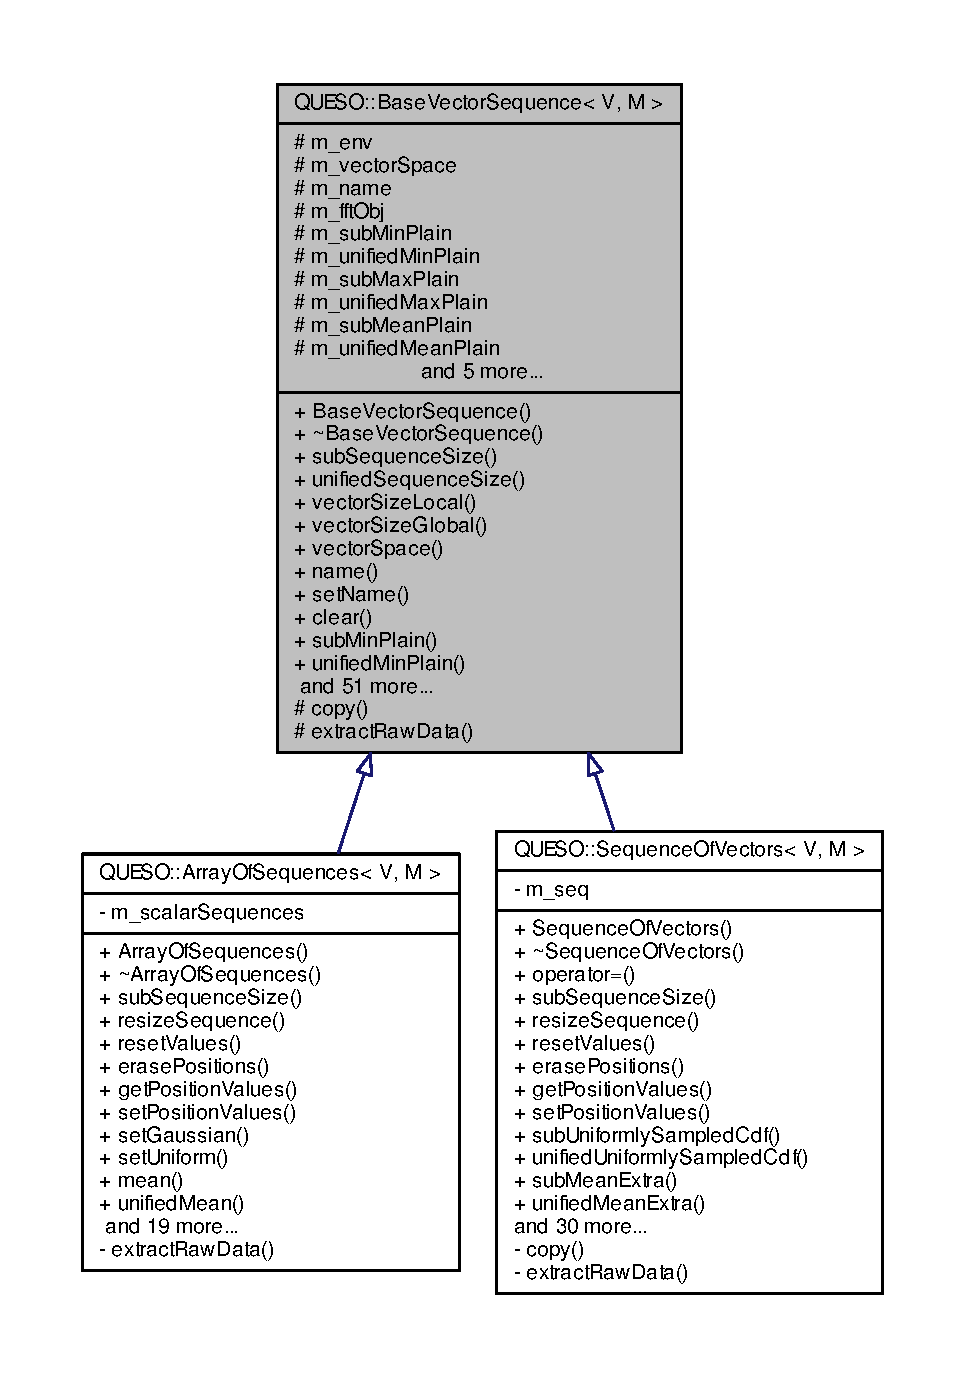
\includegraphics[scale=0.65,clip=true]{rawfigs/vector_sequence}
\vspace{-1.cm}
\caption{The class diagram for the vector sequence class.}
\label{fig-vector-sequence-class}
\end{figure}



%\clearpage
\section{Templated Statistical Classes}

The classes in this group are: vector realizer, vector random variable, statistical inverse problem (and options), Metropolis-Hastings solver (and options), statistical forward problem (and options), Monte Carlo solver (and options), and Sequence statistical options.

For QUESO, a SIP has two input entities, a prior RV and
a likelihood routine, and one output entity, the posterior RV, as shown in Chapter \ref{ch-introduction}, Figure~\ref{fig-sip-queso}.
%
Similarly, a SFP has two input entities, a input RV and
a QoI routine, and one output entity, the output RV, as shown in Figure \ref{fig-sfp-queso}.


\subsection{Vector Realizer Class}\label{sec:vector-realizer-class}
%
A {\it realizer} is an object that, simply put, contains a \verb+realization()+ operation that returns a sample of a vector RV.
QUESO currently supports several realizers: 
\begin{itemize}
 \item uniform, implemented in \verb+UniformVectorRealizer+,                \vspace{-8pt}
\item Gaussian, implemented in \verb+GaussianVectorRealizer+,               \vspace{-8pt}
\item Log Normal, implemented in \verb+LogNormalVectorRealizer+,            \vspace{-8pt}
\item Gamma,  implemented in \verb+GammaVectorRealizer+,                    \vspace{-8pt}
\item Inverse Gamma, implemented in \verb+InverseGammaVectorRealizer+, and  \vspace{-8pt}
\item Beta, , implemented in \verb+BetaVectorRealizer+,                     \vspace{-8pt}
\end{itemize}
which are all derived from the base class \verb+BaseVectorRealizer+. 
 
QUESO conveniently provides the class \verb+ConcatenatedVectorRealizer+, which allows two distinct realizers to be concatenated.
It also contains a {\it sequence realizer} class for storing samples of a MH algorithm. 




\subsection{Vector Random Variable Class}
%
Vector RVs are expected to have two basic functionalities:
compute the value of its PDF at a point, and generate realizations following such PDF.
The joint PDF (\verb+BaseJointPdf+ and derived classes, see Section \ref{sec:scalar-vector-function}) and vector realizer  (\verb+BaseVectorRealizer+ and derived classes, see Section \ref{sec:vector-realizer-class}) classes allow a straightforward definition and manipulation of vector RVs. Similarly to the vector realizer class above, QUESO also allows users to form new RVs through the concatenation of existing RVs (class \verb+ConcatenatedVectorRV+).

QUESO currently supports a few vector RVs such as uniform, Gaussian, Gamma and Beta, as depicted in Diagram \ref{fig-vector-rv-class}.
A derived class called {\it generic vector RV} allows QUESO to store the solution of an statistical IP:
a {\it Bayesian joint PDF} becomes the PDF of the posterior RV, while a {\it sequence vector realizer} becomes the realizer of the same posterior RV.



\begin{figure}[htpb]
\centering
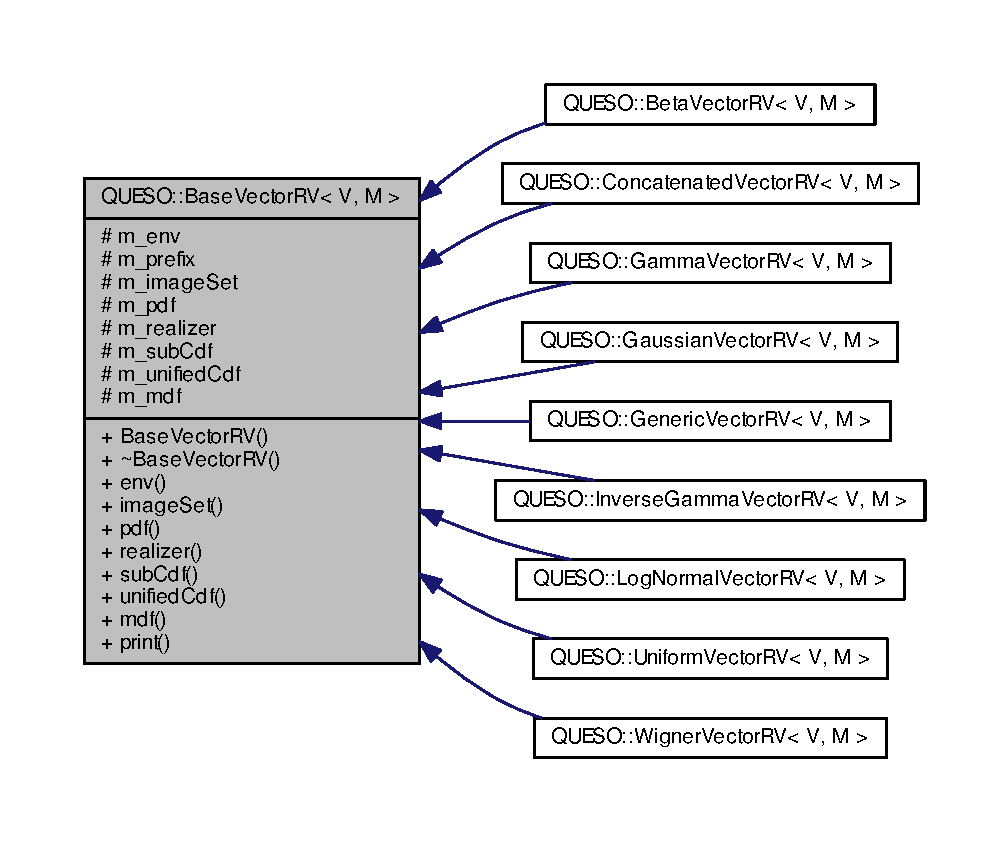
\includegraphics[scale=0.7,clip=true]{rawfigs/vector_rv}
\vspace{-1.cm}
\caption{The class diagram for the vector random variable class.}
\label{fig-vector-rv-class}
\end{figure}



%\clearpage
\subsection{Statistical Inverse Problem (and Options)}
Similarly to its mathematical concepts, a SIP in QUESO also expects two input entities, a prior RV and a likelihood routine, and one output entity, the posterior RV.
The SIP is represented in QUESO through the templated class \verb+StatisticalInverseProblem<P_V,P_M>+, which is illustrated in Figure \ref{fig-sip-class}.
One important characteristic of the QUESO design is that it  separates `what the problem is' from `how the problem is solved'.
The prior and the posterior RV are instances of the \verb+BaseVectorRv<V,M>+ class, while
the likelihood function is an instance of the \verb+BaseScalarFunction<V,M>+ class.

The solution of a SIP is computed by calling either \verb+solveWithBayesMetropolisHastings()+ or \verb+solveWithBayesMLSampling()+, which are member functions of the class\linebreak\verb+StatisticalInverseProblem<P_V,P_M>+ class.
Upon return from a solution operation, the posterior RV is available through the \verb+postRv()+ member function.
More details are provided about \verb+solveWithBayesMetropolisHastings()+ and \verb+solveWithBayesMLSampling()+ in Sections \ref{sec:MH} and \ref{sec:ML}, respectively.

Figure \ref{fig-sip-options-class} displays the  \verb+StatisticalInverseProblemOptions+ class, i.e. that class that handles a variety of options for solving the SIP. Such options may be provided to QUESO by the user's input file; and they are listed in Table \ref{tab-sip-options}.


\begin{figure}[htpb]
\centering
\subfloat[StatisticalInverseProblem]{
 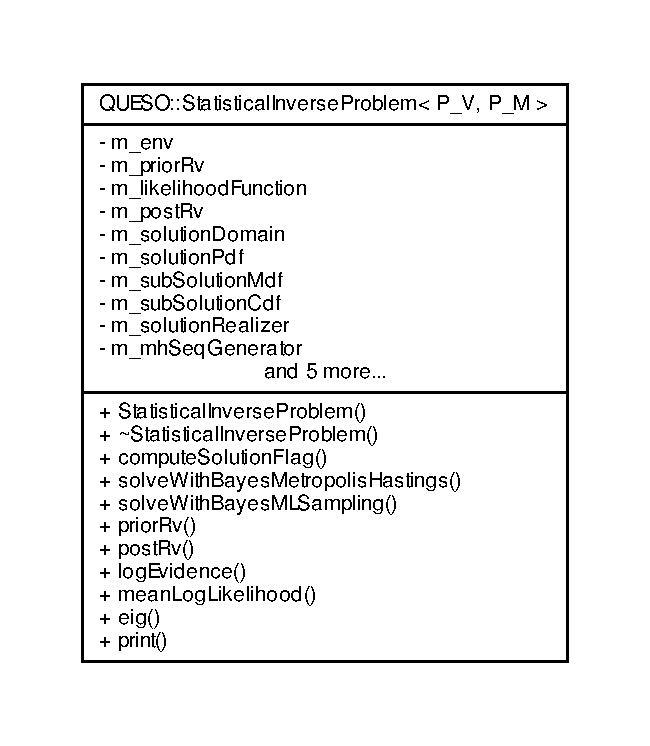
\includegraphics[trim={0 1.3cm 0 0},clip,scale=0.8]{rawfigs/statistical_inverse_problem}\label{fig-sip-class}}
\subfloat[StatisticalInverseProblemOptions]{
 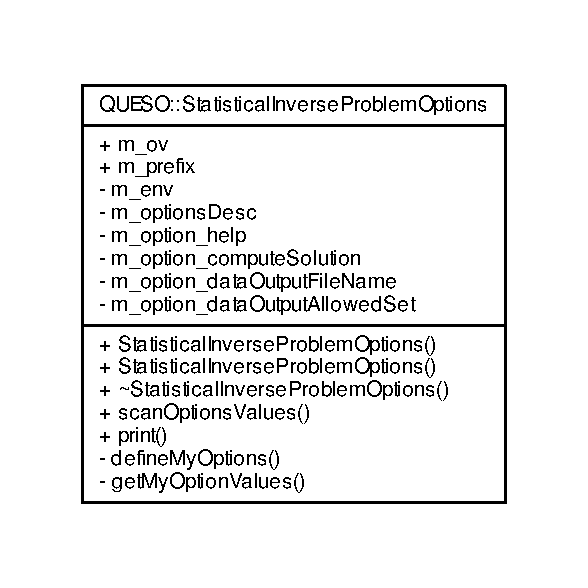
\includegraphics[trim={0 1.3cm 0 0},clip,scale=0.8]{rawfigs/statistical_inverse_problem_options}\label{fig-sip-options-class}}
\vspace{-.2cm}
\caption{The statistical inverse problem class, which implements the representation in Figure~\ref{fig-sip-queso}, and statistical inverse problem options class.}
\end{figure}



\begin{table}[htpb]
\begin{center}
\caption{Input file options for a QUESO statistical inverse problem.}
\vspace{-8pt}
\label{tab-sip-options}
\ttfamily\footnotesize
\begin{tabular}{l c  m{7cm}}
\toprule
\rmfamily Option name                    & \rmfamily Default  Value & \rmfamily Description \\
\midrule\midrule
\textlangle PREFIX\textrangle ip\_help                 &     &  \rmfamily Produces help message for statistical inverse problem   \\
% \midrule
\textlangle PREFIX\textrangle ip\_computeSolution      &  1  &  \rmfamily Computes solution process \\% UQ_SIP_COMPUTE_SOLUTION_ODV
% \midrule
\textlangle PREFIX\textrangle ip\_dataOutputFileName   & "." &  \rmfamily Name of data output file \\%UQ_SIP_DATA_OUTPUT_FILE_NAME_ODV
% \midrule
\textlangle PREFIX\textrangle ip\_dataOutputAllowedSet & ""  &  \rmfamily Subenvironments that will write to data output file  \\%UQ_SIP_DATA_OUTPUT_ALLOWED_SET_ODV
\bottomrule
\end{tabular}
\end{center}
\end{table}


%\clearpage
\subsection{Metropolis-Hastings Solver (and Options)}\label{sec:MH}


The templated class that represents a Metropolis-Hastings generator of samples in QUESO is \verb+MetropolisHastingsSG<P_V,P_M>+, where SG stands for 'Sequence Generator'. This class implements the DRAM algorithm of Haario, Laine, Mira and Saksman~\cite{HaLaMiSa06} together with an operation named \verb+generateSequence()+ 
based on the core routine at the MCMC toolbox for MATLAB~\cite{Mcmctool}. %In fact,, the reader may notice that the example available in the QUESO build tree directory \verb+examples/statisticalInverseProblem+ is closely related to the `normal example' in the toolbox.


The Metropolis-Hastings sequence generator class is depicted in Figure \ref{fig-metropolis-hastings-solver-class}; the Metropolis-Hastings sequence generator options class is depicted in Figure \ref{fig-metropolis-hastings-options-class}. A collaboration graph for the Metropolis-Hastings class is presented in Figure \ref{fig-metropolis-hastings-coll}; and the options are presented in Table \ref{tab-metropolis-hastings-options}.

% \begin{figure}[htpb]
% \centering
% \subfloat[MetropolisHastingsSG]{\label{fig-metropolis-hastings-solver-class}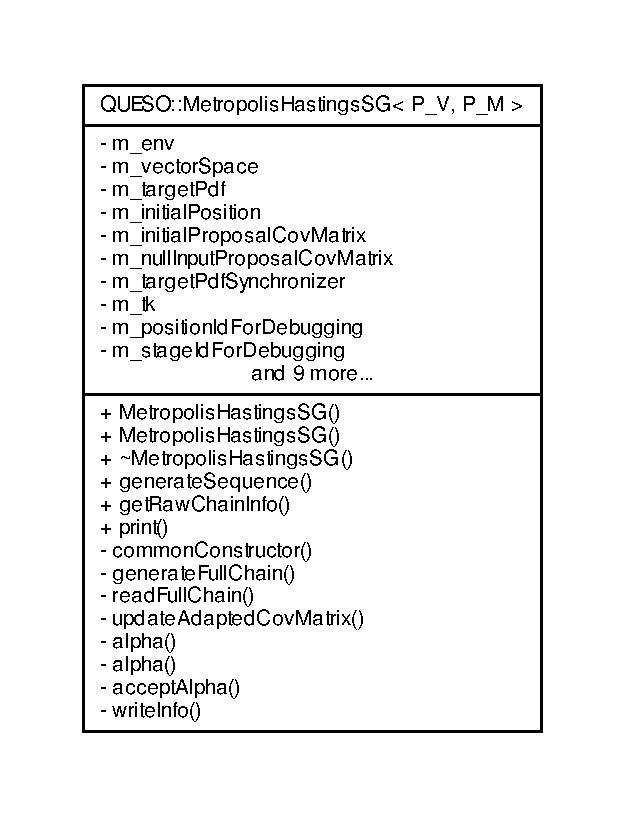
\includegraphics[trim={0 1.3cm 0 0},clip, scale=0.65]{rawfigs/metropolis_hastings}}
% \subfloat[MetropolisHastingsSGOptions]{\label{fig-metropolis-hastings-options-class}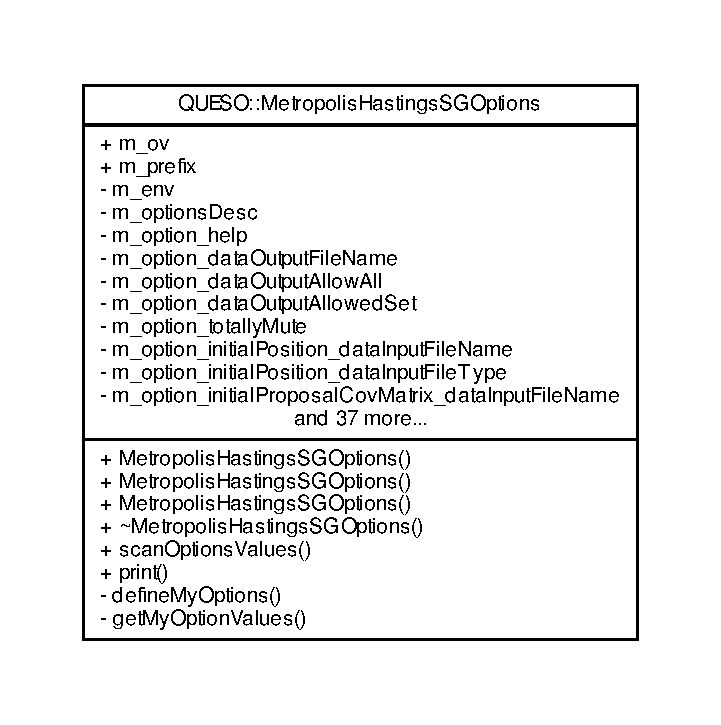
\includegraphics[trim={0 1.3cm 0 0},clip, scale=0.65]{rawfigs/metropolis_hastings_options}}
% \vspace{-.2cm}
% \caption{The Metropolis-Hastings sequence generator class and the Metropolis-Hastings sequence generator options class.}
% \end{figure}


\begin{figure}[htpb]
\centering
\subfloat[MetropolisHastingsSG]{\label{fig-metropolis-hastings-solver-class}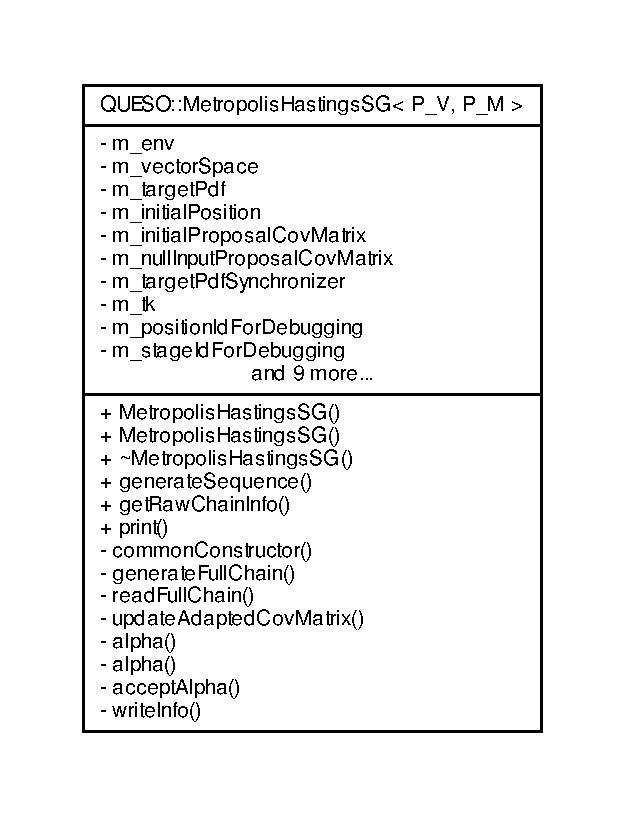
\includegraphics[trim={0 1.3cm 0 0},clip, scale=0.65]{rawfigs/metropolis_hastings}}
\subfloat[MetropolisHastingsSGOptions]{\label{fig-metropolis-hastings-options-class}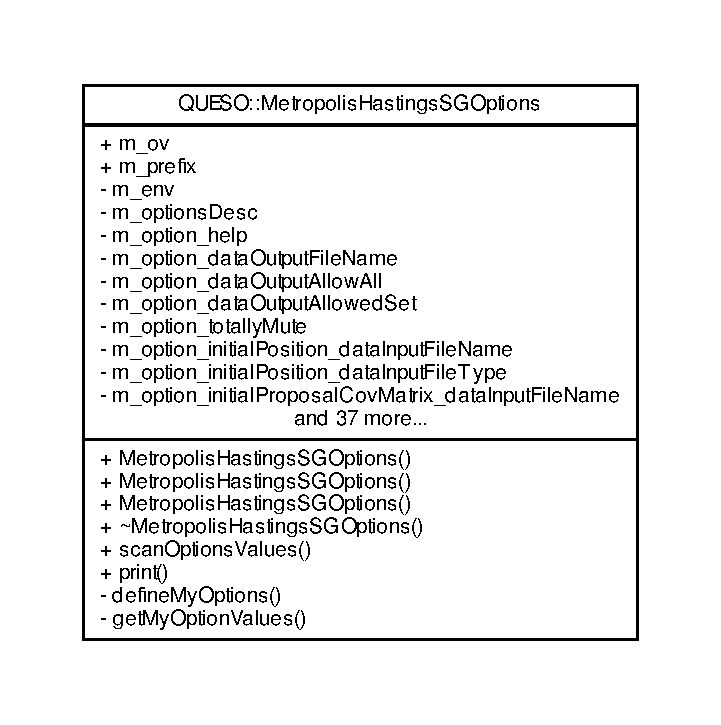
\includegraphics[trim={0 1.3cm 0 0},clip, scale=0.65]{rawfigs/metropolis_hastings_options}}
\vspace{-.2cm}
\caption{The Metropolis-Hastings sequence generator class and the Metropolis-Hastings sequence generator options class.}
\end{figure}

% Use the trim option, which takes four space separated values: 
%  trim={<left> <lower> <right> <upper>}
% 
% \begin{figure}[htpb]
% \centering
% 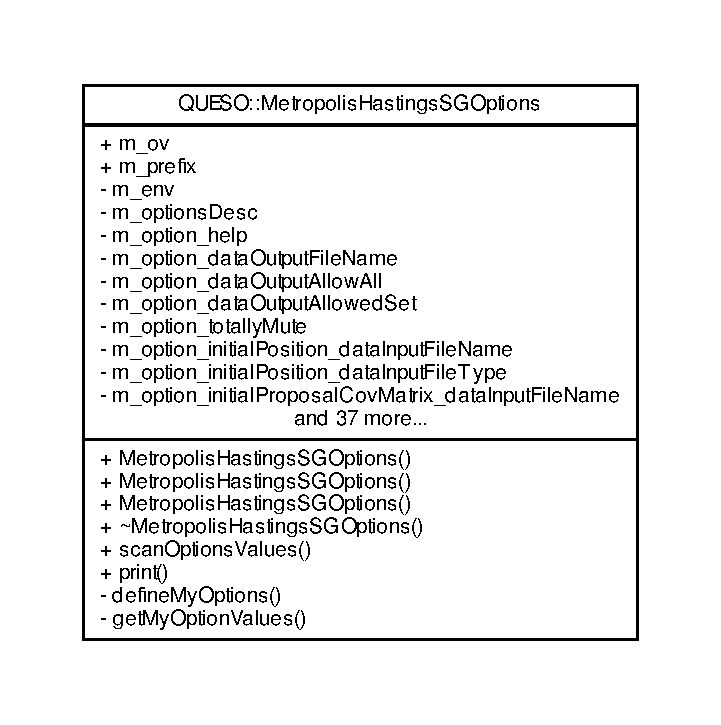
\includegraphics[scale=0.65,clip=true]{rawfigs/metropolis_hastings_options}
% \vspace{-1.2cm}
% \caption{The Metropolis-Hastings sequence generator options class.}
% \label{fig-metropolis-hastings-options-class}
% \end{figure}


\begin{figure}[p]
\centering
% 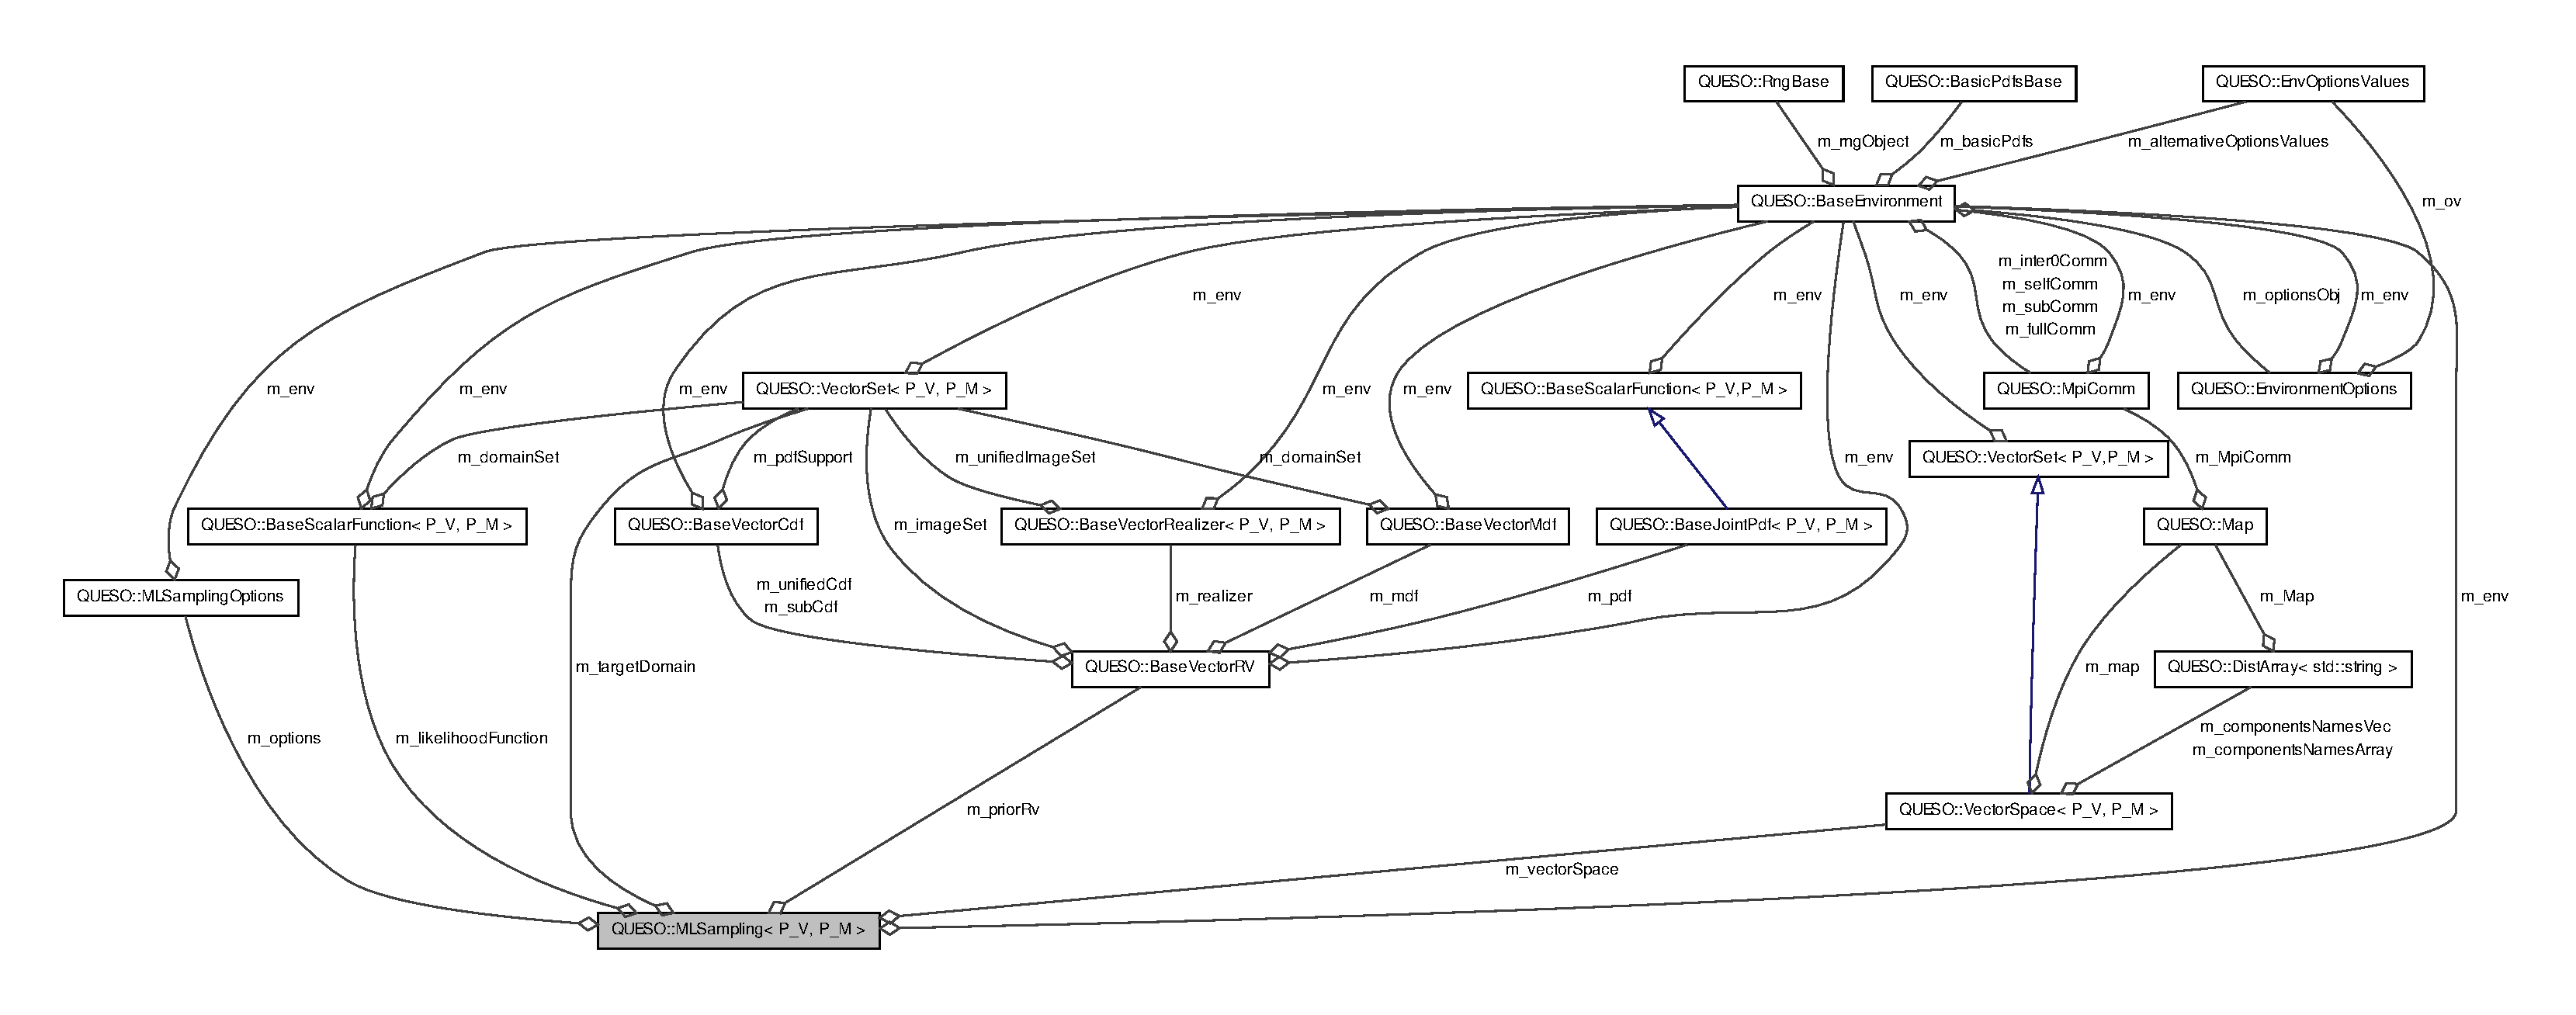
\includegraphics[width=1.3\textwidth, height=.7\textheight,clip=true,angle=90]{rawfigs/ml_coll}
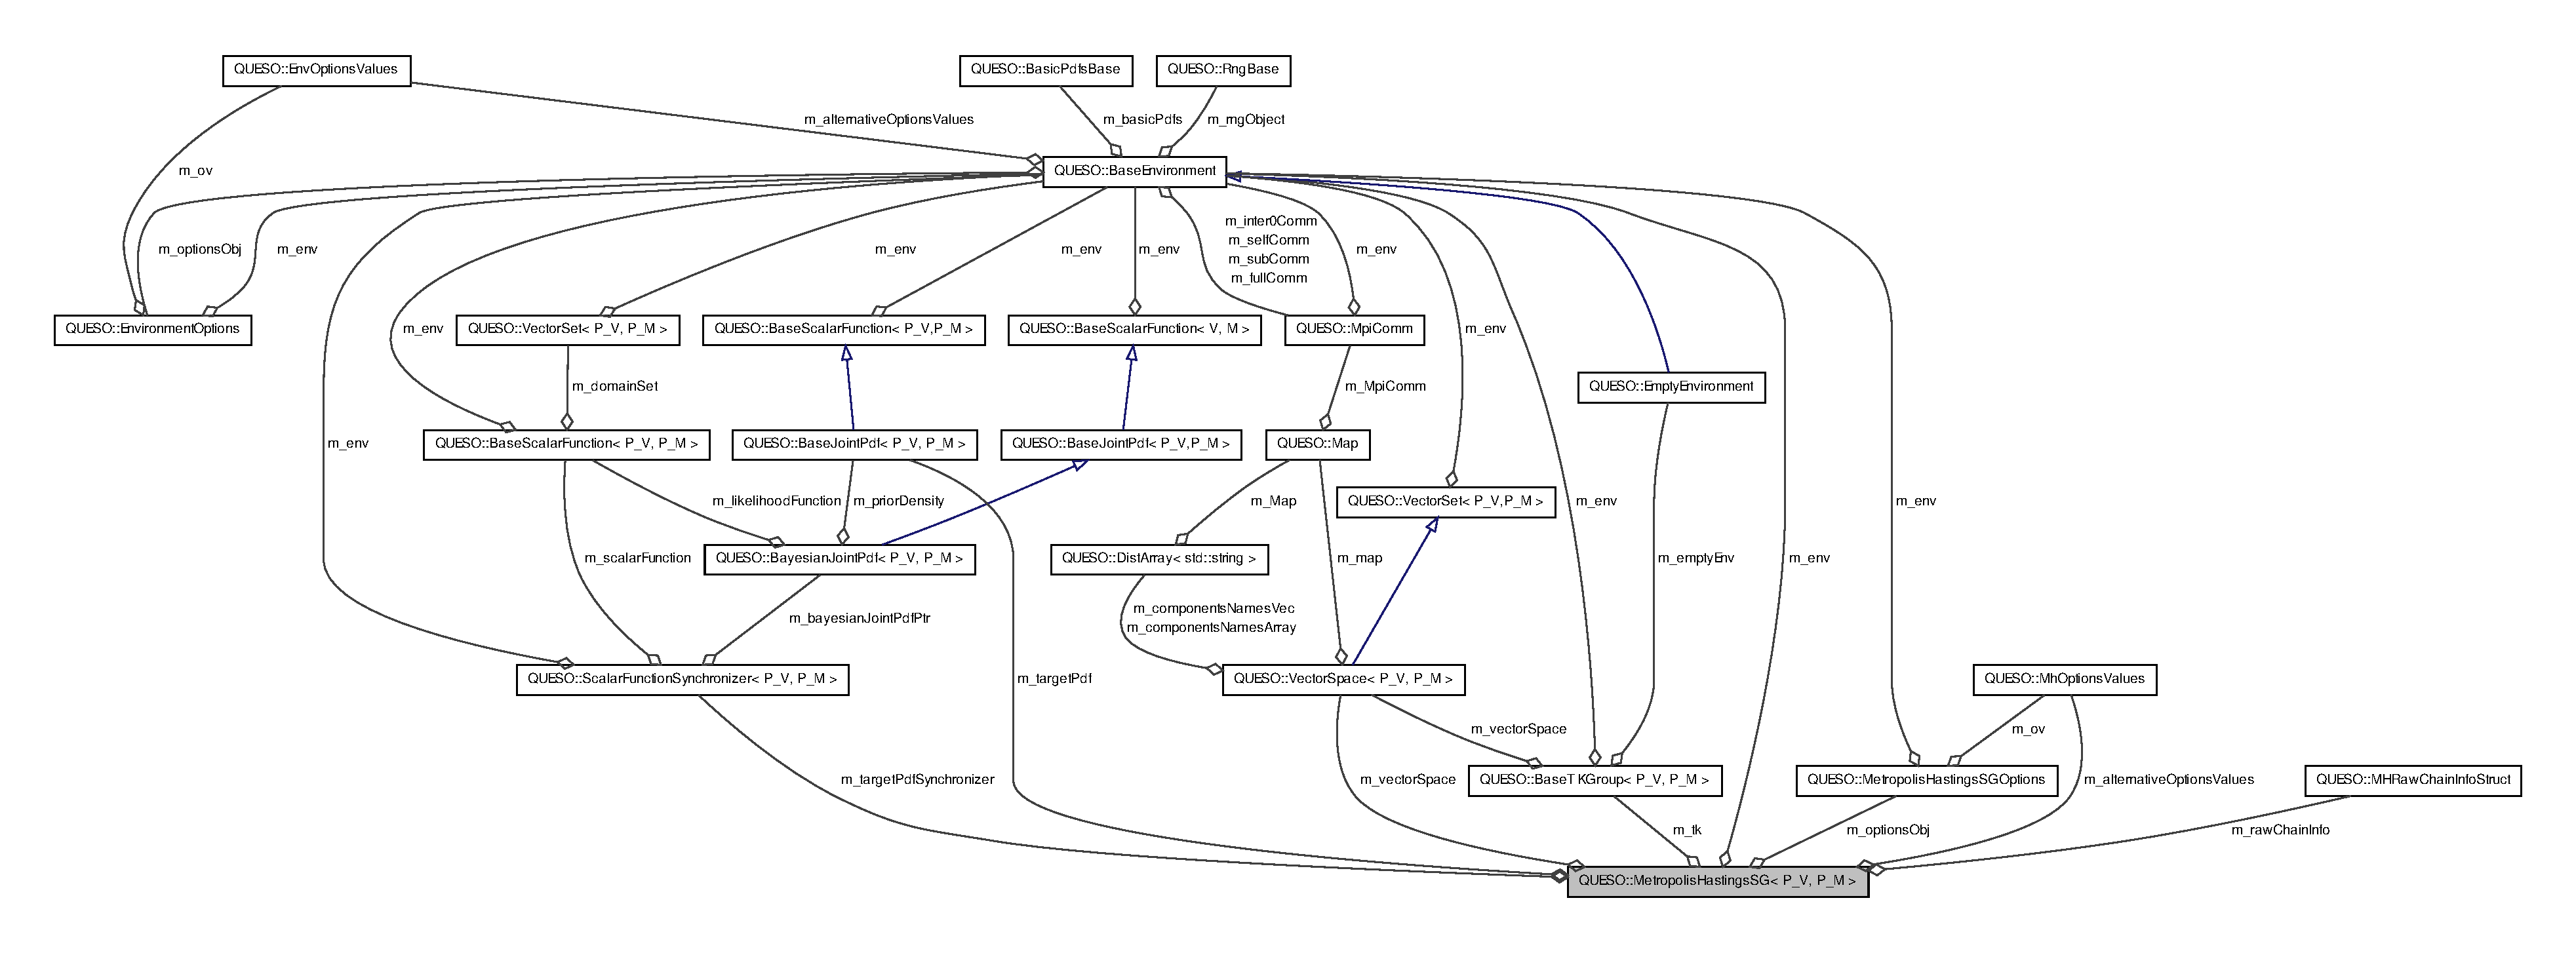
\includegraphics[scale=.35,clip=true,angle=90]{rawfigs/metropolis_hastings_coll}
 \vspace{-.8cm}
\caption{Collaboration graph of the  Metropolis-Hastings sequence generator class.}
\label{fig-metropolis-hastings-coll}
\end{figure}

\begin{table}[htpb]
\begin{center}
\caption{Input file options for a QUESO Metropolis-Hastings solver.}\label{tab-metropolis-hastings-options}
\vspace*{-8pt}
\ttfamily\footnotesize
\begin{tabular}{l c} %  m{4cm}}
\toprule
\rmfamily Option Name                                    & \rmfamily Default Value \\%& \rmfamily Description \\ %
\midrule\midrule
 \textlangle PREFIX\textrangle mh\_dataOutputFileName                       & "."   \\ % (UQ_MH_SG_DATA_OUTPUT_FILE_NAME_ODV),
 \textlangle PREFIX\textrangle mh\_dataOutputAllowAll                       & 0     \\ % (UQ_MH_SG_DATA_OUTPUT_ALLOW_ALL_ODV),
 \textlangle PREFIX\textrangle mh\_initialPositionDataInputFileName         & "."   \\ % (UQ_MH_SG_INITIAL_POSITION_DATA_INPUT_FILE_NAME_ODV),
 \textlangle PREFIX\textrangle mh\_initialPositionDataInputFileType         & "m"   \\ % (UQ_MH_SG_INITIAL_POSITION_DATA_INPUT_FILE_TYPE_ODV),
 \textlangle PREFIX\textrangle mh\_initialProposalCovMatrixDataInputFileName& "."   \\ % (UQ_MH_SG_INITIAL_PROPOSAL_COV_MATRIX_DATA_INPUT_FILE_NAME_ODV),
 \textlangle PREFIX\textrangle mh\_initialProposalCovMatrixDataInputFileType& "m"   \\ % (UQ_MH_SG_INITIAL_PROPOSAL_COV_MATRIX_DATA_INPUT_FILE_TYPE_ODV),
 \textlangle PREFIX\textrangle mh\_rawChainDataInputFileName                & "."   \\ % (UQ_MH_SG_RAW_CHAIN_DATA_INPUT_FILE_NAME_ODV),
 \textlangle PREFIX\textrangle mh\_rawChainDataInputFileType                & "m"   \\ % (UQ_MH_SG_RAW_CHAIN_DATA_INPUT_FILE_TYPE_ODV),
 \textlangle PREFIX\textrangle mh\_rawChainSize                             & 100   \\ % (UQ_MH_SG_RAW_CHAIN_SIZE_ODV),
 \textlangle PREFIX\textrangle mh\_rawChainGenerateExtra                    &  0    \\ % (UQ_MH_SG_RAW_CHAIN_GENERATE_EXTRA_ODV),
 \textlangle PREFIX\textrangle mh\_rawChainDisplayPeriod                    & 500   \\ % (UQ_MH_SG_RAW_CHAIN_DISPLAY_PERIOD_ODV),
 \textlangle PREFIX\textrangle mh\_rawChainMeasureRunTimes                  &  1    \\ % (UQ_MH_SG_RAW_CHAIN_MEASURE_RUN_TIMES_ODV),
 \textlangle PREFIX\textrangle mh\_rawChainDataOutputPeriod                 &  0    \\ % (UQ_MH_SG_RAW_CHAIN_DATA_OUTPUT_PERIOD_ODV),
 \textlangle PREFIX\textrangle mh\_rawChainDataOutputFileName               & "."   \\ % (UQ_MH_SG_RAW_CHAIN_DATA_OUTPUT_FILE_NAME_ODV),
 \textlangle PREFIX\textrangle mh\_rawChainDataOutputFileType               & "m"   \\ % (UQ_MH_SG_RAW_CHAIN_DATA_OUTPUT_FILE_TYPE_ODV),
 \textlangle PREFIX\textrangle mh\_rawChainDataOutputAllowAll               &  0    \\ % (UQ_MH_SG_RAW_CHAIN_DATA_OUTPUT_ALLOW_ALL_ODV),
 \textlangle PREFIX\textrangle mh\_filteredChainGenerate                    &  0    \\ % (UQ_MH_SG_FILTERED_CHAIN_GENERATE_ODV),
 \textlangle PREFIX\textrangle mh\_filteredChainDiscardedPortion            &  0.   \\ % (UQ_MH_SG_FILTERED_CHAIN_DISCARDED_PORTION_ODV),
 \textlangle PREFIX\textrangle mh\_filteredChainLag                         &  1    \\ % (UQ_MH_SG_FILTERED_CHAIN_LAG_ODV),
 \textlangle PREFIX\textrangle mh\_filteredChainDataOutputFileName          & "."   \\ % (UQ_MH_SG_FILTERED_CHAIN_DATA_OUTPUT_FILE_NAME_ODV),
 \textlangle PREFIX\textrangle mh\_filteredChainDataOutputFileType          & "m"   \\ % (UQ_MH_SG_FILTERED_CHAIN_DATA_OUTPUT_FILE_TYPE_ODV),
 \textlangle PREFIX\textrangle mh\_filteredChainDataOutputAllowAll          &  0   \\ % (UQ_MH_SG_FILTERED_CHAIN_DATA_OUTPUT_ALLOW_ALL_ODV),
 \textlangle PREFIX\textrangle mh\_displayCandidates                        &  0    \\ % (UQ_MH_SG_DISPLAY_CANDIDATES_ODV),
 \textlangle PREFIX\textrangle mh\_putOutOfBoundsInChain                    &  1    \\ % (UQ_MH_SG_PUT_OUT_OF_BOUNDS_IN_CHAIN_ODV),
 \textlangle PREFIX\textrangle mh\_tkUseLocalHessian                        &  0    \\ % (UQ_MH_SG_TK_USE_LOCAL_HESSIAN_ODV),
 \textlangle PREFIX\textrangle mh\_tkUseNewtonComponent                     &  1    \\ % (UQ_MH_SG_TK_USE_NEWTON_COMPONENT_ODV),
 \textlangle PREFIX\textrangle mh\_drMaxNumExtraStages                      &  0    \\ % (UQ_MH_SG_DR_MAX_NUM_EXTRA_STAGES_ODV),
%\textlangle PREFIX\textrangle mh\_drScalesForExtraStages                   &    \\ % (0),
 \textlangle PREFIX\textrangle mh\_drDuringAmNonAdaptiveInt                 &  1    \\ % (UQ_MH_SG_DR_DURING_AM_NON_ADAPTIVE_INT_ODV),
 \textlangle PREFIX\textrangle mh\_amKeepInitialMatrix                      &  0    \\ % (UQ_MH_SG_AM_KEEP_INITIAL_MATRIX_ODV),
 \textlangle PREFIX\textrangle mh\_amInitialNonAdaptInterval                &  0    \\ % (UQ_MH_SG_AM_INIT_NON_ADAPT_INT_ODV),
 \textlangle PREFIX\textrangle mh\_amAdaptInterval                          &  0    \\ % (UQ_MH_SG_AM_ADAPT_INTERVAL_ODV),
 \textlangle PREFIX\textrangle mh\_amAdaptedMatricesDataOutputPeriod        &  0    \\ % (UQ_MH_SG_AM_ADAPTED_MATRICES_DATA_OUTPUT_PERIOD_ODV),
 \textlangle PREFIX\textrangle mh\_amAdaptedMatricesDataOutputFileName      & "."   \\ % (UQ_MH_SG_AM_ADAPTED_MATRICES_DATA_OUTPUT_FILE_NAME_ODV),
 \textlangle PREFIX\textrangle mh\_amAdaptedMatricesDataOutputFileType      & "m"   \\ % (UQ_MH_SG_AM_ADAPTED_MATRICES_DATA_OUTPUT_FILE_TYPE_ODV),
 \textlangle PREFIX\textrangle mh\_amAdaptedMatricesDataOutputAllowAll      &  0    \\ % (UQ_MH_SG_AM_ADAPTED_MATRICES_DATA_OUTPUT_ALLOW_ALL_ODV),
%\textlangle PREFIX\textrangle mh\_amAdaptedMatricesDataOutputAllowedSet    &    \\ % (),
 \textlangle PREFIX\textrangle mh\_amEta                                    & 1.    \\ % (UQ_MH_SG_AM_ETA_ODV),
 \textlangle PREFIX\textrangle mh\_amEpsilon                                & $1\times 10^{-5}$   \\ % (UQ_MH_SG_AM_EPSILON_ODV),
 \textlangle PREFIX\textrangle mh\_enableBrooksGelmanConvMonitor            & 0    \\ % (UQ_MH_SG_ENABLE_BROOKS_GELMAN_CONV_MONITOR),
 \textlangle PREFIX\textrangle mh\_BrooksGelmanLag                          & 100   \\ % (UQ_MH_SG_BROOKS_GELMAN_LAG)
\bottomrule
\end{tabular}
\end{center}
\end{table}




%\clearpage
\subsection{Multilevel Solver (and Options)}\label{sec:ML}


The templated class that represents a Multilevel generator of samples in QUESO is \linebreak \verb+MLSampling<P_V,P_M>+. This class implements the Adaptive Multilevel Stochastic Simulation Algorithm of Cheung and Prudencio~\cite{CheungPrudencio2012}.
The Multilevel sequence generator class is assisted by two extra classes, \verb+MLSamplingOptions+ and \verb+MLSamplingLevelOptions+, for handling the options to be used.

The Multilevel class, the Multilevel options and level options classes are depicted in Figure~\ref{fig-Multilevel-options-class}.  A collaboration graph for the Multilevel class is presented in Figure \ref{fig-Multilevel-coll}; whereas its associated options are presented in Table \ref{tab-Multilevel-options}.
% 
% \begin{figure}[htpb]
% \centering
% 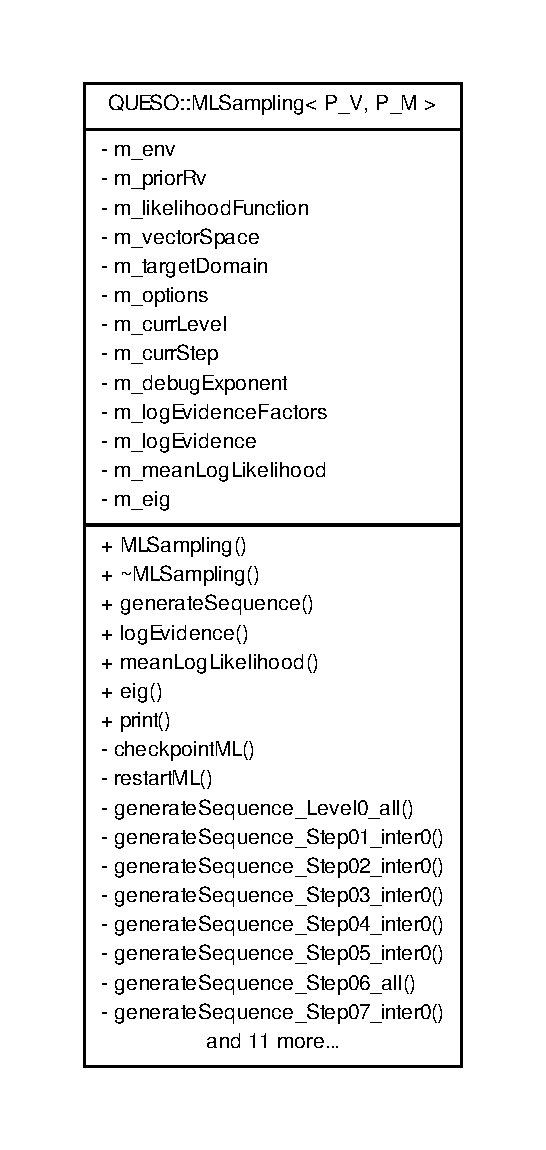
\includegraphics[scale=0.8,clip=true]{rawfigs/ml_sampling}
% \vspace{-1.cm}
% \caption{The Multilevel sequence generator class.}
% \label{fig-Multilevel-solver-class}
% \end{figure}

\begin{figure}[htpb]
\centering
\subfloat[MLSampling]{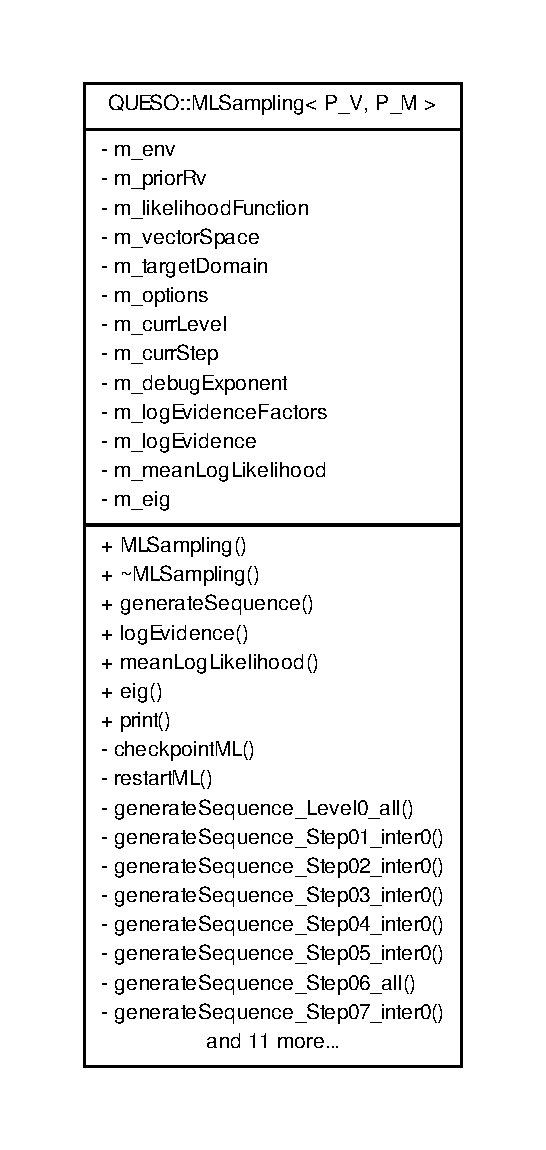
\includegraphics[trim={0 1.3cm 0 0},clip,scale=0.65]{rawfigs/ml_sampling}\label{fig-Multilevel-solver-class}}\hspace{-1.5cm}
\subfloat[MLSamplingOptions]{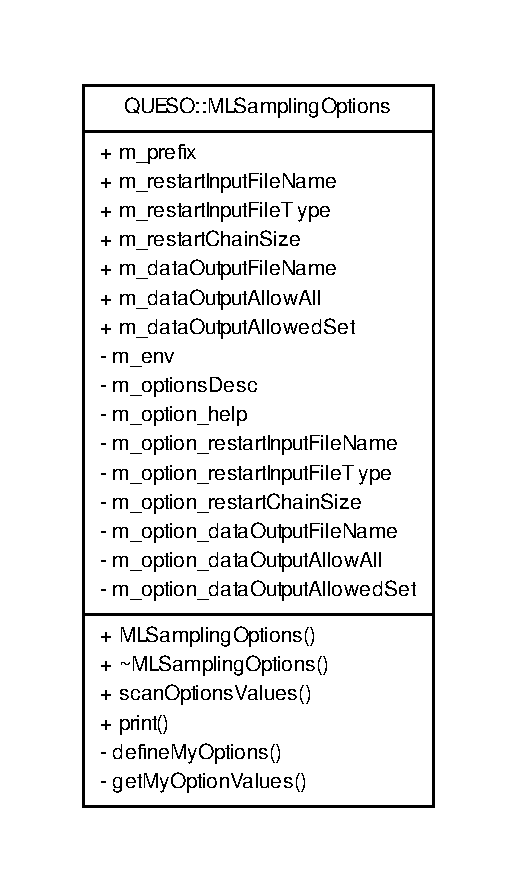
\includegraphics[trim={0 1.3cm 0 0},clip,scale=0.65]{rawfigs/ml_sampling_options}}\hspace{-1.5cm}
\subfloat[MLSamplingLevelOptions]{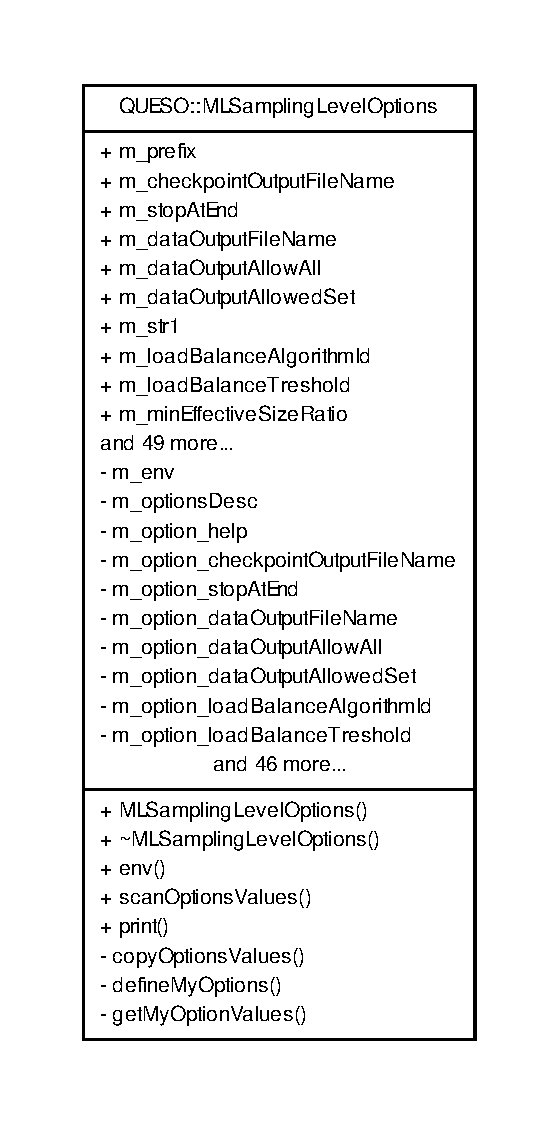
\includegraphics[trim={0 1.3cm 0 0},clip,scale=0.65]{rawfigs/ml_sampling_level_options}}
 \vspace{-.2cm}
\caption{The Multilevel sequence generator options class (\ref{fig-Multilevel-solver-class}) and its associated classes for handling options.}
\label{fig-Multilevel-options-class}
\end{figure}


\begin{figure}[p]
\centering
% 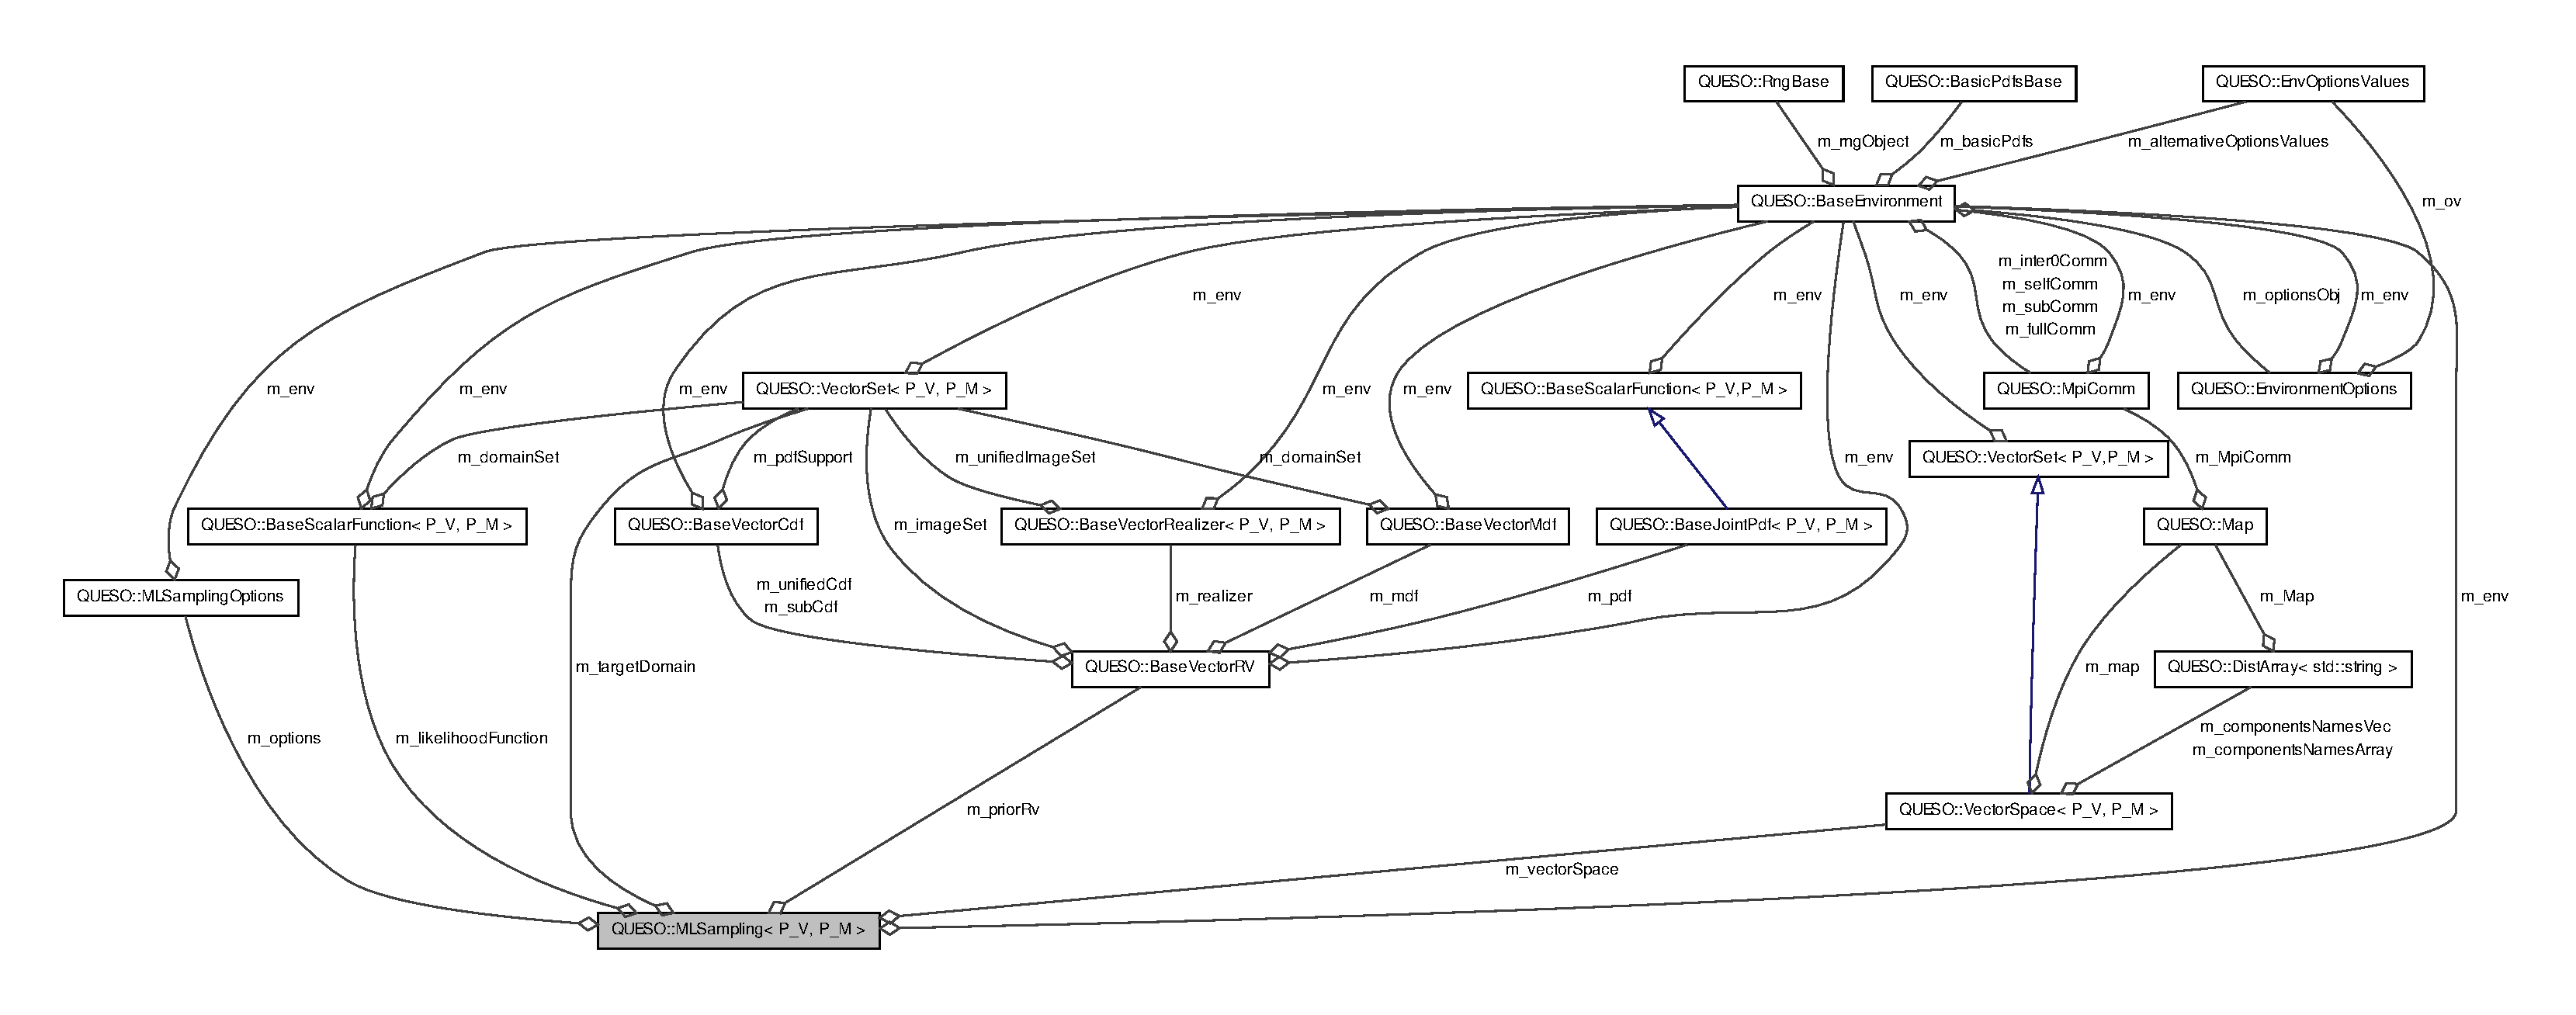
\includegraphics[width=1.3\textwidth, height=.7\textheight,clip=true,angle=90]{rawfigs/ml_coll}
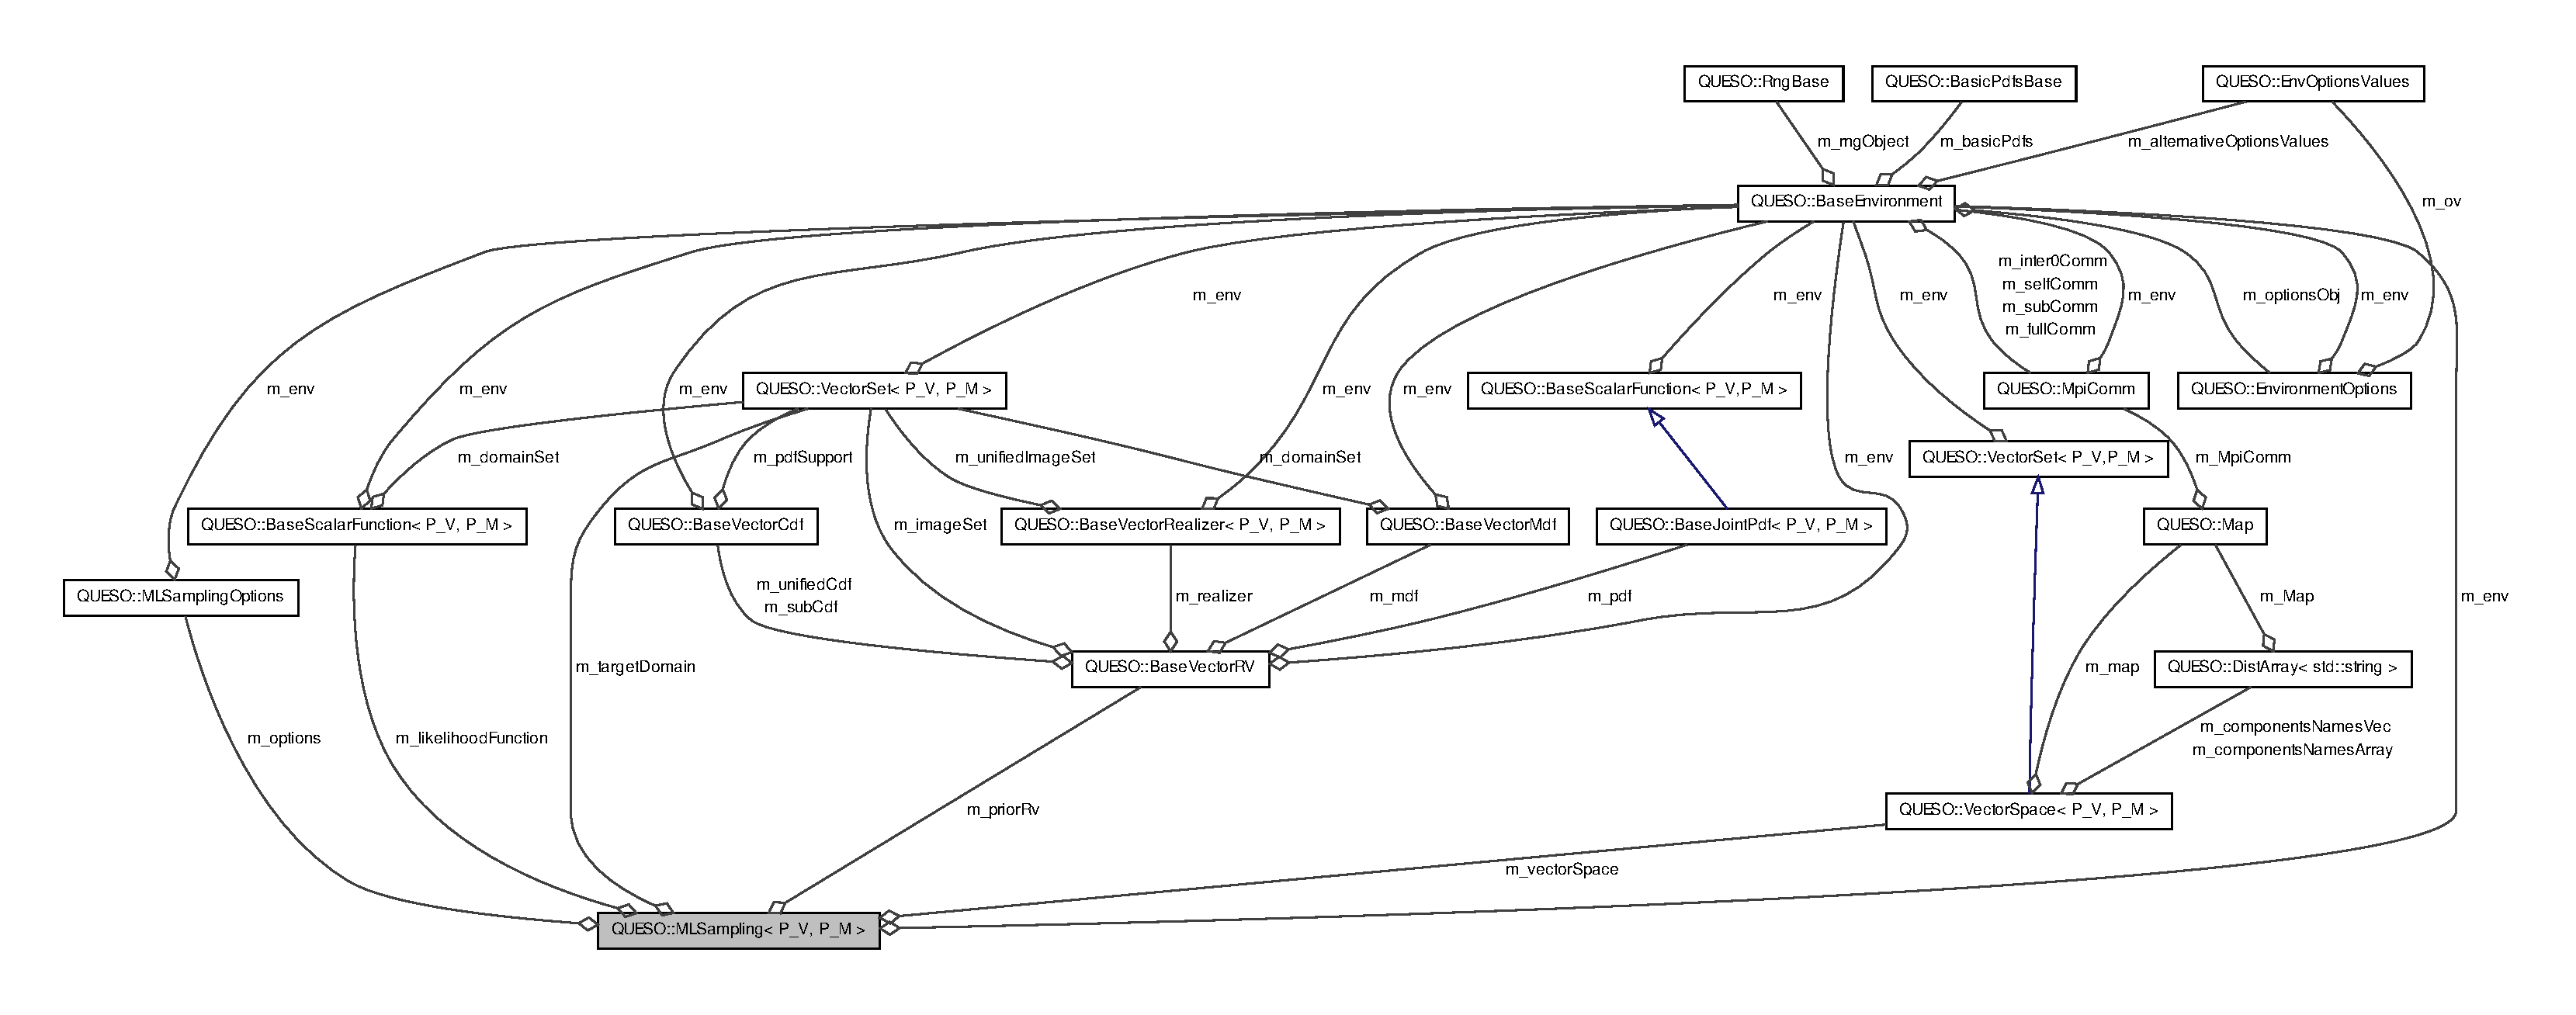
\includegraphics[scale=.4,clip=true,angle=90]{rawfigs/ml_coll}
 \vspace{-.8cm}
\caption{Collaboration graph of the  Multilevel sampling class.}
\label{fig-Multilevel-coll}
\end{figure}


\begin{table}[p]
\begin{center}
\caption{Input file options for a QUESO Multilevel solver (to be continued).}\label{tab-Multilevel-options}
\vspace*{-8pt}
\ttfamily\footnotesize
\begin{tabular}{l c} %  m{4cm}}
\toprule
\rmfamily Option Name                                    & \rmfamily Default Value \\%& \rmfamily Description \\ %
\midrule\midrule
% \textlangle PREFIX\textrangle
% ml\_dataOutputFileName              & "."  \\ %  (UQ_ML_SAMPLING_DATA_Output\_FILE_NAME_ODV  )

\textlangle PREFIX\textrangle
ml\_restartOutput\_levelPeriod       & 0    \\ %  (UQ_ML_SAMPLING_RESTART_Output\_LEVEL_PERIOD_ODV       ),

\textlangle PREFIX\textrangle 
ml\_restartOutput\_baseNameForFiles  & "."  \\ %  (UQ_ML_SAMPLING_RESTART_Output\_BASE_NAME_FOR_FILES_ODV),

\textlangle PREFIX\textrangle 
ml\_restartOutput\_fileType          & "m"  \\ %  (UQ_ML_SAMPLING_RESTART_Output\_FILE_TYPE_ODV          ),

\textlangle PREFIX\textrangle 
ml\_restartInput\_baseNameForFiles   & "."  \\ %  (UQ_ML_SAMPLING_RESTART_Input\_BASE_NAME_FOR_FILES_ODV ),

\textlangle PREFIX\textrangle 
ml\_restartInput\_fileType           & "m"  \\ %  (UQ_ML_SAMPLING_RESTART_Input\_FILE_TYPE_ODV           ),

% \textlangle PREFIX\textrangle ml\_option\_dataOutputAllowedSet   & ""  \\ %  (\textlangle PREFIX\textrangle ml\_prefix + "dataOutputAllowedSet")

 \textlangle PREFIX\textrangle ml\_stopAtEnd                                 & 0    \\%  (UQ_ML_SAMPLING_L_STOP_AT_END_ODV),
 \textlangle PREFIX\textrangle ml\_dataOutputFileName                        & "."  \\%  (UQ_ML_SAMPLING_L_DATA_OUTPUT_FILE_NAME_ODV),
 \textlangle PREFIX\textrangle ml\_dataOutputAllowAll                        & 0    \\%  (UQ_ML_SAMPLING_L_DATA_OUTPUT_ALLOW_ALL_ODV),
 \textlangle PREFIX\textrangle ml\_loadBalanceAlgorithmId                    & 2    \\%  (UQ_ML_SAMPLING_L_LOAD_BALANCE_ALGORITH),
 \textlangle PREFIX\textrangle ml\_loadBalanceTreshold                       & 1.0  \\%  (UQ_ML_SAMPLING_L_LOAD_BALANCE_TRESHOLD_ODV),
 \textlangle PREFIX\textrangle ml\_minEffectiveSizeRatio                     & 0.85 \\%  (UQ_ML_SAMPLING_L_MIN_EFFECTIVE_SIZE_RATIO_ODV),
 \textlangle PREFIX\textrangle ml\_maxEffectiveSizeRatio                     & 0.91 \\%  (UQ_ML_SAMPLING_L_MAX_EFFECTIVE_SIZE_RATIO_ODV),
 \textlangle PREFIX\textrangle ml\_scaleCovMatrix                            & 1    \\%  (UQ_ML_SAMPLING_L_SCALE_COV_MATRIX_ODV),
 \textlangle PREFIX\textrangle ml\_minRejectionRate                          & 0.50 \\%  (UQ_ML_SAMPLING_L_MIN_REJECTION_RATE_ODV),
 \textlangle PREFIX\textrangle ml\_maxRejectionRate                          & 0.75 \\%  (UQ_ML_SAMPLING_L_MAX_REJECTION_RATE_ODV),
 \textlangle PREFIX\textrangle ml\_covRejectionRate                          & 0.25 \\%  (UQ_ML_SAMPLING_L_COV_REJECTION_RATE_ODV),
 \textlangle PREFIX\textrangle ml\_minAcceptableEta                          & 0.   \\%  (UQ_ML_SAMPLING_L_MIN_ACCEPTABLE_ETA_ODV), // gpmsa
 \textlangle PREFIX\textrangle ml\_totallyMute                               & 1    \\%  (UQ_ML_SAMPLING_L_TOTALLY_MUTE_ODV),
 \textlangle PREFIX\textrangle ml\_initialPositionDataInputFileName          & "."  \\%  (UQ_ML_SAMPLING_L_INITIAL_POSITION_DATA_INPUT_FILE_NAME_ODV),
 \textlangle PREFIX\textrangle ml\_initialPositionDataInputFileType          & "m"  \\%  (UQ_ML_SAMPLING_L_INITIAL_POSITION_DATA_INPUT_FILE_TYPE_ODV),
 \textlangle PREFIX\textrangle ml\_initialProposalCovMatrixDataInputFileName & "."  \\%  (UQ_ML_SAMPLING_L_INITIAL_PROPOSAL_COV_MATRIX_DATA_INPUT_FILE_NAME_ODV),
 \textlangle PREFIX\textrangle ml\_initialProposalCovMatrixDataInputFileType & "m"  \\%  (UQ_ML_SAMPLING_L_INITIAL_PROPOSAL_COV_MATRIX_DATA_INPUT_FILE_TYPE_ODV),
 \textlangle PREFIX\textrangle ml\_rawChainDataInputFileName                 & "."  \\%  (UQ_ML_SAMPLING_L_RAW_CHAIN_DATA_INPUT_FILE_NAME_ODV),
 \textlangle PREFIX\textrangle ml\_rawChainDataInputFileType                 & "m"  \\%  (UQ_ML_SAMPLING_L_RAW_CHAIN_DATA_INPUT_FILE_TYPE_ODV),
 \textlangle PREFIX\textrangle ml\_rawChainSize                              & 100  \\%  (UQ_ML_SAMPLING_L_RAW_CHAIN_SIZE_ODV),
 \textlangle PREFIX\textrangle ml\_rawChainGenerateExtra                     & 0    \\%  (UQ_ML_SAMPLING_L_RAW_CHAIN_GENERATE_EXTRA_ODV),
 \textlangle PREFIX\textrangle ml\_rawChainDisplayPeriod                     & 500  \\%  (UQ_ML_SAMPLING_L_RAW_CHAIN_DISPLAY_PERIOD_ODV),
 \textlangle PREFIX\textrangle ml\_rawChainMeasureRunTimes                   & 1    \\%  (UQ_ML_SAMPLING_L_RAW_CHAIN_MEASURE_RUN_TIMES_ODV),
 \textlangle PREFIX\textrangle ml\_rawChainDataOutputPeriod                  & 0    \\%  (UQ_ML_SAMPLING_L_RAW_CHAIN_DATA_OUTPUT_PERIOD_ODV),
 \textlangle PREFIX\textrangle ml\_rawChainDataOutputFileName                & "."  \\%  (UQ_ML_SAMPLING_L_RAW_CHAIN_DATA_OUTPUT_FILE_NAME_ODV),
 \textlangle PREFIX\textrangle ml\_rawChainDataOutputFileType                & "m"  \\%  (UQ_ML_SAMPLING_L_RAW_CHAIN_DATA_OUTPUT_FILE_TYPE_ODV),
 \textlangle PREFIX\textrangle ml\_rawChainDataOutputAllowAll                & 0    \\%  (UQ_ML_SAMPLING_L_RAW_CHAIN_DATA_OUTPUT_ALLOW_ALL_ODV),
 \textlangle PREFIX\textrangle ml\_filteredChainGenerate                     & 0    \\%  (UQ_ML_SAMPLING_L_FILTERED_CHAIN_GENERATE_ODV),
 \textlangle PREFIX\textrangle ml\_filteredChainDiscardedPortion             & 0.   \\%  (UQ_ML_SAMPLING_L_FILTERED_CHAIN_DISCARDED_PORTION_ODV),
 \textlangle PREFIX\textrangle ml\_filteredChainLag                          & 1    \\%  (UQ_ML_SAMPLING_L_FILTERED_CHAIN_LAG_ODV),
 \textlangle PREFIX\textrangle ml\_filteredChainDataOutputFileName           & "."  \\%  (UQ_ML_SAMPLING_L_FILTERED_CHAIN_DATA_OUTPUT_FILE_NAME_ODV),
 \textlangle PREFIX\textrangle ml\_filteredChainDataOutputFileType           & "m"  \\%  (UQ_ML_SAMPLING_L_FILTERED_CHAIN_DATA_OUTPUT_FILE_TYPE_ODV),
 \textlangle PREFIX\textrangle ml\_filteredChainDataOutputAllowAll           & 0    \\%  (UQ_ML_SAMPLING_L_FILTERED_CHAIN_DATA_OUTPUT_ALLOW_ALL_ODV),
 \textlangle PREFIX\textrangle ml\_displayCandidates                         & 0    \\%  (UQ_ML_SAMPLING_L_DISPLAY_CANDIDATES_ODV),
 \textlangle PREFIX\textrangle ml\_putOutOfBoundsInChain                     & 1    \\%  (UQ_ML_SAMPLING_L_PUT_OUT_OF_BOUNDS_IN_CHAIN_ODV),

 \textlangle PREFIX\textrangle ml\_tkUseLocalHessian                         & 0    \\%  (UQ_ML_SAMPLING_L_TK_USE_LOCAL_HESSIAN_ODV),
 \textlangle PREFIX\textrangle ml\_tkUseNewtonComponent                      & 1    \\%  (UQ_ML_SAMPLING_L_TK_USE_NEWTON_COMPONENT_ODV),
 \textlangle PREFIX\textrangle ml\_drMaxNumExtraStages                       & 0    \\%  (UQ_ML_SAMPLING_L_DR_MAX_NUM_EXTRA_STAGES_ODV),
 \textlangle PREFIX\textrangle ml\_drScalesForExtraStages                    & 0    \\%  (0),
 \textlangle PREFIX\textrangle ml\_drDuringAmNonAdaptiveInt                  & 1    \\%  (UQ_ML_SAMPLING_L_DR_DURING_AM_NON_ADAPTIVE_INT_ODV),
 \textlangle PREFIX\textrangle ml\_amKeepInitialMatrix                       & 0    \\%  (UQ_ML_SAMPLING_L_AM_KEEP_INITIAL_MATRIX_ODV),
 \textlangle PREFIX\textrangle ml\_amInitialNonAdaptInterval                 & 0    \\%  (UQ_ML_SAMPLING_L_AM_INIT_NON_ADAPT_INT_ODV),
 \textlangle PREFIX\textrangle ml\_amAdaptInterval                           & 0    \\%  (UQ_ML_SAMPLING_L_AM_ADAPT_INTERVAL_ODV),
 \textlangle PREFIX\textrangle ml\_amAdaptedMatricesDataOutputPeriod         & 0    \\%  (UQ_ML_SAMPLING_L_AM_ADAPTED_MATRICES_DATA_OUTPUT_PERIOD_ODV),
 \textlangle PREFIX\textrangle ml\_amAdaptedMatricesDataOutputFileName       & "."  \\ %  (UQ_ML_SAMPLING_L_AM_ADAPTED_MATRICES_DATA_OUTPUT_FILE_NAME_ODV),
 \textlangle PREFIX\textrangle ml\_amAdaptedMatricesDataOutputFileType       & "m"  \\ %  (UQ_ML_SAMPLING_L_AM_ADAPTED_MATRICES_DATA_OUTPUT_FILE_TYPE_ODV),
 \textlangle PREFIX\textrangle ml\_amAdaptedMatricesDataOutputAllowAll       & 0    \\ %  (UQ_ML_SAMPLING_L_AM_ADAPTED_MATRICES_DATA_OUTPUT_ALLOW_ALL_ODV),
 \textlangle PREFIX\textrangle ml\_amEta                                     & 1.   \\ %  (UQ_ML_SAMPLING_L_AM_ETA_ODV),
 \textlangle PREFIX\textrangle ml\_amEpsilon                                 & 1.e-5\\ %  (UQ_ML_SAMPLING_L_AM_EPSILON_ODV),
\bottomrule
\end{tabular}
\end{center}
\end{table}



% 
% \begin{table}[!p]
% \begin{center}
% \caption{Input file options for a QUESO Multilevel solver (continuation of Table \ref{tab-Multilevel-options}).}
% %\vspace*{-8pt}
% \ttfamily\small
% \begin{tabular}{l c} %  m{4cm}}
% \toprule
% \rmfamily Option Name                                    & \rmfamily Default Value \\%& \rmfamily Description \\ %
% \midrule\midrule
% 
% 
% \bottomrule
% \end{tabular}
% \end{center}
% \end{table}


%\clearpage
\subsection{Statistical Forward Problem (and Options)}

A SFP in QUESO also has two input entities, the input (parameter) RV and a QoI function, and one output entity, the QoI RV. 
The SIP is represented through the templated class \verb+StatisticalForwardProblem<P_V,P_M,Q_V,Q_M >+, which diagram is presented in Figure \ref{fig-sfp-class}. Again, the types \verb+P_V+ and \verb+Q_V+ of vectors and types \verb+P_M+ and \verb+Q_M+ of matrices, where \verb+P_+ stands for 'parameter' and \verb+Q_+ stands for 'quantities of interest'.

The input RV and the output QoI RV are instances of the \verb+BaseVectorRv<P_V,P_M>+ class, while
the QoI function is an instance of \verb+BaseVectorFunction<P_V,P_M,Q_V,Q_M>+.
In the template parameters, the prefix \verb+P_+ refers to the parameters, whereas the prefix \verb+Q_+ refers to the QoIs.

In order to find the solution of a SFP, one must call the \verb+solveWithMonteCarlo()+ member function of the \verb+StatisticalForwardProblem<P_V,P_M>+ class.
Upon return from a solution operation, the QoI RV is available through the \verb+qoiRv()+ member function. Such QoI RV  is able to provide:
a vector realizer through the operation \verb+'qoiRv().realizer()'+, which returns an instance of the class \verb+'uqBaseVectorRealizer<Q_V,Q_M>'+.



Figure \ref{fig-sfp-options-class} displays the  statistical forward problem options class, i.e. that class that handles a variety of options for solving the SFP. Such options may be provided to QUESO at the user's input file; and they are listed in Table \ref{tab-sfp-options}. In the table, \texttt{p-q} stands for parameter--quantity of interest. 



 
%it provides both CDFs of QoI components through the operation \verb+qoiRv().unifiedCdf()+,  which returns an instance of the class \verb+BaseVectorCdf<Q_V,Q_M>+, and
%a vector realizer through the operation \verb+qoiRv().realizer()+, which returns an instance of the class \verb+BaseVectorRealizer<Q_V,Q_M>+.

\begin{figure}[p]
\centering
\centering
\subfloat[StatisticalForwardProblem]{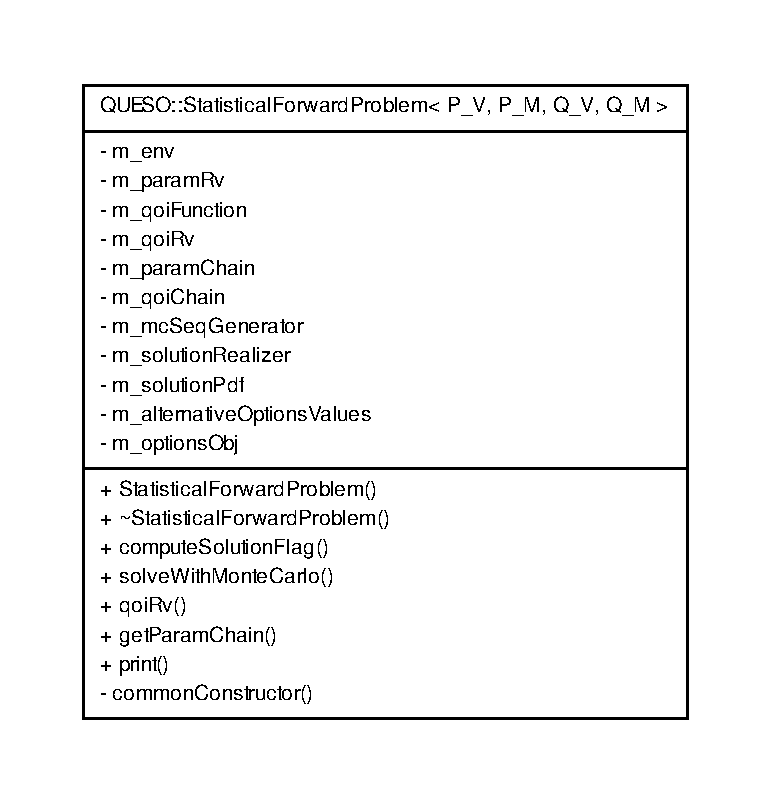
\includegraphics[trim={0.5cm 1.3cm 0 0},clip,scale=0.7]{rawfigs/statistical_forward_problem}\label{fig-sfp-class}}
%
\subfloat[StatisticalForwardProblemOptions]{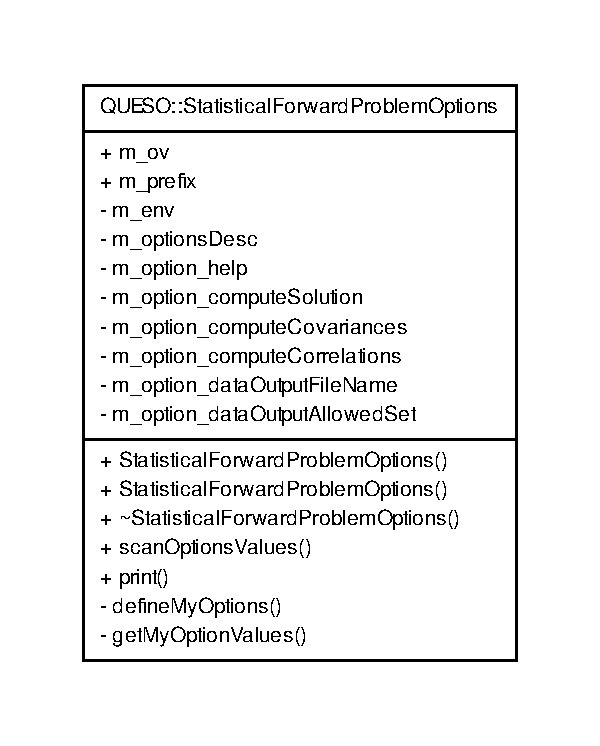
\includegraphics[trim={0.5cm 1.3cm 0 0},clip,scale=0.7]{rawfigs/statistical_forward_problem_options}\label{fig-sfp-options-class}}
\vspace{-.2cm}
%
\caption{The statistical forward problem class, which implements the representation in Figure~\ref{fig-sfp-queso}, and the statistical forward problem options class.}
\end{figure}




\begin{table}[htpb]
% from uqStatisticalForwardProblemOptions.C and .h
\caption{Input file options for a QUESO statistical forward problem.}\label{tab-sfp-options}
\vspace{-8pt}
\ttfamily\footnotesize
\begin{center}
\begin{tabular}{l c  m{6cm}}
\toprule
 \rmfamily Option Name                     & \rmfamily Default Value& \rmfamily Description \\
\midrule
%\textlangle PREFIX\textrangle fp\_help                 &       &             \\ %
%\hline
\textlangle PREFIX\textrangle fp\_computeSolution      &   1  &\rmfamily Computes the solution process   \\%UQ_SFP_COMPUTE_SOLUTION_ODV
%\hline
\textlangle PREFIX\textrangle fp\_computeCovariances   &   1  &\rmfamily Compute \verb+p-q+ covariances    \\ %UQ_SFP_COMPUTE_COVARIANCES_ODV
%\hline
\textlangle PREFIX\textrangle fp\_computeCorrelations  &   1  &\rmfamily Compute \verb+p-q+ correlations   \\ %UQ_SFP_COMPUTE_CORRELATIONS_ODV
%\hline
\textlangle PREFIX\textrangle fp\_dataOutputFileName   &  "." &\rmfamily Name of data output file  \\ %UQ_SFP_DATA_OUTPUT_FILE_NAME_ODV
%\hline
\textlangle PREFIX\textrangle fp\_dataOutputAllowedSet &  ""  &\rmfamily Subenvironments that will write to data output file   \\ %UQ_SFP_DATA_OUTPUT_ALLOWED_SET_ODV
\bottomrule
\end{tabular}
\end{center}
\end{table}

%\clearpage
\subsection{Monte Carlo Solver (and Options)}

The templated class that implements a Monte Carlo generator of samples within QUESO is \verb+MonteCarloSG<P_V,P_M,Q_V,Q_M>+, as illustrated in Figure \ref{fig-monte-carlo-solver-class}.
This class has the requirement that the image set of the vector random variable  and the domain set of the QoI function belong to vector spaces of equal dimensions. If the requirements are satisfied, the class constructor reads input options that begin with the string `\verb+<PREFIX>_mc_+' (See Table~\ref{tab-monte-carlo-options}). Options reading is handled by class \verb+MonteCarloOptions+, which is illustrated in Figure~\ref{fig-monte-carlo-options-class}.


\begin{figure}[p]
\centering
\subfloat[MonteCarloSG]{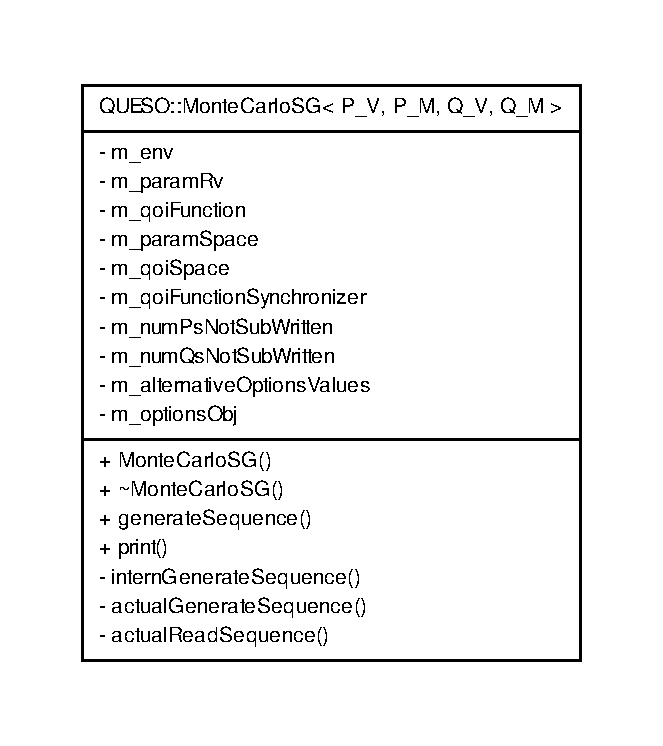
\includegraphics[trim={0.5cm 1.3cm 0 0},clip,scale=0.7]{rawfigs/monte_carlo}\label{fig-monte-carlo-solver-class}}
\subfloat[MonteCarloSGOptions]{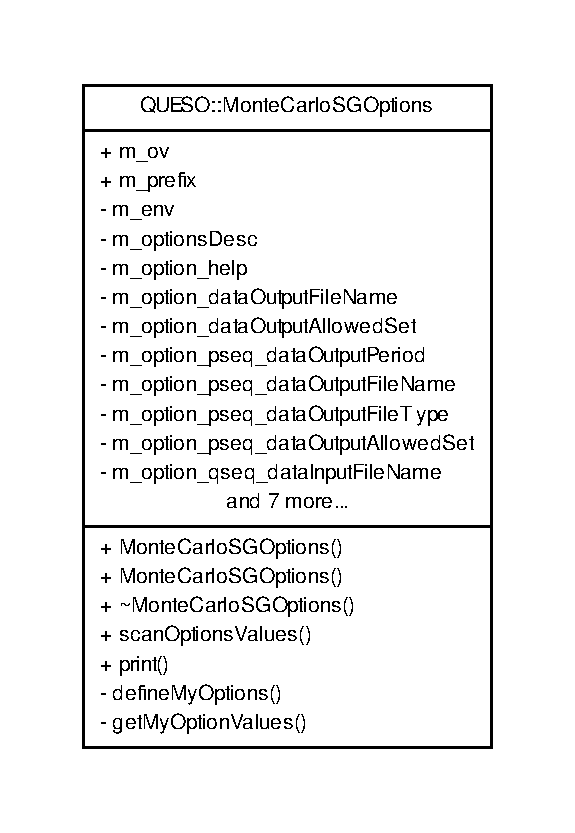
\includegraphics[trim={0.5cm 1.3cm 0 0},clip,scale=0.7]{rawfigs/monte_carlo_options}\label{fig-monte-carlo-options-class}}
\vspace*{-.2cm}
\caption{The Monte Carlo sequence generator class and the Monte Carlo sequence generator options class.}
\end{figure}



\begin{table}[htpb]
% from uqMonteCarloSGOptions.C and uqMonteCarloSGOptions.h
\begin{center}
\caption{Input file options for a QUESO statistical forward problem solved via Monte Carlo algorithm.}
\vspace{-8pt}
\label{tab-monte-carlo-options}
\ttfamily\footnotesize
\begin{tabular}{l c  m{6cm}}
\toprule
\rmfamily Option Name     & \rmfamily Default Value \\
\midrule\midrule
\textlangle PREFIX\textrangle mc\_dataOutputFileName           &  "."  \\
\textlangle PREFIX\textrangle mc\_dataOutputAllowedSet         &       \\
\textlangle PREFIX\textrangle mc\_pseq\_dataOutputFileName     &  "."  \\
\textlangle PREFIX\textrangle mc\_pseq\_dataOutputAllowedSet   &       \\
\textlangle PREFIX\textrangle mc\_qseq\_dataInputFileName      &  "."  \\
\textlangle PREFIX\textrangle mc\_qseq\_size                   &  100  \\
\textlangle PREFIX\textrangle mc\_qseq\_displayPeriod          &  500  \\  
\textlangle PREFIX\textrangle mc\_qseq\_measureRunTimes        &    0  \\  
\textlangle PREFIX\textrangle mc\_qseq\_dataOutputFileName     &  "."  \\ 
\textlangle PREFIX\textrangle mc\_qseq\_dataOutputAllowedSet   &       \\  
\bottomrule
\end{tabular}
\end{center}
\end{table}

% 
% \begin{table}[htpb]
% % from uqMonteCarloSGOptions.C and uqMonteCarloSGOptions.h
% \begin{center}
% \caption{Input file options for a QUESO statistical forward problem solved via Monte Carlo algorithm.}
% \vspace{-8pt}
% \label{tab-monte-carlo-options}
% \ttfamily
% \begin{tabular}{l c  m{6cm}}
% \toprule
% \rmfamily Option Name     & \rmfamily Default Value &  \rmfamily Description \\ %
% \midrule\midrule
% %\textlangle PREFIX\textrangle mc\_help                        &         &             \\ %_ODV = option default value
% %\hline
% \textlangle PREFIX\textrangle mc\_dataOutputFileName           &   "."   &             \\ % m_dataOutputFileName         (UQ_MOC_SG_DATA_OUTPUT_FILE_NAME_ODV 
% %\hline
% \textlangle PREFIX\textrangle mc\_dataOutputAllowedSet         &         &             \\ %//m_dataOutputAllowedSet       (),
% %\hline
% \textlangle PREFIX\textrangle mc\_pseq\_dataOutputFileName     &    "."  &             \\ %m_pseqDataOutputFileName     (UQ_MOC_SG_PSEQ_DATA_OUTPUT_FILE_NAME_ODV
% %\hline
% \textlangle PREFIX\textrangle mc\_pseq\_dataOutputAllowedSet   &         &             \\ %//m_pseqDataOutputAllowedSet   (),
% %\hline
% %\textlangle PREFIX\textrangle mc\_pseq\_computeStats           &         &             \\ %
% % \hline
% \textlangle PREFIX\textrangle mc\_qseq\_dataInputFileName      &   "."   &             \\ %m_qseqDataInputFileName      (UQ_MOC_SG_QSEQ_DATA_INPUT_FILE_NAME_ODV ),
% % \hline
% \textlangle PREFIX\textrangle mc\_qseq\_size                   &   100   &             \\ %m_qseqSize                   (UQ_MOC_SG_QSEQ_SIZE_ODV
% % \hline
% \textlangle PREFIX\textrangle mc\_qseq\_displayPeriod          &  500    &             \\ %m_qseqDisplayPeriod          (UQ_MOC_SG_QSEQ_DISPLAY_PERIOD_ODV
% % \hline
% \textlangle PREFIX\textrangle mc\_qseq\_measureRunTimes        &    0    &             \\ %m_qseqMeasureRunTimes        (UQ_MOC_SG_QSEQ_MEASURE_RUN_TIMES_ODV
% % \hline
% \textlangle PREFIX\textrangle mc\_qseq\_dataOutputFileName     &   "."   &             \\ %m_qseqDataOutputFileName     (UQ_MOC_SG_QSEQ_DATA_OUTPUT_FILE_NAME_ODV),
% % \hline
% \textlangle PREFIX\textrangle mc\_qseq\_dataOutputAllowedSet   &         &             \\ %//m_qseqDataOutputAllowedSet   (),
% % \hline
% %\textlangle PREFIX\textrangle mc\_qseq\_computeStats           &         &             \\ %
% \bottomrule
% \end{tabular}
% \end{center}
% \end{table}



% %\clearpage
% \subsection{Options for Statistical Analysis of Sequences}
% 
% \begin{figure}[htpb]
% \centering
% \includegraphics[scale=0.40,clip=true]{figs/uqSequenceStatisticalOptions}
% \vspace*{-8pt}
% \caption{{\color{red}{The sequence statistical options class}}.}
% \label{fig-seq-statistical-options-class}
% \end{figure}
% 
% \begin{table}[htpb]
% \begin{center}
% \caption{Input file options for a the statistical analysis of sequences.}
% \ttfamily
% \begin{tabular}{l|c|c}
% \toprule
% \rmfamily Option Name  & \rmfamily Default Value & \rmfamily Description \\
% \midrule\midrule
% \textlangle PREFIX\textrangle stats\_help                      &         &             \\
% % \hline
% \textlangle PREFIX\textrangle stats\_initialDiscardedPortions  &         &             \\
% % \hline
% \hline
% \textlangle PREFIX\textrangle stats\_bmm\_run                   &         &             \\
% % \hline
% \textlangle PREFIX\textrangle stats\_bmm\_lengths               &         &             \\
% % \hline
% \textlangle PREFIX\textrangle stats\_bmm\_display               &         &             \\
% % \hline
% \textlangle PREFIX\textrangle stats\_bmm\_write                 &         &             \\
% % \hline
% \hline
% \textlangle PREFIX\textrangle stats\_fft\_compute               &         &             \\
% % \hline
% \textlangle PREFIX\textrangle stats\_fft\_paramId               &         &             \\
% % \hline
% \textlangle PREFIX\textrangle stats\_fft\_size                  &         &             \\
% % \hline
% \textlangle PREFIX\textrangle stats\_fft\_testInversion         &         &             \\
% % \hline
% \textlangle PREFIX\textrangle stats\_fft\_write                 &         &             \\
% % \hline
% \hline
% \textlangle PREFIX\textrangle stats\_psd\_compute               &         &             \\
% % \hline
% \textlangle PREFIX\textrangle stats\_psd\_numBlocks             &         &             \\
% % \hline
% \textlangle PREFIX\textrangle stats\_psd\_hopSizeRatio          &         &             \\
% % \hline
% \textlangle PREFIX\textrangle stats\_psd\_paramId               &         &             \\
% % \hline
% \textlangle PREFIX\textrangle stats\_psd\_write                 &         &             \\
% % \hline
% \hline
% \textlangle PREFIX\textrangle stats\_psdAtZero\_compute         &         &             \\
% % \hline
% \textlangle PREFIX\textrangle stats\_psdAtZero\_numBlocks       &         &             \\
% % \hline
% \textlangle PREFIX\textrangle stats\_psdAtZero\_hopSizeRatio    &         &             \\
% % \hline
% \textlangle PREFIX\textrangle stats\_psdAtZero\_display         &         &             \\
% % \hline
% \textlangle PREFIX\textrangle stats\_psdAtZero\_write           &         &             \\
% % \hline
% \hline
% \textlangle PREFIX\textrangle stats\_geweke\_compute            &         &             \\
% % \hline
% \textlangle PREFIX\textrangle stats\_geweke\_naRatio            &         &             \\
% % \hline
% \textlangle PREFIX\textrangle stats\_geweke\_nbRatio            &         &             \\
% % \hline
% \textlangle PREFIX\textrangle stats\_geweke\_display            &         &             \\
% % \hline
% \textlangle PREFIX\textrangle stats\_geweke\_write              &         &             \\
% % \hline
% \hline
% \textlangle PREFIX\textrangle stats\_autoCorr\_computeViaDef    &         &             \\
% % \hline
% \textlangle PREFIX\textrangle stats\_autoCorr\_computeViaFft    &         &             \\
% % \hline
% \textlangle PREFIX\textrangle stats\_autoCorr\_secondLag        &         &             \\
% % \hline
% \textlangle PREFIX\textrangle stats\_autoCorr\_lagSpacing       &         &             \\
% % \hline
% \textlangle PREFIX\textrangle stats\_autoCorr\_numLags          &         &             \\
% % \hline
% \textlangle PREFIX\textrangle stats\_autoCorr\_display          &         &             \\
% % \hline
% \textlangle PREFIX\textrangle stats\_autoCorr\_write            &         &             \\
% % \hline
% \hline
% \textlangle PREFIX\textrangle stats\_meanStacc\_compute         &         &             \\
% % \hline
% \hline
% \textlangle PREFIX\textrangle stats\_hist\_compute              &         &             \\
% % \hline
% \textlangle PREFIX\textrangle stats\_hist\_numInternalBins      &         &             \\
% % \hline
% \hline
% \textlangle PREFIX\textrangle stats\_cdfStacc\_compute          &         &             \\
% % \hline
% \textlangle PREFIX\textrangle stats\_cdfStacc\_numEvalPositions &         &             \\
% % \hline
% \hline
% \textlangle PREFIX\textrangle stats\_kde\_compute               &         &             \\
% % \hline
% \textlangle PREFIX\textrangle stats\_kde\_numEvalPositions      &         &             \\
% % \hline
% \hline
% \textlangle PREFIX\textrangle stats\_covMatrix\_compute         &         &             \\
% % \hline
% \textlangle PREFIX\textrangle stats\_corrMatrix\_compute        &         &             \\
% \bottomrule
% \end{tabular}
% \end{center}
% \label{tab-seq-statistical-options}
% \end{table}
% 

%\clearpage
\section{Miscellaneous Classes and Routines}
 
As the name suggests, QUESO miscellaneous classes and routines have a variety of routines.
For instance, the function \verb+MiscReadDoublesFromString+ is used for reading the options input files and assigning the values to the respective variables, in \texttt{uqMonteCarloSGOptions::} \texttt{getMyOptionValues} and in \verb+MetropolisHastingsSGOptions::getMyOptionValues+. 

QUESO class \verb+BaseOneDGrid+ generates grids necessary for calculating the CDF of a RV; it is required by class \verb+ArrayOfOneDGrids+, which, in turn, is used in both classes: \linebreak \verb+StatisticalForwardProblem+ and \verb+StatisticalInverseProblem+.

% %\clearpage
% \section{Interface Classes}
% 
% \todo{Define what `interface' means here. Is is interface to C and Fortran? }
% /src/interface/basic...
% 
% \subsection{Using Other C++ Classes in the Library}
% 
% https://svn.ices.utexas.edu/repos/pecos/turbulence/IncompRansCal/calDataLevModUncert/README


% \subsection{Input and Output Files}

 

\include{users_4_remarks} 



\chapter{QUESO Examples}\label{chap:Queso-examples}

This chapter assumes that the user has successfully installed QUESO and its dependencies.
%
It presents a variety of  examples of how to use QUESO in order to develop applications that solves a statistical inverse problem (Section \ref{sec:example_sip}), a statistical forward problem (Section \ref{sec:example_sfp}) or a combination of both, where the solution of the former serves as input to the later (Sections \ref{sec:example_gravity} and \ref{sec:example_tga}). 
Each section presents: 
\begin{itemize}
 \item the mathematical models for the SIP and/or the SFP; \vspace*{-6pt}
 \item the application codes  that translate the mathematical language into C++ using the QUESO classes and algorithms;\vspace*{-6pt}
 \item  the input file that contains a list of options for the Markov chain Monte Carlo algorithm (in case of SIPs) and the Monte Carlo algorithm (in case of SFPs) which will be used by QUESO classes and algorithms\footnote{At this moment, all the SIP examples are solved with MCMC (DRAM) algorithm; in a future version, examples using the Multilevel algorithm will be included.};\vspace*{-6pt}
 \item examples of Makefiles which may be used to link the code  with QUESO library;\vspace*{-6pt}
 \item how to plot figures using Matlab/GNU Octave  and the output data generated by each application. 
\end{itemize}

% i)  ii)  iii)  iv)  v) 

All the examples presented in this chapter may be found under the directory \texttt{examples} in both \Queso{} installation and build directories and are compatible with QUESO \QUESOversion{}. 


\section{\texttt{simpleStatisticalInverseProblem}}\label{sec:example_sip}

According to the Bayesian paradigm, the unobservable parameters
in a statistical model are treated as random. When no data is available,
a prior distribution is used to quantify our knowledge about the parameter.
When data are available, we can update our prior knowledge using the conditional distribution of parameters, given the data. 
The transition from the prior to the posterior is possible via the Bayes theorem:
\begin{equation*}
\pi_{\text{posterior}}(\boldsymbol{\theta}|\mathbf{d})=\frac{\pi_{\text{prior}}(\boldsymbol{\theta})\pi_{\text{likelihood}}(\mathbf{d}|\boldsymbol{\theta})}{\pi(\mathbf{d})}
\end{equation*}


In this example, suppose a random variable of interest with two parameters $\bv{\theta} \in \mathbb{R}^2$ has a uniform prior distribution, and suppose that a suitable likelihood has normal distribution with mean $\bv{\mu}$ and covariance matrix $\bf{C}$, given by:
\begin{equation}\label{eq-example-mu}
\boldsymbol{\mu} = 
\left(\begin{array}{c}
-1 \\
2
\end{array}\right)
\quad
\text{and}
\quad
\mathbf{C} = 
\left[\begin{array}{cc}
4 & 0 \\
0 & 1
\end{array}\right].
\end{equation}

Therefore, we have: 
\begin{equation*}
\pi_{\text{prior}}(\boldsymbol{\theta}) \varpropto 1
\end{equation*}
and
\begin{equation*}
\pi_{\text{like}}(\boldsymbol{\theta}) \varpropto \exp \left(-\frac{1}{2}\left[(\boldsymbol{\theta}-\boldsymbol{\mu})^T[\mathbf{C}^{-1}](\boldsymbol{\theta}-\boldsymbol{\mu})\right] \right),
\end{equation*}
where
\begin{equation*}
\boldsymbol{\theta} = 
\left(
\begin{array}{c}
\theta_1 \\
\theta_2
\end{array}
\right)\in \mathbb{R}^2.
\end{equation*}
%

Therefore,  posterior PDF is given by:
\begin{equation}\label{eq-example-post}
\pi_{\text{post}}(\boldsymbol{\theta}) \varpropto e^{-\frac{1}{2}\left\{(\boldsymbol{\theta}-\boldsymbol{\mu})^T[\mathbf{C}^{-1}](\boldsymbol{\theta}-\boldsymbol{\mu})\right\}}.
\end{equation}


In this example, we can replace the values for the mean and covariance matrix given in Equation (\ref{eq-example-mu}) into Equation (\ref{eq-example-post}), 
in order to analytically compute both the posterior PDF:
\begin{eqnarray*}\label{eq-example-exact-post}
\pi_{\text{post}}(\boldsymbol{\theta}) & = & \frac{1}{4\pi} \exp\left(-\frac{1}{2}(\boldsymbol{\theta}-\boldsymbol{\mu})^T[\mathbf{C}^{-1}](\boldsymbol{\theta}-\boldsymbol{\mu})\right) \\
                                       & = & \frac{1}{4\pi} \exp\left( -\frac{1}{8}(\theta_1+1)^2 - \frac{1}{2}(\theta_2-2)^2\right), \label{eq-example-exact-joint}
\end{eqnarray*}
and the marginal results for $\theta_1$ and $\theta_2$:
\begin{equation}\label{eq-example-exact-marginal}
\begin{split}
\pi_{\text{post}}(\theta_1) & =  \frac{1}{2\sqrt{2\pi}} \exp\left(-\frac{1}{8}(\theta_1+1)^2 \right), \\
\pi_{\text{post}}(\theta_1) & =  \frac{1}{ \sqrt{2\pi}} \exp\left(-\frac{1}{2}(\theta_2-2)^2 \right). 
\end{split}
\end{equation}



Recall that the posterior PDF given in 
Equation (\ref{eq-example-post}) can be sampled through the expression:
\begin{equation}\label{eq-example-exact-normal}
\boldsymbol{\mu}+\mathbf{C}^{1/2}\mathcal{N}(0,I),
\end{equation}
where $\mathcal{N}(0,I)$ designates a Gaussian joint PDF of zero mean and unit covariance matrix, and
$\mathbf{C}^{1/2}$ is given by:
\begin{equation*}
\mathbf{C}^{1/2} = 
\left[\begin{array}{cc}
2 & 0 \\
0 & 1
\end{array}\right].
\end{equation*}

Thus, in this simple statistical inverse problem, we use QUESO implementation of the Markov chain 
algorithm to sample the posterior \eqref{eq-example-post} via Expression (\ref{eq-example-exact-normal}) and compare the calculated marginal results for $\theta_1$ and $\theta_2$ 
against the analytical formulas given in Equation~(\ref{eq-example-exact-marginal}). 


\paragraph*{Note:} Due to the possibility to compare QUESO sampling algorithms to analytical expressions, this example is also used in the verification procedures and regression tests within QUESO, and it is reproduced in the directory \verb+tests/t02_sip_sfp+.




\subsection{Running the Example}\label{sec:sip-run}
 
To run the executable provided (available after QUESO installation), enter the following commands:
\begin{lstlisting}[label={},caption={}]
$ cd $HOME/LIBRARIES/QUESO-0.47.1/
$ cd examples/simpleStatisticalInverseProblem
$ rm outputData/*
$ ./exSimpleStatisticalInverseProblem_gsl example.inp    
$ matlab
   $ simple_ip_plots      # inside matlab
   $ exit                 # inside matlab
$ ls -l outputData/*.png
 simple_ip_autocorrelation_raw_filt.png  simple_ip_hist_filt.png 
 simple_ip_cdf_filt.png                  simple_ip_hist_raw.png
 simple_ip_cdf_raw.png                   simple_ip_kde_filt.png
 simple_ip_chain_pos_filt.png            simple_ip_kde_raw.png
\end{lstlisting}

As a result, the user should have created several of PNG figures containing marginal posterior PDF, chain positions, histograms, cumulative density distributions and autocorrelation of both parameters. The name of the figure files have been chosen to be informative, as shown in the Listing above. 

It is worth noting presence of an argument passed to the executable in the
example, namely `\verb+example.inp+'. The argument is a input file to be provided to QUESO with options for
the solution of the SIP and/or SFP; and it is always required. Each option in
the input file is related to one (or more) of the QUESO classes, and is
presented throughout Chapter~\ref{ch-classes}. 


\subsection{Example Code}\label{sec:sip-code}

The source code for the example is composed of 5 files:
\texttt{example\_main.C} (Listing \ref{code:sip-main-c}), \linebreak
\texttt{example\_likelihood.h} and \texttt{example\_likelihood.C} (Listings \ref{fig-like-h} and \ref{fig-like-c}),
\texttt{example\_compute.h} and \texttt{example\_compute.C} (Listings \ref{code:sip-compute-h} and \ref{code:sip-compute-c}).


\lstinputlisting[caption=File \texttt{example\_main.C.}, label={code:sip-main-c}, linerange={29-1000}]{../../examples/simpleStatisticalInverseProblem/src/example_main.C}

\lstinputlisting[caption=File \texttt{example\_likelihood.h}., label={fig-like-h}, linerange={28-1000}]{../../examples/simpleStatisticalInverseProblem/src/example_likelihood.h}

\lstinputlisting[caption=File \texttt{example\_likelihood.C}., label={fig-like-c}, linerange={29-1000}]{../../examples/simpleStatisticalInverseProblem/src/example_likelihood.C}

\lstinputlisting[caption=File \texttt{example\_compute.h.}, label={code:sip-compute-h}, linerange={28-1000}]{../../examples/simpleStatisticalInverseProblem/src/example_compute.h}

\lstinputlisting[caption={File \texttt{example\_compute.C}.}, label={code:sip-compute-c}, linerange={29-1000},numbers=left]{../../examples/simpleStatisticalInverseProblem/src/example_compute.C}
 


\subsection{Input File}\label{sec:sip-input-file}


QUESO reads an input file for solving statistical problems. In the case of a SIP, it expects a list of options for MCMC (or Multilevel),
together with options for QUESO environment; such as the amount of processors to be used and the seed for its random algorithms.
Note that the names of the variables have been designed to be informative:
\begin{description}\vspace{-8pt}
\item[ \texttt{env}:] refers to QUESO environment; \vspace{-8pt}
\item[ \texttt{ip}:] refers to inverse problem;\vspace{-8pt}
\item[ \texttt{mh}:] refers to Metropolis-Hastings;\vspace{-8pt}
\item[ \texttt{dr}:] refers to delayed rejection;\vspace{-8pt}
\item[ \texttt{am}:] refers to adaptive Metropolis;\vspace{-8pt}
\item[ \texttt{rawChain}:] refers to the raw, entire chain; \vspace{-8pt}
\item[ \texttt{filteredChain}:] refers to a filtered chain (related to a specified \texttt{lag});\vspace{-8pt}
\end{description}


The options used for solving this simple SIP are displayed in Listing \ref{code:sip-input-file}.

\lstinputlisting[caption={Options for QUESO library used in application code (Listings \ref{code:sip-main-c}-\ref{code:sip-compute-c}})., 
label={code:sip-input-file},]{../../examples/simpleStatisticalInverseProblem/tests/test_2013_08_26/example.inp}



\subsection{Create your own Makefile}\label{sec:sip-makefile}

Makefiles are special format files that together with the make utility will help one to compile and automatically build and manage projects (programs).  
Listing \ref{code:ip_makefile} presents a Makefile, named `\texttt{Makefile\_sip\_example\_margarida}', that may be used to compile the code and create the executable \verb+simple_sip_example+. Naturally, it must be adapted to the user's settings, i.e., it has to have the correct paths for the user's libraries that have actually been used to compile and install QUESO  (see Sections \ref{sec:Pre_Queso}--\ref{sec:install_Queso_make}).

\lstinputlisting[caption={Makefile for the application code in Listings \ref{code:sip-main-c}-\ref{code:sip-compute-c}},  label={code:ip_makefile},language={bash}]{../../examples/simpleStatisticalInverseProblem/src/Makefile_sip_example_margarida}

Thus, to compile, build and execute the code, the user just needs to run the following commands in the same directory where the files are:
\begin{lstlisting}
$ cd $HOME/LIBRARIES/QUESO-0.47.1/examples/simpleStatisticalInverseProblem/
$ export LD_LIBRARY_PATH=$LD_LIBRARY_PATH:\
  $HOME/LIBRARIES/gsl-1.15/lib/:\
  $HOME/LIBRARIES/boost-1.53.0/lib/:\
  $HOME/LIBRARIES/hdf5-1.8.10/lib:\
  $HOME/LIBRARIES/QUESO-0.47.1/lib 
$ make -f Makefile_example_margarida 
$ ./simple_sip_example example.inp
\end{lstlisting}

The `\verb+export+' instruction above is only necessary if the user has not saved it in his/her \verb+.bashrc+ file. 


\subsection{Data Post-Processing and Visualization}\label{sec:sip-results}


There are a few Matlab-ready commands that are very helpful tools for post-processing the data generated by QUESO when solving statistical inverse problems. This section discusses the results computed by QUESO with the code of Section \ref{sec:sip-code}, and shows how to use Matlab for the post-processing of such results. Only the essential Matlab commands are presented; for the complete/detailed codes, please refer to file '\verb+simple_ip_plots.m+'.

According to the specifications of the input file in Listing~\ref{code:sip-input-file}, a folder named `\verb+outputData+' containing the following files should be created: \verb+display_sub0.txt, ip_filt_chain_sub0.m,+ \verb+ip_raw_chain_sub0.m, sipOutput_sub0.m, ip_filt_chain.m, ip_raw_chain.m+
% \begin{verbatim}
% display_sub0.txt
% ip_filt_chain_sub0.m
% ip_raw_chain_sub0.m
% sipOutput_sub0.m
% ip_filt_chain.m
% ip_raw_chain.m
% \end{verbatim}


The code bellow shows how to load the data provided by QUESO during the solution process of the SIP described, in the form of 
chains of positions.

\begin{lstlisting}[caption={Matlab code for loading the data in both raw and filtered chains of the SIP, by calling the file \texttt{simple\_ip\_plots.m}.}]
% inside Matlab
>> clear all
>> simple_ip_plots
\end{lstlisting}


\subsubsection{Autocorrelation Plots}

The code presented in Listing \ref{matlab:simple_sip_autocorr} uses Matlab function \verb+autocorr+ to generate Figure \ref{fig:simple_sip_autocorrelation_raw_filt}
which presents the autocorrelation of the parameters $\theta_1$ and $\theta_2$ in both cases: raw and filtered chain. 

\begin{lstlisting}[label=matlab:simple_sip_autocorr,caption={Matlab code for the autocorrelation plots depicted in Figure \ref{fig:simple_sip_autocorrelation_raw_filt}.}]
% inside Matlab
% theta_1
>> nlags=10;
>> [ACF_raw, lags] = autocorr(ip_mh_rawChain_unified(:,1), nlags, 0);
>> [ACF_filt, lags] = autocorr(ip_mh_filtChain_unified(:,1), nlags, 0);
>> [ACF_raw2, lags2] = autocorr(ip_mh_rawChain_unified(:,2), nlags, 0);
>> [ACF_filt2, lags3] = autocorr(ip_mh_filtChain_unified(:,2), nlags, 0);
>> plot(lags,ACF_raw,'b--*',lags,ACF_filt,'b*-',lags2,ACF_raw2,'g--*',lags2,ACF_filt2,'g*-','linewidth',3);
>> h=legend('\theta_1, raw chain','\theta_1, filtered chain','\theta_2, raw chain','\theta_2, filtered chain','location','northeast');
\end{lstlisting}

\begin{figure}[htpb]
\centering
%\subfloat[$\theta_1$]{\includegraphics[scale=0.35]{figs/simple_ip_autocorrelation_raw_filt_theta1.png}}
%\subfloat[$\theta_2$]{\includegraphics[scale=0.35]{figs/simple_ip_autocorrelation_raw_filt_theta2.png}}
\includegraphics[scale=0.35]{figs/simple_ip_autocorrelation_raw_filt.png}
\vspace{-10pt}
\caption{
Autocorrelation plots obtained with QUESO for the SIP. }
\label{fig:simple_sip_autocorrelation_raw_filt}
\end{figure}


\subsubsection{KDE Plots}

Matlab function \verb+[f,xi] = ksdensity(x)+ (kernel smoothing density estimate) computes a probability density estimate of the sample in the vector \texttt{x}. \texttt{f} is the vector of density values evaluated at the points in \texttt{xi}. The estimate is based on a normal kernel function, using a window parameter (`width') that is a function of the number of points in \texttt{x}. The density is evaluated at 100 equally spaced points that cover the range of the data in x.  In order to estimate the KDE of the parameters, it is used together with the option `\verb+pdf+'. 

\begin{lstlisting}[label=matlab:ip_kde,caption={Matlab code for the KDE plots displayed in the left of Figure \ref{fig:simple_sip_kde}.}]
% Inside Matlab
% Raw chain
>> [f,x] = ksdensity(ip_mh_rawChain_unified(:,1),'function','pdf');
>> [f2,x2] = ksdensity(ip_mh_rawChain_unified(:,2),'function','pdf');
>> x_p1=sort(ip_mh_rawChain_unified(:,1)); %analytical
>> f_p1=(exp(-(x_p1+1).*(x_p1+1)/8))/2/sqrt(2*pi);
>> x_p2=sort(ip_mh_rawChain_unified(:,1));
>> f_p2=(exp(-(x_p2-2).*(x_p2-2)/2))/sqrt(2*pi);
>> plot(x,f,'b',x2,f2,'g','linewidth',4);
>> hold;
>> plot(x_p1,f_p1,'--k',x_p2,f_p2,'-k','linewidth',2);
>> h=legend('\theta_1', '\theta_2', 'analytical (\theta_1)', 'analytical (\theta_2)', 'location', 'northwest');
\end{lstlisting}

% \begin{lstlisting}[label=matlab:ip_kde,caption={Matlab code for the KDE plots displayed in Figure \ref{fig:simple_sip_kde}.}]
% % inside Matlab
% % theta_1
% >> [f,xi] = ksdensity(ip_mh_rawChain_unified(:,1),'function','pdf');
% >> x=ip_mh_rawChain_unified(:,1);
% >> x=sort(x);
% >> plot(x,(exp(-(x+1).*(x+1)/8))/2/sqrt(2*pi),'--k',xi,f,'-b','linewidth',3);
% >> title('Parameter Kernel Density Estimation (raw chain)','fontname', 'Times', 'fontsize',20);
% >> ylabel('Posterior marginal PDF','fontname', 'Times', 'fontsize',20);
% >> xlabel('\theta_1','fontname', 'Times', 'fontsize',20);
% >> h=legend('Analytical','QUESO','location','northeast');
% 
% % theta_2
% >> fprintf(1,' Plotting KDE - raw  <press any key>\n');
% >> [f,xi] = ksdensity(ip_mh_rawChain_unified(:,2),'function','pdf');
% >> x=ip_mh_rawChain_unified(:,2);
% >> x=sort(x);
% >> plot(x,(exp(-(x-2).*(x-2)/2))/sqrt(2*pi),'--k',xi,f,'-r','linewidth',3);
% >> title('Parameter Kernel Density Estimation (raw chain)','fontname', 'Times', 'fontsize',20);
% >> ylabel('Posterior marginal PDF','fontname', 'Times', 'fontsize',20);
% >> xlabel('\theta_2','fontname', 'Times', 'fontsize',20);
% >> h=legend('Analytical','QUESO','location','northeast');
% \end{lstlisting}

%Figure \ref{fig:sip_gravity_kde_raw} is created by using Matlab commands presented in Listing \ref{matlab:kde} above.
\begin{figure}[htpb]
\centering 
% \subfloat[]{\includegraphics[scale=0.35]{figs/simple_ip_kde_theta1.png}}
% \subfloat[]{\includegraphics[scale=0.35]{figs/simple_ip_kde_theta2.png}}
\subfloat[Raw chain]{\includegraphics[scale=0.35]{figs/simple_ip_kde_raw.png}}
\subfloat[Filtered chain]{\includegraphics[scale=0.35]{figs/simple_ip_kde_filt.png}}
\vspace*{-10pt}
\caption{Kernel Density Estimation. QUESO results for estimation of the KDE of $\theta_1$ and $\theta_2$ are plotted against the analytical expressions $\pi_{\text{post}}(\theta_1)  =  \frac{1}{2\sqrt{2\pi}} \exp\left(-\frac{1}{8}(\theta_1+1)^2 \right)$  and $\pi_{\text{post}}(\theta_2)  =  \frac{1}{ \sqrt{2\pi}} \exp\left(-\frac{1}{2}(\theta_2-2)^2 \right)$, respectively.}
\label{fig:simple_sip_kde}
\end{figure}


\subsubsection{Covariance and Correlation Matrices}

Matlab function \verb+cov+ calculates the covariance matrix for a data matrix (where each column represents a separate quantity), 
and \verb+corr+ calculates the correlation matrix.

Listing \ref{matlab:cov_matrix} presents the Matlab steps for calculating the covariance and correlation matrices for the parameters $\theta_1$ and $\theta_2$.
\begin{lstlisting}[label=matlab:ip_cov_matrix,caption={Matlab code for finding covariance and correlation matrices.}]
% inside Matlab
>> cov_matrix_theta1_theta2 = cov(ip_mh_rawChain_unified)

cov_matrix_theta1_theta2 =

    3.8729    0.0259
    0.0259    1.0050
    
>> corr_matrix_theta1_theta2 = corr(ip_mh_rawChain_unified)

corr_matrix_theta1_theta2 =

    1.0000    0.0132
    0.0132    1.0000    
\end{lstlisting}


\section{\texttt{simpleStatisticalForwardProblem}}\label{sec:example_sfp}

In this simple statistical forward problem (SFP), suppose that the quantity of interest $\mathbf{q}$ is a function of a random variable $\bv{\theta}$ of two parameters, namely $\bf{q}:\mathbb{R}^2\rightarrow\mathbb{R}$ such as:
\begin{equation}\label{eq-example-q}
\mathbf{q}(\boldsymbol{\theta}) = \theta_1+\theta_2,\quad\forall\boldsymbol{\theta}=(\theta_1,\theta_2)\in\mathbb{R}^2.
\end{equation}

Suppose also that the parameters in $\theta$ have Gaussian distribution with mean $\bv{\mu}$ and covariance matrix $\bf{C}$ given by:
\begin{equation}\label{eq-example-mu-sfp}
\boldsymbol{\mu} = 
\left(\begin{array}{c}
-1 \\
2
\end{array}\right)
\quad
\text{and}
\quad
\mathbf{C} = 
\left[\begin{array}{cc}
4 & 0 \\
0 & 1
\end{array}\right].
\end{equation}


Notice that since the solution $\mathbf{Q}$ of this SFP is the sum of two random variables $\boldsymbol{\Theta}_1$ and $\boldsymbol{\Theta}_2$, and since these two random variables independent Gaussian by assumption, should have:
\begin{equation}\label{eq-example-E-V}
E[\mathbf{Q}] = E[\boldsymbol{\Theta}_1] + E[\boldsymbol{\Theta}_2] = -1 + 2 = 1 \quad \text{and} \quad
%
V[\mathbf{Q}] = V[\boldsymbol{\Theta}_1] + V[\boldsymbol{\Theta}_2] = 4 + 1 = 5
\end{equation}
% and
% \begin{equation}\label{eq-example-V}
% V[\mathbf{Q}] = V[\boldsymbol{\Theta}_1] + V[\boldsymbol{\Theta}_2] = 4 + 1 = 5
% \end{equation}
where $E$ and $V$ indicate expectation and variance, respectively. Thus the analytical expression for the solution $\bf{Q}$ is this SFP is the one-dimensional Gaussian distribution of mean 1 and variance 5:
\begin{equation}\label{eq-example-sfp-analytical}
{\bf Q}(x)=   \frac{1}{ \sqrt{10\pi}} \exp\left(-\frac{1}{10}(x-1)^2 \right)
\end{equation}


In this example, we use QUESO Monte Carlo algorithm to sample from the QoI given in Equation (\ref{eq-example-q}) and analyze it. 
Since the parameters have known independent Gaussian distributions, the results obtained by QUESO via sampling the QoI, in Equation (\ref{eq-example-q}), should match the Gaussian distribution given in Equation (\ref{eq-example-sfp-analytical}).


\paragraph*{Note:} Due to the possibility to compare QUESO sampling algorithms to an analytical expression, this example is also used in the verification procedures and regression tests within QUESO. In fact it is the second part of the test \verb+tests/t02_sip_sfp+.


\subsection{Running the Example}\label{sec:sfp-run}
 
To run the executable provided (available after QUESO installation), enter the following commands:
\begin{lstlisting}[label={},caption={}]
$ cd $HOME/LIBRARIES/QUESO-0.47.1/
$ cd examples/simpleStatisticalForwardProblem
$ rm outputData/*
$ ./exSimpleStatisticalForwardProblem_gsl example.inp    
$ matlab
   $ simple_fp_plots      # inside matlab
   $ exit                 # inside matlab
$ ls -l outputData/*.png
 simple_fp_autocorrelation_qoi.png  simple_fp_chain_pos_param.png  
 simple_fp_hist_qoi.png             simple_fp_cdf_qoi.png
 simple_fp_chain_pos_qoi.png        simple_fp_kde_qoi.png
\end{lstlisting}

As a result, the user should have created several of PNG figures containing marginal posterior PDF, chain positions of the parameters and the QoI, histogram, cumulative density distribution and autocorrelation. The name of the figure files have been chosen to be informative, as shown in the Listing above.



\subsection{Example Code}\label{sec:code-sfp}

The source code for the SFP example is composed of 5 files:
\texttt{simple\_sfp\_example\_main.C} (Listing~\ref{code:sfp-main-c}),
\texttt{simple\_sfp\_example\_qoi.h} and \texttt{simple\_sfp\_example\_qoi.C} (Listings \ref{code:sfp-qoi-h} and~\ref{code:sfp-qoi-c}),
\texttt{simple\_sfp\_example\_compute.h}  and \texttt{simple\_sfp\_example\_compute.C} (Listings \ref{code:sfp-compute-h} and \ref{code:sfp-compute-c}).


\lstinputlisting[caption=File \texttt{simple\_sfp\_example\_main.C.}, label={code:sfp-main-c}, linerange={25-1000}]{../../examples/simpleStatisticalForwardProblem/src/simple_sfp_example_main.C}

\lstinputlisting[caption=File \texttt{simple\_sfp\_example\_qoi.h}., label={code:sfp-qoi-h}, linerange={25-1000}]{../../examples/simpleStatisticalForwardProblem/src/simple_sfp_example_qoi.h}

\lstinputlisting[caption=File \texttt{simple\_sfp\_example\_qoi.C}., label={code:sfp-qoi-c}, linerange={25-1000}]{../../examples/simpleStatisticalForwardProblem/src/simple_sfp_example_qoi.C}

\lstinputlisting[caption=File \texttt{simple\_sfp\_example\_compute.h.}, label={code:sfp-compute-h}, linerange={25-1000}]{../../examples/simpleStatisticalForwardProblem/src/simple_sfp_example_compute.h}

\lstinputlisting[caption={File \texttt{simple\_sfp\_example\_compute.C}.}, label={code:sfp-compute-c}, linerange={25-1000},numbers=left]{../../examples/simpleStatisticalForwardProblem/src/simple_sfp_example_compute.C}
 


\subsection{Input File}\label{sec:sfp-input-file}

In the case of a SFP, QUESO expects a list of options for Monte Carlo algorithm,
together with options for QUESO environment; such as the name of the output files and which sub-environments will write to to them. 
Note that the names of the variables have been designed to be informative:
\begin{description}\vspace{-8pt}
\item[ \texttt{env}:] refers to QUESO environment; \vspace{-8pt}
\item[ \texttt{fp}:] refers to forward problem;\vspace{-8pt}
\item[ \texttt{mc}:] refers to Monte Carlo;\vspace{-8pt}
\item[ \texttt{pseq}:] refers to the parameter sequence; and\vspace{-8pt}
\item[ \texttt{qseq}:] refers to the quantity of interest sequence.
\end{description}

The options used for solving this simple SFP are displayed in Listing \ref{code:sfp-input-file}.


\lstinputlisting[caption={File name \texttt{simple\_sfp\_example.inp} with options for QUESO library used in application code (Listings \ref{code:sfp-main-c}--\ref{code:sfp-compute-c}})., 
label={code:sfp-input-file},]{../../examples/simpleStatisticalForwardProblem/tests/test_2013_08_27/simple_sfp_example.inp}



\subsection{Create your own Makefile}\label{sec:sfp-makefile}

 
Listing \ref{code:makefile} presents a Makefile, named `\texttt{Makefile\_sfp\_example\_margarida}', that may be used to compile the code and create the executable \verb+simple_sfp_example+. Naturally, it must be adapted to the user's settings, i.e., it has to have the correct paths for the user's libraries that have actually been used to compile and install QUESO.

\lstinputlisting[caption={Makefile for the application code in Listings \ref{code:sfp-main-c}--\ref{code:sfp-compute-c}},  label={code:sfp-makefile},language={bash}]{../../examples/simpleStatisticalForwardProblem/src/Makefile_sfp_example_margarida}

Thus, to compile, build and execute the code, the user just needs to run the following commands in the same directory where the files are:
\begin{lstlisting}
$ cd HOME/LIBRARIES/QUESO-0.47.1/examples/simpleStatisticalForwardProblem 
$ export LD_LIBRARY_PATH=$LD_LIBRARY_PATH:\
  $HOME/LIBRARIES/gsl-1.15/lib/:\
  $HOME/LIBRARIES/boost-1.53.0/lib/:\
  $HOME/LIBRARIES/hdf5-1.8.10/lib:\
  $HOME/LIBRARIES/QUESO-0.47.1/lib 
$ make -f Makefile_sfp_example_margarida 
$ ./simple_sfp_example simple_sfp_example.inp
\end{lstlisting}

The `\verb+export+' instruction above is only necessary if the user has not saved it in his/her \verb+.bashrc+ file. 


\subsection{Data Post-Processing and Visualization}\label{sec:sfp-results}

This section discusses the results computed by QUESO with the code of Section \ref{sec:code-sfp}, and shows how to use Matlab for the post-processing of the data generated by QUESO when solving SFPs. Only the essential Matlab commands are presented; for the complete/detailed codes, please refer to file '\verb+simple_fp_plots.m+'.

According to the specifications of the input file in Listing~\ref{code:sfp-input-file}, a folder named `\verb+outputData+' containing the following files should be created: \verb+display_sub0.txt, fp_p_seq.m,+ \linebreak \verb+fp_p_seq_sub0.m, fp_q_seq.m, fp_q_seq_sub0.m,+ and \verb+sfpOutput_sub0.m+.

The code bellow shows how to load the data provided by QUESO during the solution process of the SFP described, in the form of chains of positions.
\begin{lstlisting}[caption={Matlab code for loading the data in both parameter and QoI chains of the SFP.}]
% inside Matlab
>> clear all
>> fp_p_seq.m
>> fp_q_seq.m
\end{lstlisting}


Alternatively, the user may call the file \texttt{simple\_fp\_plots.m}, which contains the above commands, together with a variety of others, for data visualization:
\begin{lstlisting}[caption={Matlab code for loading the data in both parameter and QoI chains of the SFP, by calling the file \texttt{simple\_fp\_plots.m}.}]
% inside Matlab
>> clear all
>> simple_fp_plots
\end{lstlisting}




\subsubsection{Histogram Plots}

In order to plot a histogram of the QoI, you may use the pre-defined Matlab function \verb+hist+.
The Matlab code presented in Listing \ref{matlab:fp_hist_qoi} below shows how to create the Figure~\ref{fig:fp_qoi_hist}.

\begin{lstlisting}[label=matlab:fp_hist_qoi,caption={Matlab code for the QoI histogram plot.}]
% inside Matlab
>> fp_q_seq  %if commands of Listings 3.19/3.20 have not been called
>> nbins=20;
>> hist(fp_mc_QoiSeq_unified,nbins);
>> title('QoI Histogram','fontsize',20);
>> xlabel('QoI=\theta_1+\theta_2','fontname', 'Times', 'fontsize',20)
>> ylabel('Frequency','fontsize',20);
\end{lstlisting}

\begin{figure}[p]
\centering 
\includegraphics[scale=0.35]{figs/simple_fp_hist_qoi.png}
\vspace{-10pt}
\caption{QoI histogram.}
\label{fig:fp_qoi_hist}
\end{figure}

\subsubsection{KDE Plot}

Matlab function \verb+ksdensity+ (Kernel smoothing density estimate) together with the option `\verb+pdf+' may be used to estimate the KDE of the QoI. 

\begin{lstlisting}[label=matlab:fp_kde_qoi,caption={Matlab code for the KDE displayed in Figure \ref{fig:simple_sfp_kde}}]
% inside Matlab
>> fp_q_seq  %if commands of Listing 5.19 have not been called
>> [fi,xi] = ksdensity(fp_mc_QoiSeq_unified,'function','pdf');
>> x=sort(fp_mc_QoiSeq_unified);
>> mu=1;
>> sigma2=5;
>> f=(exp(-(x-mu).*(x-mu)/sigma2/2))/sqrt(2*pi*sigma2);
>> plot(xi,fi,'-m','linewidth',4);
>> hold;
>> plot(x,f,'--k','linewidth',2);
>> h=legend('QoI = \theta_1+\theta_2','analytical','location','northwest');
\end{lstlisting}


%Figure \ref{fig:sip_gravity_kde_raw} is created by using Matlab commands presented in Listing \ref{matlab:kde} above.
\begin{figure}[p]
\centering 
\includegraphics[scale=0.35]{figs/simple_fp_kde_qoi.png}
\vspace{-10pt}
\caption{Kernel Density Estimation. QUESO results are plotted against the PDF of a Gaussian distribution $Q(x)=   \frac{1}{ \sqrt{10\pi}} \exp\left(-\frac{1}{10}(x-1)^2 \right)$, where $\mu=1$ and $\sigma^2=5$.}
\label{fig:simple_sfp_kde}
\end{figure}


\subsubsection{CDF Plot}

Matlab function \verb+ksdensity+ with \verb+'cdf'+ option may also be used for plotting the Cumulative Distribution Function of the QoI.

\begin{lstlisting}[label=matlab:fp_cdf_qoi,caption={Matlab code for the QoI CDF plot displayed in Figure \ref{fig:simple_sfp_cdf}.}]
% inside Matlab
>> fp_q_seq  %if commands of Listing 5.19 have not been called
>> [f,xi] = ksdensity(fp_mc_QoiSeq_unified,'function','cdf');
>> plot(xi,f,'-m','linewidth',3)
\end{lstlisting}

\begin{figure}[p]
\centering 
\includegraphics[scale=0.35]{figs/simple_fp_cdf_qoi.png}
\vspace*{-10pt}
\caption{Cumulative Distribution Function.}
\label{fig:simple_sfp_cdf}
\end{figure}



\section{\texttt{gravity}}\label{sec:example_gravity}

This section presents an example of how to use QUESO in order to develop an application that solves a statistical inverse problem and
a statistical forward problem, where the solution of the former serves as input to the later. During the SIP, the acceleration due to gravity for an object in free fall near the surface of the Earth is inferred. During the SFP, the distance traveled by a projectile launched at a given angle and altitude is calculated using the calibrated magnitude of the acceleration of gravity.


In this section we describe a statistical forward problem  of predicting the  described in Section \ref{sec:gravity-ip}.

\subsection{Statistical Inverse Problem}\label{sec:gravity-ip}

% Near the surface of the Earth, an object in free fall in a vacuum will accelerate at approximately $9.8 m/s^2$, independent of its mass.
% With air resistance acting upon an object that has been dropped, mass, drag coefficient and even relative surface may become important
% (if the fall is from sufficient altitude) in the calculation of gravity.

%The vertical motion of an object falling a small distance close to the surface of the planet can be approximated to have
%uniform gravitational field without air resistance, as long as the force of gravity on the object is much greater than the force of air resistance.

%Therefore a convenient, simplified 
A possible deterministic mathematical model for the vertical motion of an object in free fall near the surface of the Earth is given by
\begin{equation}\label{eq:gravity01}
h(t)=-\frac{1}{2} g t^2 + v_0 t + h_0.
\end{equation}
where
$v_0$ [$m/s$] is the initial velocity,
$h_0$ [$m$] is the initial altitude,
$h(t)$ [$m$] is the altitude with respect to time,
$t$ [$s$] is the elapsed time, and
$g$ [$m/s^2$] is the magnitude of the acceleration due to gravity (the parameter which cannot be directly measured and will be statistically inferred).



\subsubsection{Experimental Data}
We assume that the experiment of allowing an object to fall from different altitudes with zero initial velocity has been repeatedly conducted (See Figure \ref{fig:free_fall}). The data collected, e.g.  $\mathbf{d}$, is displayed in Table \ref{table:data}; the standard deviations, $\sigma$'s, refer to the uncertainties in the measured times during the experiment execution~\cite{interactagram}. 



\begin{figure}[!h]
\centering
\input{rawfigs/free_fall.latex}
\vspace*{-8pt}
\caption{An object falls from altitude $h_0$ with zero initial velocity ($v_0=0$).}
\label{fig:free_fall}
\end{figure}

\begin{table}[htp]%% Data from data02.dat 
\caption{Measurement data $\mathbf{d}$ of size $n_d=14$.
The object falls from altitude $h_0$ in $t$ seconds, with standard deviation of $\sigma$ seconds in the time measurement~\cite{interactagram}.
}
% \specialrule{.4pt}{10pt}{4pt}
\vspace{-8pt}
\begin{center}
\begin{tabular}{ccc}
\toprule
% $(h_0-h)$ [$m$] & $t$ [$s$]  & $\sigma$ [$s$]\\
altitude [$m$] & time [$s$]  & Std. Dev. $\sigma$ [$s$]\\
\midrule
\midrule
$~$10	&	1.41	&	0.02	\\
$~$20	&	2.14	&	0.12	\\
$~$30	&	2.49	&	0.02	\\
$~$40	&	2.87	&	0.01	\\
$~$50	&	3.22	&	0.03	\\
$~$60	&	3.49	&	0.01	\\
$~$70	&	3.81	&	0.03	\\
$~$80	&	4.07	&	0.03	\\
$~$90	&	4.32	&	0.03	\\
100	&	4.47	&	0.05	\\
110	&	4.75	&	0.01	\\
120	&	4.99	&	0.04	\\
130	&	5.16	&	0.01	\\
140	&	5.26	&	0.09	\\
\bottomrule
\end{tabular}
\end{center}
\label{table:data}
\end{table}



\subsubsection{The Prior RV, Likelihood and Posterior RV}

In a straightforward classical interpretation of Bayesian inference, the prior signifies the modeler's honest opinion about the unknown.
For the gravity inference problem, let's assume that gravity varies uniformly in the interval [8,11], or, in other words, we chose uniform prior distribution in that interval:

\begin{equation}\label{eq-g-prior}
\pi_{\text{prior}}=\mathcal{U}(8,11).
\end{equation}


We choose the usual likelihood function:
\begin{equation}\label{eq:like02}
\pi_{\text{like}}(\mathbf{d} | \boldsymbol{\theta})
\varpropto
\exp
\left\{
-\frac{1}{2}
[\mathbf{y}(\boldsymbol{\theta})-\mathbf{d}]^T
\left[\mathbf{C}(\boldsymbol{\theta})\right]^{-1}
[\mathbf{y}(\boldsymbol{\theta})-\mathbf{d}]
\right\},
\end{equation}
where $\mathbf{C}(\boldsymbol{\theta})$ is a given covariance matrix, $\mathbf{d}$ denotes experimental data, $\mathbf{y}(\boldsymbol{\theta})$ is the model output data.

Recalling the deterministic model for the acceleration of gravity (\ref{eq:gravity01}) with zero initial velocity,  the information provided in Table \ref{table:data}, and Equation (\ref{eq:like02}); and, additionally, invoking the nomenclature used in Section \ref{sec:statistical_concepts}, we have:
\begin{equation}\label{eq:like03}
\boldsymbol{\theta} \stackrel{\text{\small{def.}}}{=} g,
%------------ 
\quad
\mathbf{y}(\boldsymbol{\theta})= 
\left[
\begin{array}{c}
\sqrt{\dfrac{2 h_1}{g}}\\	
\sqrt{\dfrac{2 h_2}{g}}\\	
\vdots\\	
\sqrt{\dfrac{2 h_{n_d}}{g}}
\end{array}
\right],
%------------ 
\quad 
\mathbf{d} = 
\left[
\begin{array}{c}
t_1    \\
t_2    \\ 
\vdots \\	
t_{n_d}
\end{array}
\right],
%------------ 
\quad
\mathbf{C}(\boldsymbol{\theta})=
\left[
\begin{array}{cccc}
\sigma^2_1 & 0	        & \cdots & 0 \\
0          & \sigma^2_2 & \cdots & 0 \\
\vdots     & \vdots     & \ddots & 0 \\
0          & 0          & \cdots & \sigma^2_{n_d}
\end{array}
\right],
\end{equation}
where $n_d=14$ is the number of data points in Table \ref{table:data}.

Now we are ready to evoke Bayes' formula in order to obtain the posterior PDF $\pi_{\text{post}}(\boldsymbol{\theta})$:
\begin{equation}\label{eq-Bayes-g}
\pi_{\text{post}}(\boldsymbol{\theta}|\mathbf{d})\varpropto  \pi_{\text{like}}(\mathbf{d}|\boldsymbol{\theta}) \, \pi_{\text{prior}}(\boldsymbol{\theta}).
\end{equation}


\subsection{Statistical Forward Problem}


Projectile motion refers to the motion of an object projected into the air at an angle, e.g. a soccer ball being kicked, a baseball being thrown, or an athlete long jumping. Supposing the object does not have a propulsion system and neglecting air resistance, then the only force acting on the object is a constant gravitational acceleration $g$.


A possible deterministic two-dimensional mathematical model for the vertical motion of an object projected from near the surface of the Earth is given by
\begin{align}\label{eq:fwd01}
v_x &= v_{0x} \\ %&= v_{0} \cos(\alpha), \\
v_y &= v_{0y} - gt \\ %&= v_{0} \sin(\alpha) - gt,\\
  x &= v_{0x}t \\ %&= v_{0} \cos(\alpha) t, \\
  h &= h_0 + v_{0y}t - \frac{1}{2} g t^2  %&= v_{0} \sin(\alpha) t - \frac{1}{2} g t^2.
\end{align}
where
$h_0$ is the initial height, $x=x(t)$ is the distance traveled by the object, $\bv{v_0}=(v_{0x},v_{0y})$ is the initial velocity,
$v_{0x} = v_{0} \cos(\alpha)$, $v_{0y} = v_{0} \sin(\alpha)$, and $v_0=\|\bv{v_0}\|^2$.
%
Figure \ref{fig:projectile} displays the projectile motion of an object in these conditions.
\begin{figure}[!h]
\centering
\includegraphics[scale=1]{figs/projectile}
\vspace*{-8pt}
\caption{Object traveling with projectile motion. }
\label{fig:projectile}
\end{figure}


%Assume that we want to describe the motion of such an object, starting at time $t = 0$, ... and velocity that makes an angle $\alpha$ with the $x$-axis.


For this example, we assume that $h_0 =0$ m, $\alpha = \pi/4$ radians, $v_0 = 5$ m/s, all deterministic variables; and $g$ is the solution of the SIP described in Section \ref{sec:gravity-ip}.

Since a PDF is assigned to parameter $g$; thus, the output of the mathematical model (\ref{eq:fwd01}) becomes a random variable, thus we have a statistical forward problem. 

\subsubsection{The Input RV, QoI Function and Output RV}
 
The input random variable for the statistical forward problem is the acceleration of gravity $g$, which is also the solution (posterior PDF) of the inverse problem described in Section \ref{sec:gravity-ip}. The output random variable for this example is the distance $x$ traveled by an object in projectile motion. Note that, since there is uncertainty in the parameter $g$ ($g$ is given as a PDF), one can expect that this uncertainty will be propagated to $x$, which will also be given as a PDF.

Combining the expressions in Equation \ref{eq:fwd01} and rearranging them, we have that QoI function for $x$ %(i.e. the final model for the distance traveled by an object in projectile motion) 
is: 
\begin{equation}\label{eq:fp_deterministic}
x=\dfrac{ v_0 \cos \alpha }{g} \left( v_0  \sin \alpha  + \sqrt{ ( v_0  \sin \alpha)^2 + 2g\, y_0 }\right).                                                                                        
\end{equation}
where $y$ is the distance traveled and our quantity of interest (QoI). 



\subsection{Running the Example}\label{sec:gravity-run}
 
To run the executable provided (available after QUESO installation), enter the following commands:
\begin{lstlisting}[label={},caption={}]
$ cd $HOME/LIBRARIES/QUESO-0.47.1/examples/gravity
$ rm outputData/*
$ ./gravity_gsl gravity_inv_fwd.inp
\end{lstlisting}

The console output of the program is:
\begin{lstlisting}[caption={Console output of program \texttt{gravity\_gsl}}, label={code:console_output},language={bash}]
kemelli@violeta:~/LIBRARIES/QUESO-0.47.1/examples/gravity$ ./gravity_gsl gravity_inv_fwd.inp 
---------------------------------------------------------------------
QUESO Library: Version = 0.47.1 (47.1)

Development Build

Build Date   = 2013-04-29 17:05
Build Host   = violeta
Build User   = kemelli
Build Arch   = x86_64-unknown-linux-gnu
Build Rev    = 38998M

C++ Config   = mpic++ -g -O2 -Wall

Trilinos DIR = 
GSL Libs     = -L/home/kemelli/LIBRARIES/gsl-1.15/lib -lgsl -lgslcblas -lm
GRVY DIR     = 
GLPK DIR     = 
HDF5 DIR     = /home/kemelli/LIBRARIES/hdf5-1.8.10
--------------------------------------------------------------------------------------------------------------
Beginning run at Mon Apr 29 17:27:32 2013

MPI node of worldRank 0 has fullRank 0, belongs to subEnvironment of id 0, and has subRank 0
MPI node of worldRank 0 belongs to sub communicator with full ranks 0
MPI node of worldRank 0 also belongs to inter0 communicator with full ranks 0, and has inter0Rank 0


Beginning run of 'Gravity + Projectile motion' example at Mon Apr 29 17:27:32 2013

 my fullRank = 0
 my subEnvironmentId = 0
 my subRank = 0
 my interRank = 0

Beginning 'SIP -> Gravity estimation' at Mon Apr 29 17:27:32 2013

Solving the SIP with Metropolis Hastings

Beginning 'SFP -> Projectile motion' at Mon Apr 29 17:27:33 2013

Solving the SFP with Monte Carlo

Ending run of 'Gravity + Projectile motion' example at Mon Apr 29 17:27:33 2013

Ending run at Mon Apr 29 17:27:33 2013
Total run time = 1 seconds
kemelli@violeta:~/LIBRARIES/QUESO-0.47.1/examples/gravity$ 
\end{lstlisting}


In order to generate chain plots, histograms, KDEs, etc., the user may use Matlab/GNU Octave and call the following command lines:
\begin{lstlisting}
$ matlab
   $ gravity_plots_ip      # inside matlab
   $ gravity_plots_fp      # inside matlab
   $ exit                  # inside matlab
$ ls -l outputData/*.png
  sfp_gravity_autocorrelation.png  sfp_gravity_cdf.png
  sfp_gravity_chain_pos.png        sfp_gravity_hist.png
  sfp_gravity_kde.png              sip_gravity_autocorrelation_raw_filt.png
  sip_gravity_cdf_filt.png         sip_gravity_cdf_raw.png
  sip_gravity_chain_pos_filt.png   sip_gravity_chain_pos_raw.png
  sip_gravity_hist_filt.png        sip_gravity_hist_raw.png
  sip_gravity_kde_filt.png         sip_gravity_kde_raw.png
\end{lstlisting}

As a result, the user should have created several of PNG figures containing marginal posterior PDF, chain positions of the parameters and the QoI, histogram, cumulative density distribution and autocorrelation. The name of the figure files have been chosen to be informative, as shown in the Listing above.



\subsection{Gravity Example Code}\label{sec:gravity_code}

The source code for the SIP and the SFP is composed of 7 files.
Three of them are common for both problems: \texttt{gravity\_main.C, gravity\_compute.h} and \texttt{gravity\_compute.C}; they combine both problems and use the solution of the SIP (the posterior PDF for the gravity) as an input for the SFP and are presented, respectively, in Listings \ref{code:gravity_main}, \ref{code:gravity_compute_h} and \ref{code:gravity_compute_C}.
Two of files specifically  handle the SIP: \texttt{gravity\_likelihood.h}, and \texttt{gravity\_likelihood.C}, and are displayed in Listings \ref{code:gravity_like_h} and \ref{code:gravity_like_C}. Finally, the files specific for the SFP are \texttt{gravity\_qoi.h} and \texttt{gravity\_qoi.C}, and they are presented in Listings \ref{code:gravity_qoi_h} and \ref{code:gravity_qoi_C}.

\lstinputlisting[caption=File \texttt{gravity\_main.C.}, label=code:gravity_main, linerange={27-1000}]{../../examples/gravity/src/gravity_main.C}
 
\lstinputlisting[caption=File \texttt{gravity\_compute.h.}, label=code:gravity_compute_h, linerange={33-1000}]{../../examples/gravity/src/gravity_compute.h}

\lstinputlisting[caption={File \texttt{gravity\_compute.C}. The first part of the code (lines 37--113) handles the statistical forward problem, whereas the second part of the code (lines 115--163) handles the statistical forward problem.\\}, label=code:gravity_compute_C, linerange={27-1000},numbers=left]{../../examples/gravity/src/gravity_compute.C}

\lstinputlisting[caption=File \texttt{gravity\_likelihood.h}., label=code:gravity_like_h, linerange={33-1000}]{../../examples/gravity/src/gravity_likelihood.h}

\lstinputlisting[caption=File \texttt{gravity\_likelihood.C}., label=code:gravity_like_C, linerange={27-1000}]{../../examples/gravity/src/gravity_likelihood.C}

\lstinputlisting[caption=File \texttt{gravity\_qoi.h}., label=code:gravity_qoi_h, linerange={33-1000}]{../../examples/gravity/src/gravity_qoi.h}

\lstinputlisting[caption=File \texttt{gravity\_qoi.C}., label=code:gravity_qoi_C, linerange={33-96}]{../../examples/gravity/src/gravity_qoi.C}

\subsection{Input File}\label{sec:gravity-input-file}

QUESO reads an input file for solving statistical problems.
In the case of a SIP, it expects a list of options for MCMC, while in case of SFP it expects a list of options for Monte Carlo. The  input file `\texttt{gravity\_inv\_fwd.inp} used in this example is presented in Listing \ref{code:gravity_inv_fwd}.

\lstinputlisting[caption=Some options for QUESO library used in application code (Listings \ref{code:gravity_main}-\ref{code:gravity_like_C})., label={code:gravity_inv_fwd},]{../../examples/gravity/tests/test_2013_01_22/gravity_inv_fwd.inp}


 

Moreover, for the gravity inverse problem, one may notice that QUESO will use the Metropolis-Hastings algorithm to sample the posterior PDF
(indicated by the prefix \texttt{mh\_}in the variable names) without adaptive steps
(indicated by the zero value assigned to the variable \linebreak \texttt{ip\_mh\_am\_initialNonAdaptInterval}, which can also be achieved by setting zero to \linebreak
\verb+ip_mh_am_adaptInterval+) and with delayed rejection (indicated by the one-value assigned to the variable \texttt{ip\_mh\_dr\_maxNumExtraStages}).



 
\subsection{Create your own Makefile}\label{sec:gravity-makefile}



Listing \ref{code:makefile} presents a Makefile, named \texttt{Makefile\_example\_violeta}, that may be used to compile the code and create the executable \verb+gravity_gsl+. Naturally, it must be adapted to the user's settings, i.e., it has to have the correct paths for the user's libraries that were actually used to compile and install QUESO (see Sections \ref{sec:Pre_Queso}--\ref{sec:install_Queso_make}).

\lstinputlisting[caption={Makefile for the application code in Listings \ref{code:gravity_main}-\ref{code:gravity_like_C}},  label={code:makefile},language={bash}]{../../examples/gravity/src/Makefile_example_violeta}




\subsection{Running the Gravity Example with Several Processors}

Even though the application described in Section \ref{sec:gravity_code} is a serial code, it is possible to run it using more than one processor, i.e., in parallel mode. 
Supposing the user's workstation has $N_p=8$ processors, then, the user my choose to have $N_s =$ 8, 4 or 2 subenvironments. This complies with the requirement that the total number of processors in the environment must be a multiple of the specified number of subenvironments.

Thus, to build and run the application code with $N_p = 8$, and $N_s=8$ subenvironments, the must set the variable \texttt{env\_numSubEnvironments = 8} in the input file (Listing~\ref{code:gravity_inv_fwd}) and enter the following command lines: 



\begin{lstlisting}[caption={}, label={},language={bash}]
cd $HOME/LIBRARIES/QUESO-0.47.1/examples/gravity/
mpirun -np 8 ./gravity_gsl gravity_inv_fwd.inp
\end{lstlisting}


The steps above will create a total number of 8 raw chains, of size defined by the variable \texttt{ip\_mh\_rawChain\_size}. QUESO internally combines these 8 chains into a single chain of size $8\; \times\,$\texttt{ip\_mh\_rawChain\_size} and saves it in a file named according to the variable \texttt{ip\_mh\_rawChain\_dataOutputFileName}. 
QUESO also provides the user with the option of writing each chain -- handled by its corresponding processor -- in a separate file, which is accomplished by setting the variable \texttt{ip\_mh\_rawChain\_dataOutputAllowedSet = 0 1 ... Ns-1}.\\

\noindent
{\bf Note:} Although the discussion in the previous paragraph refers to the raw chain of a SIP, the analogous is true for the filtered chains (SIP), and for the samples employed in the SFP (\texttt{ip\_mh\_filteredChain\_size},    \texttt{fp\_mc\_qseq\_size} and \texttt{fp\_mc\_qseq\_size}, respectively). 




\subsection{Data Post-Processing and Visualization}\label{sec:gravity-results}

 

According to the specifications of the input file in Listing~\ref{code:gravity_inv_fwd}, both a folder named \verb+outputData+ and a the following files should be generated:
\begin{verbatim}
sfp_gravity_sub0.m,         sip_gravity_sub0.m, 
sfp_gravity_p_seq.m,        sip_gravity_filtered_chain.m,,
sfp_gravity_p_seq_sub0.m    sip_gravity_filtered_chain_sub0.m,
sfp_gravity_qoi_seq.m,      sip_gravity_raw_chain.m,       
sfp_gravity_qoi_seq_sub0.m  sip_gravity_raw_chain_sub0.m,
display_env_sub0.txt 
\end{verbatim}

%The names of the files have been chosen to be informative.


%In this case, only one sub-environment (processor) has been used, thus, only one file of the type \verb+display_env_sub*+ is generated.
%

In this section, a convenient capability of QUESO of internally handling possible conflicts in chain size is presented. Recalling the input file \verb+gravity_inv_fwd.inp+ presented in Listing~\ref{code:gravity_inv_fwd}, one may notice that  the raw chain size for the SIP is chosen to have 20000 positions (\verb+ip_mh_rawChain_size = 20000+); the lag of the filtered chain is chosen to be 20 (\verb+ip_mh_filteredChain_lag = 20+) and the chain size for the SFP has 16384 positions (\verb+fp_mc_qseq_size = 16384+). Because the solution of the SIP, ie, the posterior PDF, is used as input PDF for the SFP, QUESO internally sets \verb+fp_mc_qseq_size = 20000+, as can be seen in the file \verb+display_env_sub0.txt+.  The file \verb+display_env_sub0.txt+ contains information from the subenvironment `0' that was generated during the run of the application code.

\subsubsection{Statistical Inverse Problem}

There are a few Matlab-ready commands that are very helpful tools for post-processing the data generated by QUESO when solving statistical inverse problems.
This section discusses the results computed by QUESO with the code of Section \ref{sec:gravity_code}, and shows how to use Matlab for the post-processing of such results.

\paragraph{Chain Plots}\

It is quite simple to plot, using Matlab, the chain of positions used in the DRAM algorithm implemented within QUESO. 
The sequence of Matlab commands presented in Listing \ref{matlab:chain} generates the graphic depicted in Figure \ref{fig:sip_gravity_chain_pos_raw}.
Figure~\ref{fig:sip_gravity_chain_pos_filtered} is obtained analogously. % by loading \verb+sip_gravity_filtered_chain+ and using  \verb+ip_mh_filtChain_unified+ inside \verb+plot+.

\begin{lstlisting}[label=matlab:chain,caption={Matlab code for the chain plot.}]
% inside Matlab
>> sip_gravity_raw_chain
>> plot(ip_mh_rawChain_unified)
>> ylabel('\theta=g','fontsize',20);
>> xlabel('Number of positions','fontsize',20);
>> title('DRAM Chain Positions (raw)','fontsize',20);
\end{lstlisting}

\begin{figure}[htb]
\centering 
\subfloat[Raw chain]{\includegraphics[scale=0.35]{figs/sip_gravity_chain_pos_raw.png}\label{fig:sip_gravity_chain_pos_raw}}
\subfloat[Filtered chain]{\includegraphics[scale=0.35]{figs/sip_gravity_chain_pos_filt.png}\label{fig:sip_gravity_chain_pos_filtered}}
\vspace*{-10pt}
\caption{MCMC raw chain with \chainsizeresults{} positions and a filtered chain with lag of 20 positions.}
\end{figure}

\paragraph{Histogram Plots}\

In order to plot histograms of the parameter using either the raw chain or the filtered chain, you simply have to use the pre-defined Matlab function \verb+hist+.
%The Matlab code presented in Listing \ref{matlab:hist} below shows how to create the Figure \ref{fig:sip_gravity_hist_raw};
%once more, Figure \ref{fig:sip_gravity_hist_filtered} is obtained by making suitable adjustments on that code.
%
\begin{lstlisting}[label=matlab:hist,caption={Matlab code for the histogram plot.}]
% inside Matlab
>> sip_gravity_raw_chain
>> nbins=100;
>> hist(ip_mh_rawChain_unified,nbins)
>> title('Parameter Histogram (raw chain)','fontsize',20);
>> xlabel('Gravity (m/s^2)','fontsize',20);
>> ylabel('Frequency','fontsize',20);
>> grid on;
\end{lstlisting}

\begin{figure}[htb]
\centering 
\subfloat[Raw chain]{\includegraphics[scale=0.35]{figs/sip_gravity_hist_raw.png}\label{fig:sip_gravity_hist_raw}}
\subfloat[Filtered chain]{\includegraphics[scale=0.35]{figs/sip_gravity_hist_filt.png}\label{fig:sip_gravity_hist_filtered}}
\vspace*{-10pt}
\caption{Histograms of parameter $\theta=g$. }
\end{figure}

\paragraph{KDE Plots} \

Matlab function \verb+ksdensity+ (Kernel smoothing density estimate) together with the option \verb+'pdf'+ may be used for plotting the KDE of the parameter.
\begin{lstlisting}[label=matlab:kde,caption={Matlab code for the KDE plot.}]
% inside Matlab
>> sip_gravity_raw_chain
>> [f,xi] = ksdensity(ip_mh_rawChain_unified,'function','pdf');
>> plot(xi,f,'-b','linewidth',3)
>> title('Parameter Kernel Density Estimation','fontsize',20);
>> xlabel('Gravity (m/s^2)','fontsize',20);
>> ylabel('KDE','fontsize',20);
>> grid on;
\end{lstlisting}

%Figure \ref{fig:sip_gravity_kde_raw} is created by using Matlab commands presented in Listing \ref{matlab:kde} above.
\begin{figure}[htpb]
\centering 
\subfloat[Raw chain]{\includegraphics[scale=0.35]{figs/sip_gravity_kde_raw.png}\label{fig:sip_gravity_kde_raw}}
\subfloat[Filtered chain]{\includegraphics[scale=0.35]{figs/sip_gravity_kde_filt.png}\label{fig:sip_gravity_kde_filtered}}
\vspace*{-10pt}
\caption{Kernel Density Estimation. }
\end{figure}


% \subsubsection{Checking a KDE Plot Against Brute-Force Plot of the Likelihood Function}
% 
% See Figure \ref{fig:sip_gravity_compare_brute_force_unnormal}.
% %Figures \ref{fig:sip_gravity_compare_brute_force_unnormal} and \ref{fig:sip_gravity_compare_brute_force_normal} depict unnormalized and normalized KDE distributions
% %comparing the solution of the SIP provided by QUESO ($\pi_{\text{post}} (g)$) and the analytical (brute force) distribution.
% 
% \begin{figure}[htpb]
% \centering 
% %\subfloat[Unnormalized]{\includegraphics[scale=0.35]{figs/gravity_likelihood_brute_force_compare_post_pdf_0.png}\label{fig:sip_gravity_compare_brute_force_unnormal}}
% %\subfloat[Normalized]{\includegraphics[scale=0.35]{figs/gravity_likelihood_brute_force_compare_post_pdf_normalized0.png}\label{fig:sip_gravity_compare_brute_force_normal}}
% \subfloat{\includegraphics[scale=0.35]{figs/gravity_likelihood_brute_force_compare_post_pdf_0.png}\label{fig:sip_gravity_compare_brute_force_unnormal}}
% \vspace*{-10pt}
% \caption{Comparison of the posterior KDE for $g$ against the brute force calculation of the likelihood on a regular grid on $g$.
% }
% \end{figure}
% 
% %The code had to be slightly modified in order to replace QUESO sampling from the uniform distribution for the gravity with what we call a `brute force sampling'.
% %This brute force `sampling'  consists of recovering a pre-defined amount of values for $g$ from an equally spaced interval.
% %This is accomplished in lines 75 -- 100 of code \ref{code:gravity_compute_bruteforce_C}: it replaces Steps 4-6 (lines 100-150)
% %of the original application code provided in Algorithm \ref{code:gravity_compute_C}.
% 
% %\lstinputlisting[caption={Application code modified to `brute force' sampling from pre-defined interval.}, label={code:gravity_compute_bruteforce_C},  linerange={28-1000}]{../../brute_force/gravity_compute.C}
%  
% %Once more, Matlab function \verb+ksdensity+ (Kernel smoothing density estimate) may be used for plotting the KDE of the parameter.
% %The Matlab code below is responsible for the generation of Figure \ref{fig:sip_gravity_compare_brute_force_unnormal}.
% %Note that it reads the file \verb+gravity_likeli_brute_force.dat+, which is an output of the brute force code depicted in Listing \ref{code:gravity_compute_bruteforce_C}.
% %%
% %\begin{lstlisting}[label=matlab:kde_bruteforce,caption={Matlab code for the comparison of KDE plot from QUESO and `brute force'.}]
% %% inside Matlab
% %>> [g,like]=textread('gravity_likeli_brute_force.dat', '%f %f' );
% %>> [f,xi] = ksdensity(ip_mh_rawChain_unified,'function','pdf');
% %>> [haxes,hline1,hline2] = plotyy(xi,f,g,exp(like),'plot', 'plot');
% %>> axes(haxes(1));
% %>> ylabel('\pi_{post}(g) - QUESO/raw chain','fontname', 'Times', 'fontsize',20);
% %>> axes(haxes(2));
% %>> ylabel('\pi_{like}(g) -  brute force','fontname', 'Times', 'fontsize',20);
% %>> grid on;
% %>> title('Unnormalized distributions','fontname', 'Times', 'fontsize',20);
% %>> set(hline1,'linewidth',3);
% %>> set(hline2,'linewidth',3);
% %\end{lstlisting}


\paragraph{CDF Plots} \

Matlab function \verb+ksdensity+ (Kernel smoothing density estimate) with \verb+'cdf'+ option may also be used for plotting the Cumulative Distribution Function of the parameter.


\begin{lstlisting}[label=matlab:cdf,caption={Matlab code for the CDF plot.}]
% inside Matlab
>> sip_gravity_raw_chain
>> [f,xi] = ksdensity(ip_mh_rawChain_unified,'function','cdf');
>> plot(xi,f,'-b','linewidth',3)
>> title('Parameter Cumulative Distribution Function','fontsize',20);
>> xlabel('Gravity (m/s^2)','fontsize',20);
>> ylabel('CDF','fontsize',20);
>> grid on;
\end{lstlisting}

%Similarly, Figure \ref{fig:sip_gravity_cdf_raw} is created by using above Matlab commands.
\begin{figure}[ht]
\centering 
\subfloat[Raw chain]{\includegraphics[scale=0.35]{figs/sip_gravity_cdf_raw.png}\label{fig:sip_gravity_cdf_raw}}
\subfloat[Filtered chain]{\includegraphics[scale=0.35]{figs/sip_gravity_cdf_filt.png}\label{fig:sip_gravity_cdf_filtered}}
\vspace*{-10pt}
\caption{Cumulative Distribution Function. }
\end{figure}

\paragraph{Autocorrelation Plots}\

The code presented in Listing \ref{matlab:autocorr} uses matlab function \verb+autocorr+ to generate Figure \ref{fig:sip_gravity_autocorrelation_raw_filt}
which presents the autocorrelation of the parameter $g$ in both cases: raw and filtered chain.

\begin{lstlisting}[label=matlab:autocorr,caption={Matlab code for the autocorrelation plots.}]
% inside Matlab
>> sip_gravity_raw_chain
>> sip_gravity_filtered_chain
>> nlags=10;
>> [ACF_raw,lags,bounds]= autocorr(ip_mh_rawChain_unified, nlags, 0);
>> [ACF_filt,lags,bounds]=autocorr(ip_mh_filtChain_unified,nlags, 0);
>> plot(lags,ACF_raw,'bo-',lags,ACF_filt,'r*-','linewidth',3);
>> ylabel('Autocorrelation for \theta=g','fontsize',20);
>> xlabel('Lag','fontsize',20);
>> title('Parameter Autocorrelation','fontsize',20);
>> grid on;
>> h=legend('raw chain','filtered chain','location','northeast');
>> set(h,'fontsize',16);
\end{lstlisting}

\begin{figure}[htpb]
\centering
\includegraphics[scale=0.35]{figs/sip_gravity_autocorrelation_raw_filt.png}
\vspace{-8pt}
\caption{
Autocorrelation plots. }
\label{fig:sip_gravity_autocorrelation_raw_filt}
\end{figure}

\paragraph{Covariance and Correlation Matrices}\

Matlab function \verb+cov+ calculates the covariance matrix for a data matrix (where each column represents a separate quantity), and \verb+corr+ calculates the correlation matrix.
Since our statistical inverse problem has only one parameter (the acceleration $g$ due to gravity), both covariance and correlation matrices have dimension $1 \times 1$, i.e., they are scalars.

\begin{lstlisting}[label=matlab:cov_matrix,caption={Matlab code for finding the covariance matrix.}]
% inside Matlab
>> sip_gravity_raw_chain;
>> cov_matrix_g = cov(ip_mh_rawChain_unified)
   
cov_matrix_g =

   6.8709e-04
>> corr_matrix_g = corr(ip_mh_rawChain_unified)

corr_matrix_g =

     1
>>
\end{lstlisting}


\subsubsection{Statistical Forward Problem}


\paragraph{Chain Plots} \

It is quite simple to plot, using Matlab, the chain of positions generated by the Monte Carlo algorithm implemented within QUESO and called during the solution of the statistical forward problem. 
%The sequence of Matlab commands presented in Listing \ref{matlab:chain_qoi} generates the graphic depicted in Figure~\ref{fig:sfp_gravity_chain}. 

\begin{lstlisting}[label=matlab:chain_qoi,caption={Matlab code for the chain plot.}]
% inside Matlab
>> sfp_gravity_qoi_seq.m
>> plot(fp_mc_QoiSeq_unified);
>> ylabel('QoI','fontsize',20);
>> xlabel('Number of positions','fontsize',20);
>> title('MC Chain Positions','fontsize',20);
\end{lstlisting}

\begin{figure}[htb]
\centering 
\includegraphics[scale=0.35]{figs/sfp_gravity_chain_pos.png}
\vspace*{-10pt}
\caption{MC chain positions for the QoI.}
\label{fig:sfp_gravity_chain}
\end{figure}

\paragraph{Histogram Plots} \

In order to plot a histogram of the QoI, you may use the pre-defined Matlab function \verb+hist+.
%The Matlab code presented in Listing \ref{matlab:hist_qoi} below shows how to create the Figure~\ref{fig:sfp_gravity_hist}.
%
\begin{lstlisting}[label=matlab:hist_qoi,caption={Matlab code for the QoI histogram plot.}]
>> sfp_gravity_qoi_seq.m
>> nbins=100;
>> hist(fp_mc_QoiSeq_unified);
>> title('QoI Histogram','fontsize',20);
>> xlabel('Distance traveled (m)','fontsize',20);
>> ylabel('Frequency','fontsize',20);
>> grid on;
\end{lstlisting}

\begin{figure}[htb]
\centering 
\includegraphics[scale=0.35]{figs/sfp_gravity_hist.png}
\vspace{-10pt}
\caption{Histogram of QoI $=d$.}
\label{fig:sfp_gravity_hist}
\end{figure}

\paragraph{KDE Plots} \

Matlab function \verb+ksdensity+ (Kernel smoothing density estimate) together with the option \verb+'pdf'+ may be used for plotting the KDE of the he QoI.
\begin{lstlisting}[label=matlab:kde_qoi,caption={Matlab code for the QoI KDE plot.}]
% inside Matlab
>> sfp_gravity_qoi_seq.m
>> [f,xi] = ksdensity(fp_mc_QoiSeq_unified,'function','pdf');
>> plot(xi,f,'-b','linewidth',3)
>> title('QoI Kernel Density Estimation ','fontsize',20);
>> xlabel('Distance traveled (m)','fontsize',20);
>> ylabel('KDE','fontsize',20);
>> grid on;
\end{lstlisting}

\begin{figure}[p]
\centering 
\includegraphics[scale=0.35]{figs/sfp_gravity_kde.png}
\vspace*{-10pt}
\caption{Kernel Density Estimation.}
\label{fig:sfp_gravity_kde}
\end{figure}

\paragraph{CDF Plots} \

Matlab function \verb+ksdensity+ (Kernel smoothing density estimate) with \verb+'cdf'+ option may also be used for plotting the Cumulative Distribution Function of the QoI.

\begin{lstlisting}[label=matlab:cdf_qoi,caption={Matlab code for the QoI CDF plot.}]
% inside Matlab
>> sfp_gravity_qoi_seq.m
>> [f,xi] = ksdensity(fp_mc_QoiSeq_unified,'function','cdf');
>> plot(xi,f,'-b','linewidth',3)
>> title('QoI Cumulative Distribution Function ','fontsize',20);
>> xlabel('Distance traveled (m)','fontsize',20);
>> ylabel('CDF','fontsize',20);
>> grid on;
\end{lstlisting}

\begin{figure}[p]
\centering 
\includegraphics[scale=0.35]{figs/sfp_gravity_cdf.png}
\vspace*{-10pt}
\caption{Cumulative Distribution Function.}
\label{fig:sfp_gravity_cdf}
\end{figure}

\paragraph{Autocorrelation Plots} \

The code presented in Listing \ref{matlab:autocorr_qoi} uses Matlab function \verb+autocorr+ to generate Figure \ref{fig:sfp_gravity_autocorrelation},
which presents the autocorrelation of the QoI $d$.

\begin{lstlisting}[label=matlab:autocorr_qoi,caption={Matlab code for the QoI autocorrelation plot.}]
% inside Matlab
>> sfp_gravity_qoi_seq.m
>> nlags=10;
>> [ACF, lags, bounds] = autocorr(fp_mc_QoiSeq_unified, nlags, 0);
>> plot(lags,ACF,'bo-','linewidth',3);
>> ylabel('Autocorrelation for QoI = d','fontsize',20);
>> xlabel('Lag','fontsize',20);
>> title('QoI Autocorrelation','fontsize',20);
>> grid on;
\end{lstlisting}

\begin{figure}[p]
\centering
\includegraphics[scale=0.35]{figs/sfp_gravity_autocorrelation.png}
\vspace*{-10pt}
\caption{Autocorrelation plot.}
\label{fig:sfp_gravity_autocorrelation}
\end{figure}

\paragraph{Covariance and Correlation Matrices} \

For a matrix input \verb+X+, where each row is an observation, and each column is a variable, the Matlab function \verb+cov(X)+ may be used to calculate the covariance matrix.
%The command \verb+diag(cov(X))+ is a vector of variances for each column, and, therefore, \verb+sqrt(diag(cov(X)))+ is a vector of standard deviations.  

Thus,  in order to calculated the covariance matrix between the parameter and the quantity of interest sequences generated by Monte Carlo sampler with QUESO,
one may simply define \verb+X=[fp_mc_ParamSeq_unified fp_mc_QoiSeq_unified]+.
The code presented in Listing \ref{matlab:cov_pqoi} shows the usage of Matlab commands for finding such the matrix.

\begin{lstlisting}[label=matlab:cov_pqoi,caption={Matlab code for the matrix of covariance between parameter $g$ and QoI $d$.}]
% inside Matlab
>> sfp_gravity_qoi_seq;
>> sfp_gravity_p_seq;
>> X=[fp_mc_ParamSeq_unified fp_mc_QoiSeq_unified];
>> cov_p_QoI = cov(X)

cov_p_QoI =
	  [ 2.826e-03 	-8.555e-04 ] 
	  [-8.555e-04 	 2.599e-04 ]

\end{lstlisting}

Analogously, the Matlab function \verb+corrcoef(X)+ returns a matrix of correlation coefficients calculated from an input matrix \verb+X+ whose rows are observations and whose columns are variables.
In order to calculated the correlation matrix between the parameter and the QoI sequences, one may simply define \verb+X=[fp_mc_ParamSeq_unified fp_mc_QoiSeq_unified]+.
% The matrix R = corrcoef(X) is related to the covariance matrix C = cov(X) b

\begin{lstlisting}[label=matlab:corr_param_qoi,caption={Matlab code for the matrix of correlation between parameter $g$ and quantity of interest $d$.}]
% inside Matlab
>> sfp_gravity_qoi_seq;
>> sfp_gravity_p_seq;
>> X=[fp_mc_ParamSeq_unified fp_mc_QoiSeq_unified];
>> corr_p_QoI = corrcoef(X)

corr_p_QoI =
	  [ 1.000e+00 	-9.981e-01 ] 
	  [-9.981e-01 	 1.000e+00 ]
>>
\end{lstlisting}




\section{\texttt{validationCycle}}\label{sec:example_tga}

This is the last and more complex of all \Queso{} examples. 
In this example, we numerically solve a statistical inverse problem related to a thermogravimetric experiment, where a material sample has its mass measured while loosing it through a controlled heating process. 

Given a simple mass evolution model that has a temperature profile and material properties as input parameters, and given thermogravimetric measurements with prescribed variances, the statistical inverse problems ask for the specification of the random variables that represent the unknown material properties. We compute probability density functions with the Bayesian approach and
compute sets of realizations through the Metropolis-Hastings algorithm with delayed rejection.
% DRAM Markov chain algorithm.
%Once the random variables are computed, they become input parameters on statistical forward problems,
%which ask for the statistical prediction of the sample mass evolution under a specified temperature profile.
%We solve the statistical forward problems with the Monte Carlo algorithm.

We qualitatively analyze the sensitivity of the solutions
with respect to problem characteristics,
namely ``amount'' of data and ``quality'' of data, and also
with respect to algorithm options,
namely chain initial position, number of delayed rejections
%, covariance matrix adaptivity
and chain size.




\subsection{Thermogravimetric Experiments and a Simple Model}

Suppose a given material sample of initial mass $m_0$ and at initial temperature $T_0$ is heated with constant heating rate $\beta$ (K/min). Heating is maintained until the sample fully ablates (decomposes). The sample mass $m(T)$ is measured at temperatures $T>T_0$.
Let $w(T)~=~m(T)/m_0$ denote the mass fraction.

% 
% A material sample with initial mass $m_0$ and at initial temperature $T_0$ is heated
% with constant heating rate $\beta$ (K/min) until it fully decomposes.
% Let $w(T)=m(T)/m_0$ denote the mass fraction.
\begin{figure}[!h]
\centering
\includegraphics[scale=0.4]{figs/tga_experiment_data.png}
\vspace*{-8pt}
\caption{Mass fraction decay over temperature given different heating rates. Data from J. A. Conesa, R. F. Marcilla and J. A. Caballero, ``Thermogravimetric studies on the thermal decomposition of polyethylenes'', {\it J. Anal. Appl. Pyrolysis}, 36(1):1-15, 1996}
\label{fig:tga-exp-data}
\end{figure}


It is convenient to transform the kinetic equation to a \emph{per unit temperature} form by dividing through by
$\beta$. Thus, a simple approach to the simulation of a thermogravimetric phenomenon consists on modeling the sample as a
homogeneous material of scalar properties $A>0$ and $E>0$ whose relative mass $w$ obeys the following initial value ordinal differential equation problem:
\begin{equation}\label{eq:tga-model}
\left\{
\begin{array}{rcll}
{\displaystyle \frac{dw}{dt} } & = & -\dfrac{A w}{\beta} \exp\left(-\frac{E}{RT}\right), & t \geqslant 0,\\
& & \\
w(0) & = & 1, &
\end{array}
\right.
\end{equation}
where the kinetic parameters $A$ and $E$ are referred to, respectively, as pre-exponential factor (min$^{-1}$) and activation energy (J/mol).


In this combined SIP--SFP, we  calibrate both model parameters $A$ and $E$ given the mathematical model in Equation \eqref{eq:tga-model} and experimental data (Section \ref{sec:tga-data}). Then the inferred values for $A$ and $E$ are then used for uncertainty propagation on the remaining mass fraction at time $t=3.9$ s when $\beta=250$ K/min, i.e., our quantity of interest is $w(t=3.9)$. 

\subsection{Statistical Inverse Problem}\label{sec:tga-sip}

%
Let $\mathbf{m}=(A,E)$ be the vector of model parameters and $M=\mathbb{R}_{+}^{2}$ be the space of model parameters.
Let
$V_T$ denote the space of functions $f:\mathbb{R}_{+}\rightarrow\mathbb{R}_{+}$ that are weakly differentiable.
$V_T$ will be the space of temperature profiles.
Finally, let
$V_w$ denote the space of functions $f:\mathbb{R}_{+}\rightarrow[0,1]$ that are weakly differentiable.
$V_w$ will be the space of relative mass evolutions.
We will denote by
\begin{equation*}
w(\mathbf{m},T)\in V_w
\end{equation*}
the solution of Equation \eqref{eq:tga-model} for given $\mathbf{m}\in M$ and $T\in V_T$.


% 
% This model can be easily generalized to a sample composed of $N_{\text{mat}}\geqslant 1$ materials. We refer to \cite{eep_ices_rep1} for details.

\subsubsection{Misfit Functions $\mathcal{F}(\mathbf{m})$}

Let
$V_S$ denote the space of all functions $f:\mathbb{R}_{+}\rightarrow\mathbb{R}_{+}$ that are square-Lebesgue-integrable
over any finite interval.
$V_S$ will be the space of misfit weight functions.
Let
$V_{\sigma}$ denote the space of all functions $f:\mathbb{R}_{+}\rightarrow\mathbb{R}_+^{*}$ such that $1/f$ is square-Lebesgue-integrable
over any finite interval.
$V_{\sigma}$ will be the space of variance functions.

Given a reference relative mass evolution function $\text{$d$}\in V_w$,
a temperature profile $T\in V_T$,
and some $t_{_{\text{F}}}>0$,
let $\mathcal{F}:M\rightarrow\mathbb{R}$ be the functional defined by
\begin{equation*}
\mathcal{F}(\mathbf{m}) = \int_{0}^{t_{_{\text{F}}}}~\left\{[w(\mathbf{m},T)](t)-\text{$d$}(t)\right\}^2\cdot S(t)~dt,
\end{equation*}
or simply
\begin{equation}\label{eq-F}
\mathcal{F}(\mathbf{m}) = \int_{0}^{t_{_{\text{F}}}}~(w-d)^2\cdot S~dt.
\end{equation}


The functional \eqref{eq-F} is general enough for our studies, since it can properly describe
not only the case where one has continuous measurements $\text{$d$}$,
but also the case of a finite set of $N_{\text{meas}}$ discrete measurements $0\leqslant d_j\leqslant 1$,
$1\leqslant i\leqslant N_{\text{meas}}$ at instants $0\leqslant t_1 < t_2 < \ldots < t_{N_{\text{meas}}}$.

In the case of continuous measurements, for instance, one can set
\begin{equation*}
\mathcal{F}_1(\mathbf{m}) = \int_{0}^{t_{_{\text{F}}}}~\left\{[w(\mathbf{m},T)](t)-\text{$d$}(t)\right\}^2\cdot\frac{1}{\sigma^2(t)}~dt,
\end{equation*}
for some given variance function $\sigma^2\in V_S$ satisfying $\sigma(t)>0$ for all $t\geqslant 0$.

On the other hand, when measurements are discrete and a corresponding finite set of variances $\sigma_j^2>0,~j=1,2,\ldots,N_{\text{meas}}$ is given, one can set
\begin{equation*}
\mathcal{F}_2(\mathbf{m}) = \int_0^{t_{_F}}~\{[w(\mathbf{m},T)](t)-\hat{d}(t)\}^2\cdot\left[\sum_{j=1}^{N_{\text{meas}}}\frac{\delta(t-t_j)}{{\hat{\sigma}}^2(t)}\right]~dt,
\end{equation*}
where
$\hat{d}\in V_w$ and $\hat{\sigma}\in V_{\sigma}$ are any functions satisfying
$\hat{d}(t_j)=d_j$ and $\hat{\sigma}(t_j)=\sigma_j$, $j=1,2,\ldots,N_{\text{meas}}$,
in which case the functional simply becomes
\begin{equation*}
\mathcal{F}_2(\mathbf{m}) = \sum_{j=1}^{N_{\text{meas}}}~\frac{\{[w(\mathbf{m},T)](t_j)-d_j\}^2}{\sigma_j^2},
\end{equation*}
assuming, without loss of generality, that $t_{_F}\geqslant t_{N_{\text{meas}}}$.

\subsubsection{Bayesian Approach: Prior RV, Likelihood and Posterior RV}


In \underline{deterministic} inverse problems treat the unknown parameters as scalars or vectors and the goal is
the calculation of their best values according to a given criteria, usually least squares, e.g. solving the unconstrained optimization problem
\begin{equation}\label{eq-unconstrained-min}
\underset{\mathbf{m}\in M}{\text{min}}~\mathcal{F}(\mathbf{m}).
\end{equation}

In \underline{statistical} inverse problems, the unknown parameters are treated as random variables (RVs) and the goal is the specification of their probability density functions (PDFs)~\cite{KaSo05}.




Applying the Bayesian approach
\begin{equation*}
\pi_{\text{posterior}}(\mathbf{m})\propto \pi_{\text{prior}}(\mathbf{m})\cdot\pi_{\text{likelihood}}(\mathbf{m})
\end{equation*}
we have that for the TGA SIP, the prior distribution and the likelihood are, respectively:
\begin{equation*}
\pi_{\text{prior}}(\mathbf{m}) \propto e^{-\frac{1}{2}V(\mathbf{m})}\quad\text{and}\quad
%
\pi_{\text{likelihood}}(\mathbf{m}) \propto e^{-\frac{1}{2}\mathcal{F}(\mathbf{m})}.
\end{equation*}


Thus, we chose parameters $(A,E)$ to have joint uniform prior PDF over the open square domain, i.e.:
$$\pi_{\text{prior}}=\mathcal{U}((1.0\times 10^{10},5.0\times 10^{11})\times (4.0\times 10^{5},6.0\times 10^{5})).$$



\subsubsection{Data from experiments}\label{sec:tga-data}

Table \ref{table:data-tga} presents the data collected in the TGA experiment. 

\begin{table}[htb]
\begin{center}
\begin{tabular}{cllc}
\toprule
Observation   & Temperature     & Relative mass             & Variance \\
index ``$i$'' & $T_i$ (K)       & $m^*_{\text{obs},i}$ (\%) & $V_i$    \\
\midrule
\midrule
 1            & $\quad$ 673.034 & $\quad$ 96.5855    & 0.1      \\
 2            & $\quad$ 682.003 & $\quad$ 95.1549    & 0.1      \\
 3            & $\quad$ 690.985 & $\quad$ 92.5048    & 0.1      \\
 4            & $\quad$ 699.979 & $\quad$ 88.6353    & 0.1      \\
 5            & $\quad$ 708.989 & $\quad$ 83.0585    & 0.1      \\
 6            & $\quad$ 718.02  & $\quad$ 75.5306    & 0.1      \\
 7            & $\quad$ 727.089 & $\quad$ 64.1003    & 0.1      \\
 8            & $\quad$ 735.96  & $\quad$ 47.5474    & 0.1      \\
 9            & $\quad$ 744.904 & $\quad$ 23.6777    & 0.1      \\
 10           & $\quad$ 754.062 & $\quad$ 03.2234    & 0.1      \\
 11           & $\quad$ 763.049 & $\quad$ 00.0855448 & 0.1      \\
\bottomrule
\end{tabular}
\vspace{-.2cm}
\caption{Experimental data.}\label{table:data-tga}
\end{center}
\end{table}

\subsection{Statistical Forward Problem}\label{sec:tga-sfp}

In spacecraft design, ablation is used to both cool and protect mechanical parts and/or payloads that would otherwise be damaged by extremely high temperatures. Two principal applications are heat shields for spacecraft entering a planetary atmosphere from space and cooling of rocket engine nozzles~\cite{wiki:ablation}. 

Suppose that a object about to re-enter the Earth atmosphere has a thermal protection layer (shield) of composition of the same sample material described in Section \ref{sec:tga-sip}. Also, as the object re-enters the atmosphere, its shield loses mass according to Equation \eqref{eq:tga-model}.  The initial sample temperature is $T_0=0.1$ K and it is then heated with constant rate $\beta=5$ K/m.
% We are interested in answering a few questions:
% \begin{enumerate}
%  \item At scenario $\beta=250$ K/min, what is the remaining mass fraction at time $t=3.9$ s, i.e. $$w(t=3.9s)?$$
%  \item Supposing that a failure occurs when the remaining mass fraction is smaller than 20\%, what is the probability of failure at time $t=3.9$ s, i.e. $$P(w(t=3.9s)<0.2)?$$
%  \item  Supposing that the probability of failure is $\leq 5\%$, what is the margin in the prediction of the probability of failure?
% \end{enumerate}

We are interested in answering the following question: at scenario $\beta=250$ K/min, what is the remaining mass fraction at time $t=3.9$ s? In other words, the quantity of interest is $w(t=3.9s)$.



% \todo{Suppose also that, under such conditions, our quantity of interest (QoI) is the time necessary to the sample to ablate 75\% of its mass, denoted by $t_\text{0.25}$ (s). In other words, we are interested in estimate how long it takes for $w=0.25$, or}
% \begin{equation}
%  \text{Find } t_\text{0.25} \text{ such as } w(t_\text{0.25} )=0.25
% \end{equation}

\subsubsection{The Input RV, QoI Function and Output RV}


The input random variables for this SFP are the inferred parameters $A$ and $E$ which are the solution (posterior PDF) of the inverse problem described in Section \ref{sec:tga-sip}. The output random variable for this example is the remaining mass fraction at 3.9 s, i.e. $w(t=3.9)$. Note that, since there is uncertainty in the parameters $A$ and $E$ (both given as PDFs), one can expect that this uncertainty will be propagated to $w(t=3.9)$, which will also be given as a PDF. Finally, the QoI function for $w$ is the solution of the Equation \eqref{eq:tga-model} evaluated when $t=3.9$ s, which is calculated using numerical integration with adjustable and acceptable time-stepping using GSL function \verb+gsl_odeiv_evolve_apply+\footnote{\url{http://www.gnu.org/software/gsl/manual/html_node/Evolution.html\#index-gsl_005fodeiv2_005fevolve_005fapply}}. 

\subsection{Running the Example}\label{sec:tga-run}

To run the executable provided (available after QUESO installation), and generate figures for the chains, PDFs, CDFs, etc., enter the following commands:
\begin{lstlisting}[label={},caption={}]
$ cd $HOME/LIBRARIES/QUESO-0.47.1/examples/validationCycle
$ rm outputData/*
$ ./exTgaValidationCycle_gsl tagCycle.inp    
$ matlab
   $ tga_cycle_plot.m     # inside matlab
   $ exit                 # inside matlab
$ ls -l outputData/*.png
  cal_parameter1_prior.png                cal_parameter2_prior.png                
  cal_val_parameter1_PDF.png              cal_val_parameter2_PDF.png              
  cal_val_parameter1_CDF.png              cal_val_parameter2_CDF.png              
  cal_val_parameter1_autocorr.png         cal_val_parameter2_autocorr.png
  cal_val_QoI_CDF.png                     cal_val_QoI_PDF.png
  cal_val_QoI_autocorrelation.png            
\end{lstlisting}
% cal_val_QoI_CDF_model_confidence_full.png
% cal_val_QoI_CDF_model_confidence_zoom.png


As a result, the user should have created several of PNG figures containing marginal posterior PDF, chain positions of the parameters and the QoI, histogram, cumulative density distribution and autocorrelation. The name of the figure files have been chosen to be informative, as shown in the Listing above.



\subsection{TGA Example Code}\label{sec:code-tga}



The program example given in this paper is compatible with version 0.47.1 of QUESO.
The source code for the example is composed of 5 files:
 \texttt{exTgaValidationCycle\_gsl.C} (Listing \ref{code:tga-main-c}),
 \texttt{exTgaValidationCycle\_appl.h} (Listing \ref{code:tga-appl-h}), 
 \texttt{exTgaValidationCycle\_likelihood.h}  (Listing \ref{code:tga-like-h}) and 
\texttt{exTgaValidationCycle\_qoi.C} (Listing \ref{code:tga-qoi-h}).



\lstinputlisting[caption=File \texttt{exTgaValidationCycle\_gsl.C}., label={code:tga-main-c}, linerange={30-1000}]{../../examples/validationCycle/src/exTgaValidationCycle_gsl.C}

\lstinputlisting[caption=File \texttt{exTgaValidationCycle\_appl.h}., label={code:tga-appl-h}, linerange={33-1000}]{../../examples/validationCycle/src/exTgaValidationCycle_appl.h}

\lstinputlisting[caption=File \texttt{exTgaValidationCycle\_likelihood.h.}, label={code:tga-like-h}, linerange={33-1000}]{../../examples/validationCycle/src/exTgaValidationCycle_likelihood.h}

\lstinputlisting[caption=File \texttt{exTgaValidationCycle\_qoi.h}., label={code:tga-qoi-h}, linerange={33-1000}]{../../examples/validationCycle/src/exTgaValidationCycle_qoi.h}




\subsection{Input File}\label{sec:tga-input-file}

The input file used with this TGA SIP--SFP QUESO provides QUESO with options for its environments, and for both  MCMC and Monte-Carlo algorithms. It is displayed in Listing~\ref{code:tga-input-file}.


\lstinputlisting[caption={File name \texttt{tgaCycle.inp} with options for QUESO library used in application code (Listings \ref{code:tga-main-c}-\ref{code:tga-like-h}})., 
label={code:tga-input-file},]{../../examples/validationCycle/tests/test_2012_11_15/tgaCycle.inp}



\subsection{Data Post-Processing and Visualization}\label{sec:tga-results}


According to the specifications of the input file in Listing~\ref{code:tga-input-file}, both a folder named \verb+outputData+ and a the following files should be generated:
\begin{verbatim}
file_cal_ip_raw.m        file_val_ip_raw.m        
file_cal_ip_raw_sub0.m   file_val_ip_raw_sub0.m
file_cal_fp_qoi2.m       file_val_fp_qoi2.m      
file_cal_fp_qoi2_sub0.m  file_val_fp_qoi2_sub0.m     
tgaCalOutput_sub0.m      tgaValOutput_sub0.m
display_sub0.txt    
\end{verbatim}


The sequence of Matlab commands is identical to the ones presented in Sections \ref{sec:sip-results}, \ref{sec:sfp-results} and \ref{sec:gravity-results}; therefore, are omitted here. The reader is invited to explore the Matlab file \texttt{tga\_cycle\_plot.m}  
%\texttt{validationCycle/tests/test\_2012\_11\_15/tga\_cycle\_plot.m} 
for details of how the figures have been generated.

\subsubsection{KDE Plots of Parameters}
Matlab function \verb+ksdensity+ (Kernel smoothing density estimate) together with the option `\verb+pdf+' may be used to estimate the KDE of the parameters, as illustrated in Figure \ref{fig:tga_ip_pdf}.
% \begin{figure}[htb]
% \centering 
% \subfloat{\includegraphics[scale=0.40]{figs/cal_parameter1_prior.png}}
% \subfloat{\includegraphics[scale=0.40]{figs/cal_parameter2_prior.png}}
% \vspace*{-10pt}
% \caption{Prior distributions of parameters $A$ and $E$.}
% \end{figure}
%
\begin{figure}[htpb]
\centering 
\subfloat{\includegraphics[scale=0.35]{figs/cal_val_parameter1_PDF.png}}
\subfloat{\includegraphics[scale=0.35]{figs/cal_val_parameter2_PDF.png}}
\vspace*{-10pt}
\caption{Posterior distributions of parameters $A$ and $E$.}
\label{fig:tga_ip_pdf}
\end{figure}



\subsubsection{CDF Plots of Parameters}

Matlab function \verb+ksdensity+ with \verb+'cdf'+ option may also be used for plotting the Cumulative Distribution Function of each one of the parameters, as illustrated in Figure \ref{fig:tga_ip_cdf}.
%
\begin{figure}[htpb]
\centering 
\subfloat{\includegraphics[scale=0.35]{figs/cal_val_parameter1_CDF.png}}
\subfloat{\includegraphics[scale=0.35]{figs/cal_val_parameter2_CDF.png}}
\vspace*{-10pt}
\caption{Cumulative density functions of parameters $A$ and $E$.}
\label{fig:tga_ip_cdf}
\end{figure}



\subsubsection{Autocorrelation Plots of Parameters}

Figure \ref{fig:tga_ip_autocorrelation_param} presents the autocorrelation of the parameters $A$ and $E$ in both cases: calibration and validation stages.

\begin{figure}[htpb]
\centering 
\subfloat{\includegraphics[scale=0.35]{figs/cal_val_parameter1_autocorrelation.png}}
\subfloat{\includegraphics[scale=0.35]{figs/cal_val_parameter2_autocorrelation.png}}
\vspace*{-10pt}
\caption{Autocorrelation of parameters $A$ and $E$ (filtered chain).}
\label{fig:tga_ip_autocorrelation_param}
\end{figure}


\subsubsection{KDE, CDF and Autocorrelation Plots of QoI}
Figures \ref{fig:tga_pdf_qoi}  and \ref{fig:tga_cdf_qoi} present PDF and CDF of QoI, respectively and Figure \ref{fig:tga_autocorrelation_qoi} presents its autocorrelation.


\begin{figure}[htb]
\centering 
\includegraphics[scale=0.35]{figs/cal_val_QoI_PDF.png}
\vspace*{-10pt}
\caption{QoI PDF, during calibration and validation stages.}
\label{fig:tga_pdf_qoi}
\end{figure}



\begin{figure}[htb]
\centering 
\includegraphics[scale=0.35]{figs/cal_val_QoI_CDF.png}
\vspace*{-10pt}
\caption{QoI CDF, during calibration and validation stages.}
\label{fig:tga_cdf_qoi}
\end{figure}

\begin{figure}[htb]
\centering 
\includegraphics[scale=0.35]{figs/cal_val_QoI_autocorrelation}
\vspace*{-10pt}
\caption{QoI autocorrelation.}
\label{fig:tga_autocorrelation_qoi}
\end{figure}



\addcontentsline{toc}{chapter}{References}

\bibliography{uq.bib}

\begin{appendix}

\include{users_6_fsnfd}

\include{users_7_gpl}

\include{users_8_fdl}
   
\end{appendix}    
 
\end{document}
